% Dieses Dokument muss mit PDFLatex geestzt werden
% Vorteil: Grafiken koennen als jpg, png, ... verwendet werden
%          und die Links im Dokument sind auch gleich richtig
%
\documentclass[
               paper=a4,
%               twoside, % fuer die Betrachtung am Schirm ungeschickt
% Optionen fuer typearea.
               BCOR1.92mm,DIV12,headinclude, %je höher der DIV-Wert, desto mehr geht auf eine Seite - Hack für BCOR. Bei BCOR2mm sind die Fuellpunkte beim Inhaltsverzeichnis falsch
%               titlepage,
               bibliography=totoc,
%               idxtotoc,   %Index ins Inhaltsverzeichnis
%				liststotoc, %List of X ins Inhaltsverzeichnis, mit liststotocnumbered werden die Abbildungsverzeichnisse nummeriert
               headsepline,
               cleardoublepage=empty,
               parskip=half,
%				pointlessnumbers, %f"ur englische Texte, dann unten \ifdeutsch und \ifenglisch anpassen.
%               draft    % um zu sehen, wo noch nachgebessert werden muss - wichtig, da Bindungskorrektur mit drin
               final,   % ACHTUNG! - in pagestyle.tex noch Seitenstil anpassen
               reqno
               ]{scrbook}

%Englisch:			   
%\let\ifdeutsch\iffalse
%\let\ifenglisch\iftrue

%Deutsch:
\let\ifdeutsch\iftrue
\let\ifenglisch\iffalse

			   
%%%
% Beschreibung:
% In dieser Datei werden zuerst die benoetigten Pakete eingebunden und
% danach diverse Optionen gesetzt. Achtung Reihenfolge ist entscheidend!
%
%%%


%%%
% Styleguide:
%
% Ein sehr kleiner Styleguide. Packages werden in Blöcken organisiert.
% Ein Block beginnt mit drei % in einer Zeile, dann % <Blocküberschrift>, dann 
% eine Liste der möglichen Optionen und deren Einstellungen, Gründe und Kommentare
% eine % Zeile in der sonst nichts steht und dann wieder %%% in einer Zeile.
%
% Zwischen zwei Blöcken sind 2 Leerzeilen!
% Zu jedem Paket werden soviele Optionen wie möglich/nötig angegeben
%
%%%

%%%
% Codierung
% Wir sind im 21 Jahrhundert, utf-8 löst so viele Probleme.
%
% Mit UTF-8 funktionieren folgende Pakete nicht mehr. Bitte beachten!
%   * fancyvrb mit § 
%   * easylist -> http://www.ctan.org/tex-archive/macros/latex/contrib/easylist/ 
\usepackage[utf8]{inputenc}
%
%%%

%%%
%Parallelbetrieb tex4ht und pdflatex
\makeatletter
\@ifpackageloaded{tex4ht}{\def\iftex4ht{\iftrue}}
                         {\def\iftex4ht{\iffalse}}
\makeatother
%%%


%%%
%Farbdefinitionen
\usepackage[hyperref,dvipsnames]{xcolor}
%


%%%
% Neue deutsche Rechtschreibung und Literatur statt "Literature", Nachfolger von ngerman.sty
\ifdeutsch
\usepackage[ngerman]{babel}
  %Ein "abstract" ist eine "Kurzfassung", keine "Zusammenfassung"
  \addto\captionsngerman{%
    \renewcommand\abstractname{Kurzfassung}%
  }
\else
%
%
% if you are writing in english
% für englische Texte, Hinweise zu weiteren, notwendigen Umstellungen in README.txt beachten
\usepackage[american]{babel}
\fi
%
%%%

%%%
% Anführungszeichen
% Zitate in \enquote{...} setzen, dann werden automatisch die richtigen Anführungszeichen verwendet.
\usepackage{csquotes}
%%%


%%%
% erweitertes Enumerate
\usepackage{paralist}
%
%%%


%%%
% fancyheadings (nicht nur) fuer koma
\usepackage[automark]{scrpage2} 
%
%%%


%%%
%Mathematik
%
\usepackage[fleqn,leqno]{amsmath} % Viele Mathematik-Sachen: Doku: /usr/share/doc/texmf/latex/amsmath/amsldoc.dvi.gz
%fleqn (=Gleichungen linksbündig platzieren) funktioniert nicht direkt. Es muss noch ein Patch gemacht werden:
\addtolength\mathindent{1em}%work-around ams-math problem with align and 9 -> 10
\usepackage{mathtools} %fixes bugs in AMS math
%
%%%


%%%
% Intelligentes Leerzeichen um hinter Abkürzungen die richtigen Abstände zu erhalten, auch leere.
% siehe commands.tex \gq{}
\usepackage{xspace}
%
%%%


%%%
% Anhang
\usepackage{appendix}
%[toc,page,title,header]
%
%%%


%%%
% Grafikeinbindungen
\usepackage{graphicx}%Parameter "pdftex" unnoetig
\graphicspath{{\getgraphicspath}}
\newcommand{\getgraphicspath}{graphics/}
%
%%%


%%%
% Enables inclusion of SVG graphics - 1:1 approach
% This is NOT the approach of http://www.ctan.org/tex-archive/info/svg-inkscape,
% which allows text in SVG to be typeset using LaTeX
% We just include the SVG as is
\usepackage{epstopdf}
\epstopdfDeclareGraphicsRule{.svg}{pdf}{.pdf}{%
  inkscape -z -D --file=#1 --export-pdf=\OutputFile
}
%
%%%


%%%
% Enables inclusion of SVG graphics - text-rendered-with-LaTeX-approach
% This is the approach of http://www.ctan.org/tex-archive/info/svg-inkscape,
\newcommand{\executeiffilenewer}[3]{%
\IfFileExists{#2}
{
%\message{file #2 exists}
\ifnum\pdfstrcmp{\pdffilemoddate{#1}}%
{\pdffilemoddate{#2}}>0%
{\immediate\write18{#3}}
\else
{%\message{file up to date #2}
}
\fi%
}{
%\message{file #2 doesn't exist}
%\message{argument: #3}
%\immediate\write18{echo "test" > xoutput.txt}
\immediate\write18{#3}
}
}
\newcommand{\includesvg}[1]{%
\executeiffilenewer{#1.svg}{#1.pdf}%
{
inkscape -z -D --file=\getgraphicspath#1.svg %
--export-pdf=\getgraphicspath#1.pdf --export-latex}%
\input{\getgraphicspath#1.pdf_tex}%
}
%%%

%%%
% Tabellenerweiterungen
\usepackage{array} %increases tex's buffer size and enables ``>'' in tablespecs
\usepackage{longtable}
%
%%%

%%%
% Eine Zelle, die sich über mehrere Zeilen erstreckt.
% Siehe Beispieltabelle in Kapitel 2
\usepackage{multirow}
%
%%%


%%%
% Links verhalten sich so, wie sie sollen
\usepackage{url}
%
%%%


%%%
% Index über Begriffe, Abkürzungen
%\usepackage{makeidx} makeidx ist out -> http://xindy.sf.net verwenden
%
%%%

%%%
%lustiger Hack fuer das Abkuerzungsverzeichnis
%nach latex durchlauf folgendes ausfuehren
%makeindex ausarbeitung.nlo -s nomencl.ist -o ausarbeitung.nls 
%danach nochmal latex
%\usepackage{nomencl}
%	\let\abk\nomenclature %Deutsche Ueberschrift setzen
%	  	\renewcommand{\nomname}{List of Abbreviations}
%		%Punkte zw. Abkuerzung und Erklaerung
%	  	\setlength{\nomlabelwidth}{.2\hsize}
%	  	\renewcommand{\nomlabel}[1]{#1 \dotfill}
%		%Zeilenabstaende verkleinern
%	  	\setlength{\nomitemsep}{-\parsep}
%	\makenomenclature
%
%%%

%%%
% Logik für Tex
\usepackage{ifthen} %fuer if-then-else @ commands.tex
%
%%%


%%%
% unterschiedliche Fancy-Chapter-Styles
%\usepackage[Bjarne]{fncychap}
%\usepackage[Lenny]{fncychap}
%
%%%


%%%
%
\usepackage{listings}
%
%%%


%%%
%Alternative zu Listings ist fancyvrb. Kann auch beides gleichzeitig benutzt werden.
\usepackage{fancyvrb}
%\fvset{fontsize=\small} %Groesse fuer den Fliesstext. Falls deaktiviert: \normalsize
%Funktioniert mit UTF-8 nicht mehr
%\DefineShortVerb{\§} %Somit kann im Text ganz einfach |verbatim| text gesetzt werden.
\RecustomVerbatimEnvironment{Verbatim}{Verbatim}{fontsize=\footnotesize}
\RecustomVerbatimCommand{\VerbatimInput}{VerbatimInput}{fontsize=\footnotesize}
%
%%%


%%%
% Bildunterschriften bei floats genauso formatieren wie bei Listings
% Anpassung wird unten bei den newfloat-Deklarationen vorgenommen
% Caption2 vielleicht besser
\usepackage{caption}
%
%%%


%%%
% Ermoeglicht es, Abbildungen um 90 Grad zu drehen
% Alternatives Paket: rotating Allerdings wird hier nur das Bild gedreht, während bei lscape auch die PDF-Seite gedreht wird. 
%Das Paket lscape dreht die Seite auch nicht 
\usepackage{pdflscape}
%
%%%


%%%
% Fuer listings
% Wird für fancyvrb und für lstlistings verwendet
% zustäzlich für den Paramter [H] = Floats WIRKLICH da wo sie deklariert wurden paltzieren - ganz ohne Kompromisse
% floatrow ist der Nachfolger von float
\iftex4ht
\usepackage{float}
\else
%tex4ht is not compatible with the advanced floatrow package
\usepackage{floatrow}
\fi
%
%%%


%%%
% Fuer Abbildungen innerhalb von Abbildungen
% Ersetzt das Paket subfigure
%\usepackage{subfig}
%
%%%


%%%
%Fuer Tabellen mit Variablen Spaltenbreiten
%\usepackage{tabularx}
%\usepackage{tabulary}
%
%%%


%%%
% Fußnoten
% 
%\usepackage{dblfnote}  %Zweispaltige Fußnoten
%
% Keine hochgestellten Ziffern in der Fußnote (KOMA-Script-spezifisch):
%\deffootnote[1.5em]{0pt}{1em}{\makebox[1.5em][l]{\bfseries\thefootnotemark}} 
%
% Abstand zwischen Fußnoten vergrößern:
%\setlength{\footnotesep}{.85\baselineskip}
%
%
\renewcommand{\footnoterule}{}             % Keine Trennlinie zur Fußnote 
\addtolength{\skip\footins}{\baselineskip} % Abstand Text <-> Fußnote
% Fußnoten immer ganz unten auf einer \raggedbottom-Seite
\usepackage{fnpos}
%
%%%


%%%
%
\raggedbottom     % Variable Seitenhöhen zulassen
%
%%%


%%%
% Falls die Seitenzahl bei einer Referenz auf eine Abbildung nur dann angegeben werden soll,
% falls sich die Abbildung nicht auf der selben Seite befindet...
\iftex4ht
%tex4ht does not work well with vref, therefore we emulate vref behavior
\newcommand{\vref}[1]{\autoref{#1}}
\else
\ifdeutsch
\usepackage[ngerman]{varioref}
\else
\usepackage{varioref}
\fi
\fi
%%%

%%%
% Noch schoenere Tabellen als mit booktabs mit http://www.zvisionwelt.de/downloads.html
\usepackage{booktabs} 
%
%\usepackage[section]{placeins}
%
%%%


%%%
%Fuer Graphiken. Allerdings funktioniert es nicht zusammen mit pdflatex
%\usepackage{gastex} % \tolarance kann dann nicht mehr umdefiniert werden
%
%%%


%%%
%
%\usepackage{multicol}
%\usepackage{setspace} % kollidiert mit diplomarbeit.sty
%
%http://www.tex.ac.uk/cgi-bin/texfaq2html?label=floats
%\usepackage{flafter} %floats IMMER nach ihrer Deklaration platzieren
%
%%%


%%%
%schoene TODOs
\usepackage{todonotes}
%
%%%


%%%
% Neue Pakete bitte VOR hyperref einbinden. Insbesondere bei Verwendung des
% Pakets "index" wichtig, da sonst die Referenzierung nicht funktioniert.
% Für die Indizierung selbst ist unter http://xindy.sourceforge.net
% ein gutes Tool zu erhalten 
%%%


%%%
%
% hier also neue packages einbinden
%
%%%


%%%
% ggf.in der Endversion komplett rausnehmen. dann auch \href in commands.tex aktivieren
% Alle Optionen nach \hypersetup verschoben, sonst crash
%
\usepackage[]{hyperref}%siehe auch: "Praktisches LaTeX" - www.itp.uni-hannover.de/~kreutzm
%
%% Da es mit KOMA 3 und xcolor zu Problemen mit den global Options kommt MÜSSEN die Optionen so gesetzt werden.
%

% Eigene Farbdefinitionen ohne die Namen des xcolor packages
\definecolor{darkblue}{rgb}{0,0,.5}
\definecolor{black}{rgb}{0,0,0}

\hypersetup{
	breaklinks=true,
	bookmarksnumbered=true,
	bookmarksopen=true,
	bookmarksopenlevel=1,
	breaklinks=true,
	colorlinks=true,
	pdfstartview=Fit,
	pdfpagelayout=SinglePage,
	%
	filecolor=darkblue,
	urlcolor=darkblue,
	linkcolor=black,
	citecolor=black
}
%
%%%


%%%
% Zur Darstellung von Algorithmen
% Algorithm muss nach hyperref geladen werden
\usepackage[chapter]{algorithm} 
\usepackage[]{algpseudocode}
%
%%%


%%%
% Schriften
%%%
%
\automark[section]{chapter}
\setkomafont{pageheadfoot}{\normalfont\sffamily}
\setkomafont{pagenumber}{\normalfont\rmfamily}
%\setheadsepline[.4pt]{.4pt} %funktioniert nicht: Alle Linien sind hier weg
%
%%%

%%%
%
\ifenglisch
% Fuer englische Texte sind serifenhafte Ueberschriften gut. Deshalb hier der Befehl zum Aktivieren von serifenhaften Ueberschriften
\setkomafont{disposition}{\normalfont\rmfamily}

% Bei englisschen Texten das Label (optionaler Eintrag bei \item) bei description-Umgegungen nur auf fett und nicht fett+serifenlos stellen.
\setkomafont{descriptionlabel}{\normalfont\bfseries}
\fi
%
%%%

%%%
% Fuer deutsche Texte: Weniger Silbentrennung, mehr Abstand zwischen den Woertern
\ifdeutsch
\setlength{\emergencystretch}{3em} % Silbentrennung reduzieren durch mehr frei Raum zwischen den Worten
\fi
%%%

%Symbole
%--------
%\usepackage[geometry]{ifsym} % \BigSquare
%\usepackage{mathabx}
%\usepackage{stmaryrd} %fuer \ovee, \owedge, \otimes
%\usepackage{marvosym} %fuer \Writinghand %patched to not redefine \Rightarrow
%\usepackage{mathrsfs} %mittels \mathscr{} schoenen geschwungenen Buchstaben erzeugen
%\usepackage{calrsfs} %\mathcal{} ein bisserl dickeren buchstaben erzeugen - sieht net so gut aus.
                      %durch mathpazo ist das schon definiert
\usepackage{amssymb}

%name-clashes von marvosym und mathabx vermeiden:
\def\delsym#1{%
%  \expandafter\let\expandafter\origsym\expandafter=\csname#1\endcsname
%  \expandafter\let\csname orig#1\endcsname=\origsym
  \expandafter\let\csname#1\endcsname=\relax
}

%\usepackage{pifont}
%\usepackage{bbding}
%\delsym{Asterisk}
%\delsym{Sun}\delsym{Mercury}\delsym{Venus}\delsym{Earth}\delsym{Mars}
%\delsym{Jupiter}\delsym{Saturn}\delsym{Uranus}\delsym{Neptune}
%\delsym{Pluto}\delsym{Aries}\delsym{Taurus}\delsym{Gemini}
%\delsym{Rightarrow}
%\usepackage{mathabx} - Ueberschreibt leider zu viel - und die \le-Zeichen usw. sehen nicht gut aus!


%Fallback-Schriftart
%\usepackage{lmodern}  % Latin Modern Fonts sind die Nachfolger von Computer Modern, den LaTeX-Standardfonts
%Quelle: http://homepage.ruhr-uni-bochum.de/Georg.Verweyen/pakete.html
%Allerdings sieht diese Schritart in Diplomarbeiten fuer Fliesstext auch nicht besonders schoen aus.
%Trotzdem ist sie fuer Programmcode gut geeignet

%Schriftart fuer die Ueberschriften - ueberschreibt lmodern
\ifdeutsch
\usepackage[scaled=.95]{helvet}
\else
\usepackage[scaled=.90]{helvet}
\fi

%Schriftart fuer Programmcode - ueberschreibt lmodern
%Falls auskommentiert, wird die Standardschriftart genommen
%\usepackage[scaled=.92]{luximono} % Fuer schreibmaschinenartige Schluesselwoerter in den Listings - geht bei alten Installationen nicht, da einige Fontshapes (<>=) fehlen
%\usepackage{courier} 

% Tolle Schriften...
%\usepackage{helvet}
%\usepackage{palatino}
%\usepackage[osf]{libertine}
% Für Schreibschrift würde tun, muss aber ned
%\usepackage{mathrsfs} %  \mathscr{ABC}


%Schriftart fuer den Fliesstext - ueberschreibt lmodern
%
\ifdeutsch
\usepackage[osf]{mathpazo} %ftp://ftp.dante.de/tex-archive/fonts/mathpazo/ - Tipp aus DE-TEX-FAQ 8.2.1
\fi
%Bringt Palantino, osf = Minuskel-Ziffern
%
%\usepackage{charter} %Charter fuer englsiche Texte
%\linespread{1.05} % Durchschuss für Charter leicht erhöhen
%
%\usepackage{mathptmx} %Times fuer englische Texte. Sieht nicht sooo gut aus.
\ifenglisch
\usepackage{lmodern}
\fi

\usepackage[T1]{fontenc}


% optischer Randausgleich - bei miktex gleich dabei - bei linux von
%  http://www.ctan.org/tex-archive/macros/latex/contrib/microtype/
%  herunterladen 
\usepackage{microtype}
%Falls bei einer Silbentrennung ploetzlich eine ganze Zeile fehlt (passiert unter Windows XP mit MikTex 2.5 und foxit reader als pdfreader
%\usepackage{pdfcprot}
%ausprobieren. Dieses erzeugt allerdings nur für Palatino (in dieser Vorlage die Default-Schrift) einen guten optischen Randausgleich
%Falls alle Stricke reissen, muss leider auf den optischen Randausgleich verzichtet werden.

%fuer microtype
%tracking=true muss als Parameter des microtype-packages mitgegeben werden
%
%Deaktiviert, da dies bei Algorithmen seltsam aussieht
%
%\DeclareMicrotypeSet*[tracking]{my}{ font = */*/*/sc/* }% 
%\SetTracking{ encoding = *, shape = sc }{ 45 }% Hier wird festgelegt,
            % dass alle Passagen in Kapitälchen automatisch leicht
            % gesperrt werden.
			% Quelle: http://homepage.ruhr-uni-bochum.de/Georg.Verweyen/pakete.html

%
%%%

%%%
% Deckblattstyle
\usepackage[
	title={HDR Bildfusion mit gleichzeitiger Schätzung der Kamera-Antwortkurve},
	author={Sebastian Zillessen},
	type=bachelor,
	institute=vis,
	number=77,
	course=se,
	examiner={Prof.\,Dr.-Ing.\,Andr\'es Bruhn},
	supervisor={Prof.\,Dr.-Ing.\,Andr\'es Bruhn},
	startdate={20.\ Juni 2013}, % English: July 5, 2013;    ISO: 2013-07-05
	enddate={19.\ Dezember 2013}, % English: January 5, 2014; ISO: 2014-01-05
	crk={G.1.2, G.1.3, G.1.6, G.1.8, I.3.3, I.3.6, I.4.0, I.4.1, I.4.3, I.4.8, I.4.9},
	language=german
	]{uni-stuttgart-cs-cover/uni-stuttgart-cs-cover}
%
%%%


%%%
%Bugfixes packages
\usepackage{fixltx2e} %Bereinigt einige Ungereimtheiten, die auf Grund von Rueckwaertskompatibilitaet beibahlten wurden.
%\usepackage{mparhack} %Fixt die Position von marginpars (die in DAs selten bis gar nicht gebraucht werden}
%\usepackage{ellipsis} %Fixt die Abstaende vor \ldots. Wird wohl auch nicht benoetigt.
%
%%%


%%%
% Rand                                                                   
%Viele Moeglichkeiten, die Raender im Dokument einzustellen.
%Satzspiegel neu berechnen. Dokumentation dazu ist in "scrguide.pdf" von KOMA-Skript zu finden
%  Optionen werden bei \documentclass[] in ausarbeitung.tex mitgegeben.
\typearea[current]{current} %neu berechnen, da neue Schrift eingebunden

%\usepackage{a4}
%\usepackage{a4wide}
%\areaset{170mm}{277mm} %a4:29,7hochx21mbreit

%Wer die Masse direkt eingeben moechte:
%Bei diesem Beispiel wird die Regel nicht beachtet, dass der innere Rand halb so gross wie der aussere Rand und der obere Rand halb so gross wie der untere Rand sein sollte
%\usepackage[inner=2.5cm, outer=2.5cm, includefoot, top=3cm, bottom=1.5cm]{geometry}



%
%%%


%%%
% Optionen                                                                  
%
%Skip=0 funktioniert nicht
\captionsetup{format=hang,labelfont=bf,justification=justified,singlelinecheck=false,skip=0pt}
%
%neue float Umgebung fuer Listings, die mittels fancyvrb gesetzt werden sollen
\floatstyle{ruled}
\newfloat{Listing}{tbp}{code}[chapter]
\newfloat{Algorithmus}{tbp}{alg}[chapter]
%
%amsmath
%\numberwithin{equation}{section}
%\renewcommand{\theequation}{\thesection.\Roman{equation}}
%
%pdftex
\pdfcompresslevel=9
%
%Tabellen (array.sty)
\setlength{\extrarowheight}{1pt}
%
%

% Andere Kapitelueberschriften
% falls einem der Standard von KOMA nicht gefaellt...
% Falls man zurück zu KOMA moechte, dann muss jede der vier folgenden Moeglichkeiten deaktiviert sein.

% 1. Moeglichkeit
%\usepackage[Sonny]{fncychap}

% 2. Moeglichkeit
\iffalse
\usepackage[Bjarne]{fncychap}
\ChNameVar{\Large\sf} \ChNumVar{\Huge} \ChTitleVar{\Large\sf}
\ChRuleWidth{0.5pt} \ChNameUpperCase
\fi

%Variante der 2. Moeglichkeit
\iffalse
\usepackage[Rejne]{fncychap}
\ChNameVar{\centering\Huge\rm\bfseries}
\ChNumVar{\Huge}
 \ChTitleVar{\centering\Huge\rm}
\ChNameUpperCase
\ChTitleUpperCase
\ChRuleWidth{1pt}
\fi

% 3. Moeglichkeit
\iffalse
\usepackage{fncychap}
\ChNameUpperCase
\ChTitleUpperCase
\ChNameVar{\raggedright\normalsize} %\rm
\ChNumVar{\bfseries\Large}
\ChTitleVar{\raggedright\Huge}
\ChRuleWidth{1pt}
\fi

% 4. Moeglichkeit
% Zur Aktivierierung "\iffalse" und "\fi" auskommentieren
% Innen drin kann man dann noch zwischen
%   * serifenloser Schriftart (eingestellt)
%   * serifenhafter Schriftart (wenn kein zusaetzliches Kommando aktiviert ist) und
%   * Kapitälchen wählen
\iffalse
\makeatletter
%\def\thickhrulefill{\leavevmode \leaders \hrule height 1ex \hfill \kern \z@}

%Fuer Kapitel mit Kapitelnummer
\def\@makechapterhead#1{%
  \vspace*{10\p@}%
  {\parindent \z@ \raggedright \reset@font
			%Default-Schrift: Serifenhaft (gut fuer englische Dokumente)
            %A) Fuer serifenlose Schrift:
            \fontfamily{phv}\selectfont
			%B) Fuer Kapitaelchen:
			%\fontseries{m}\fontshape{sc}\selectfont
            %C) Fuer ganz "normale" Schrift:
            %\normalfont 
			%
			\Large \@chapapp{} \thechapter
        \par\nobreak\vspace*{10\p@}%
        \interlinepenalty\@M
    {\Huge\bfseries\baselineskip3ex
	%Fuer Kapitaelchen folgende Zeile aktivieren:
	%\fontseries{m}\fontshape{sc}\selectfont
	#1\par\nobreak}
    \vspace*{10\p@}%
\makebox[\textwidth]{\hrulefill}%    \hrulefill alone does not work
    \par\nobreak
    \vskip 40\p@
  }}

  %Fuer Kapitel ohne Kapitelnummer (z.B. Inhaltsverzeichnis)
  \def\@makeschapterhead#1{%
  \vspace*{10\p@}%
  {\parindent \z@ \raggedright \reset@font
            \normalfont \vphantom{\@chapapp{} \thechapter}
        \par\nobreak\vspace*{10\p@}%
        \interlinepenalty\@M
    {\Huge \bfseries %
	%Default-Schrift: Serifenhaft (gut fuer englische Dokumente)
    %A) Fuer serifenlose Schrift folgende Zeile aktivieren:
    \fontfamily{phv}\selectfont
	%B) Fuer Kapitaelchen folgende Zeile aktivieren:
	%\fontseries{m}\fontshape{sc}\selectfont
	#1\par\nobreak}
    \vspace*{10\p@}%
\makebox[\textwidth]{\hrulefill}%    \hrulefill does not work
    \par\nobreak
    \vskip 40\p@
  }}
%
\makeatother
\fi

%
%%%


%%%
%Minitoc-Einstellungen
%\dominitoc
%\renewcommand{\mtctitle}{Inhaltsverzeichnis dieses Kapitels}
%
% Disable single lines at the start of a paragraph (Schusterjungen)
\clubpenalty = 10000
%
% Disable single lines at the end of a paragraph (Hurenkinder)
\widowpenalty = 10000 \displaywidowpenalty = 10000
%
%http://groups.google.de/group/de.comp.text.tex/browse_thread/thread/f97da71d90442816/f5da290593fd647e?lnk=st&q=tolerance+emergencystretch&rnum=5&hl=de#f5da290593fd647e
%Mehr Infos unter http://www.tex.ac.uk/cgi-bin/texfaq2html?label=overfull
\tolerance=2000
\setlength{\emergencystretch}{3pt}   % kann man evtl. auf 20 erhoehen
\setlength{\hfuzz}{1pt}
%
%%%


\usepackage{color}

%%%
% Fuer listings.sty
\lstset{
        showstringspaces=false,
        extendedchars=true,
        basicstyle=\footnotesize\ttfamily,
        commentstyle=\slshape,
        stringstyle=\ttfamily, %Original: \rmfamily, damit werden die Strings im Quellcode hervorgehoben		zusaetzlich evtl.: \scshape oder \rmfamily durch \ttfamily ersetzen. Dann sieht's aus, wie bei fancyvrb
        breaklines=true,
        breakatwhitespace=true,
        columns=flexible,
        aboveskip=0mm, %deaktivieren, falls man lstlistings direkt als floating object benutzt (\begin{lstlisting}[float,...])
        belowskip=0mm, %deaktivieren, falls man lstlistings direkt als floating object benutzt (\begin{lstlisting}[float,...])
        captionpos=t,
        stepnumber=5,
        numbersep=5pt, % Abstand der Nummern zum Text
        tabsize=2, % Groesse von Tabs
        extendedchars=true, %
		breaklines=true, % Zeilen werden Umgebrochen
		keywordstyle=\color{orange}\bfseries,
		frame=b,
		commentstyle=\color{blue}
}



\lstloadlanguages{
C,
C++,
Java
}


\ifdeutsch
\renewcommand{\lstlistlistingname}{Verzeichnis der Listings}
\fi
%
%%%


%%%
%fuer algorithm.sty: - falls Deutsch und nicht Englisch. Falls Englisch als Sprache gewählt wurde, bitte die folgenden beiden Zeilen auskommentieren.
\floatname{algorithm}{Algorithmus}
\ifdeutsch
\renewcommand{\listalgorithmname}{Verzeichnis der Algorithmen}
\fi
%
%%%


%%%
% Das Euro Zeichen 
% Fuer Palatino (mathpazo.sty): richtiges Euro-Zeichen
% Alternative: \usepackage{eurosym}
\newcommand{\EUR}{\ppleuro}
%
%%%


%%%
%
% Float-placements - http://dcwww.camd.dtu.dk/~schiotz/comp/LatexTips/LatexTips.html#figplacement
% and http://people.cs.uu.nl/piet/floats/node1.html
\renewcommand{\topfraction}{0.85}
\renewcommand{\bottomfraction}{0.95}
\renewcommand{\textfraction}{0.1}
\renewcommand{\floatpagefraction}{0.75}
%\setcounter{totalnumber}{5}
%
%%%

%%%
%
% Bei Gleichungen nur dann die Nummer zeigen, wenn die Gleichung auch referenziert wird
%
% Funktioniert mit MiKTeX Stand 2012-01-13 nicht. Deshalb ist dieser Schalter deaktiviert.
%
%\mathtoolsset{showonlyrefs}
%
%%%

%%%
%Optischer Randausgleich
\usepackage{microtype}
%%%

%%%
% Rueckverweise aus dem Literaturverzeichnis
\usepackage[hyperpageref]{backref}
\ifdeutsch
% Deutscher Text
\newcommand{\babelbackrefnotcited}{\relax}
\newcommand{\babelbackrefcitedsingle}[1]{(Zitiert auf Seite~#1)}
\newcommand{\babelbackrefcitedmulti}[1]{(Zitiert auf den Seiten~#1)}
\newcommand{\babelbackrefand}{und}
\else
% Englischer Text
\newcommand{\babelbackrefnotcited}{\relax}
\newcommand{\babelbackrefcitedsingle}[1]{(Cited on page~#1)}
\newcommand{\babelbackrefcitedmulti}[1]{(Cited on pages~#1)}
\newcommand{\babelbackrefand}{and}
\fi
% Tweak backref
\renewcommand{\backreftwosep}{ \babelbackrefand~} % seperate 2 pages
\renewcommand{\backreflastsep}{ \babelbackrefand~} % seperate last of longer list
\renewcommand*{\backref}[1]{} % Standard deaktivieren
\renewcommand*{\backrefalt}[4]{% 
\ifcase #1 %
\babelbackrefnotcited%
\or
\babelbackrefcitedsingle{#2}%
\else
\babelbackrefcitedmulti{#2}%
\fi}
%
%%%



\renewcommand{\b}{\mathbf}

\usepackage[toc]{glossaries}

\usepackage{pdfpages}


\usepackage{tabularx}


\newenvironment{ieee}[1]{
    \begin{quote}
        \textbf{#1 ---}
        }{ \hfill \textit{IEEE Std 610.12 (1990)}
    \end{quote}
}

\usepackage[abs]{overpic}
\usepackage{tikz}
\usetikzlibrary{spy}


 %Der untere Rand darf "flattern"
\raggedbottom

%%%
% Wie tief wird das Inhaltsverzeichnis aufgeschlüsselt
% 0 --\chapter
% 1 --\section % fuer kuerzeres Inhaltsverzeichnis verwenden - oder minitoc benutzen
% 2 --\subsection
% 3 --\subsubsection
% 4 --\paragraph
\setcounter{tocdepth}{1}
%
%%%

%Sprache f"ur das Titelblatt einstellen. Standard: deutsch
\ifenglisch
\sprache{englisch}
\fi

\makeindex

%Angaben in die PDF-Infos uebernehmen
\makeatletter
\hypersetup{
            pdftitle={}, %Titel der Arbeit
            pdfauthor={}, %Author
            pdfkeywords={}, % CR-Klassifikation und ggf. weitere Stichworte
            pdfsubject={}
}
\makeatother

\begin{document}
%tex4ht-Konvertierung verschönern
\iftex4ht
% tell tex4ht to create picures also for formulas starting with '$'
% WARNING: a tex4ht run now takes forever!
\Configure{$}{\PicMath}{\EndPicMath}{} 
%$ % <- syntax highlighting fix for emacs
\Css{body {text-align:justify;}}

%conversion of .pdf to .png
\Configure{graphics*}  
         {pdf}  
         {\Needs{"convert \csname Gin@base\endcsname.pdf  
                               \csname Gin@base\endcsname.png"}%  
          \Picture[pict]{\csname Gin@base\endcsname.png}%  
         }  
\fi

\VerbatimFootnotes %verbatim text in Fußnoten erlauben. Geht normalerweise nicht.
%\frontmatter
%wird fuer Tabellen benötigt (z.B. >{centering\RBS}p{2.5cm} erzeugt einen zentrierten 2,5cm breiten Absatz in einer Tabelle
\newcommand{\RBS}{\let\\=\tabularnewline}

%% typoraphisch richtige Abkürzungen
\newcommand{\zB}[0]{z.\,B.\xspace}
\newcommand{\bzw}[0]{bzw.\xspace}
\newcommand{\usw}[0]{usw.\xspace}
\renewcommand{\dh}[0]{d.\,h.\xspace}

%from hmks makros.tex - \indexify
\newcommand{\toindex}[1]{\index{#1}#1}
%
\newcommand{\dotcup}{\ensuremath{\,\mathaccent\cdot\cup\,}} %Tipp aus The Comprehensive LaTeX Symbol List
%
%Anstatt $|x|$ $\abs{x}$ verwenden. Die Betragsstriche skalieren automatisch, falls "x" etwas größer sein sollte...
\newcommand{\abs}[1]{\left\lvert#1\right\rvert}
%
%für Zitate
\newcommand{\citeS}[2]{\cite[S.~#1]{#2}}
\newcommand{\citeSf}[2]{\cite[S.~#1\,f.]{#2}}
\newcommand{\citeSff}[2]{\cite[S.~#1\,ff.]{#2}}
\newcommand{\vgl}{vgl.\ }
\newcommand{\Vgl}{Vgl.\ }
%
\newcommand{\commentchar}{\ensuremath{/\mkern-4mu/}}
\algrenewcommand{\algorithmiccomment}[1]{\hfill $\commentchar$ #1}

% Seitengrößen - Gegen Schusterjungen und Hurenkinder...
\newcommand{\largepage}{\enlargethispage{\baselineskip}}
\newcommand{\shortpage}{\enlargethispage{-\baselineskip}}

%%% GLOSSAR %%%

\newglossaryentry{Radiance Map}{
	name=Radiance Map,
	description={Intensität des einfallenden Lichtes in den Aufnahmepunkten einer Szene}
}
\newglossaryentry{Robustheit}{
	name={Robustheit},
	description={Unter Robustheit wird hier der Einsatz von subquadratischen Bestrafungsfunktionen bei der Berechnung verstanden} 
}

\newglossaryentry{Tone-Mapping}{
	name={Tone-Mapping},
	description={Tone-Mapping (dt. Dynamikkompression) steht für die Kompression des Dynamikumfanges von HDR-Bildern auf einen niederen Kontrastbereich, sodass diese mit herkömmlichen Geräten dargestellt werden können}
}

\newglossaryentry{Pentadiagonal-Matrix}{
	name={Pentadiagonal-Matrix},
	description={Quadratische Matrix, bei der nur die fünf zentralen Diagonalen besetzt sind (analog zu Tridiagonal-Matrix)}
}


\newglossaryentry{Dynamikumfang}{
	name={Dynamik\-umfang},
	description={Verhältnis von größter und kleinster Leuchtdichte einer Aufnahme}
}

\newglossaryentry{SaltAndPepperNoise}{
    name={Salt \& Pepper Rauschen},
    description={Das sog. Salt \& Pepper Rauschen beschreibt eine Verkörnung des Bildes, bei Pixel auf weiß oder schwarz gesetzt sind. Dies kann durch Sensor- oder Messfehler entstehen oder durch Übertragungs- oder Abspeicherungsfehler. Salt \& Pepper Rauschen kann künstlich sehr leicht produziert werden, indem einzelne Bildpunkte zufällig auf weiß oder schwarz gesetzt werden }
}

%%% ABKÜRZUNGEN %%%

\newacronym{HDR}{HDR}{High Dynamic Range}
\newacronym{LDR}{LDR}{Low Dynamic Range}
\newacronym{RAW}{RAW}{Rohdatenformate von Kameraaufnahmen}
\newacronym{MTB}{MTB}{Mean Threshold Bitmap Alignment}
\newacronym{CMOS}{CMOS}{Complementary Metal Oxide Semiconductor}
\newacronym{SVD}{SVD}{singular value decomposition (dt. Singulärwertzerlegung)}
\newacronym{SOR}{SOR}{Successive Over-Relaxation (dt. Überrelaxationsverfahren)}
\newacronym{GUI}{GUI}{grafische Benutzerschnittstelle (engl. graphical user interface)}
\newacronym{JRE}{JRE}{Java Runtime Environment}
\newacronym{LGS}{LGS}{Lineare Gleichungssystem}
\newacronym{MVC}{MVC}{Model-View-Controller}
\newacronym{OOP}{OOP}{Objektorientierte Programmierung}





\makeglossaries

\pagenumbering{arabic}
\Titelblatt
%Nach dem Titelblatt ist die aktuelle Seite immer noch 1
%Dies wird mit den naechsten zwei Zeilen korrigiert.
\setcounter{page}{2}
\cleardoublepage

%Jetzt das Inhaltsverzeichnis
%Eigener Seitenstil fuer's Inhaltsverzeichnis
\deftripstyle{preamble}{}{}{}{}{}{\pagemark}
%Doku zu deftripstyle: scrguide.pdf
\pagestyle{preamble}
\renewcommand*{\chapterpagestyle}{preamble}

%Kurzfassung / abstract
%auch im Stil vom Inhaltsverzeichnis
\ifdeutsch
\section*{Kurzfassung}
\else
\section*{Abstract}
\fi
\ldots ... Short summary of the thesis ...
\cleardoublepage

\iftex4ht
\else
\microtypesetup{protrusion=false}
\fi

%%%
% Literaturverzeichnis ins TOC mit aufnehmen, aber nur wenn nichts anderes mehr hilft!
% \addcontentsline{toc}{chapter}{Literaturverzeichnis}
%
% oder zB
%\addcontentsline{toc}{section}{Abkürzungsverzeichnis}
%\section*{Abkürzungsverzeichnis}
%
%%%

%Inhaltsverzeichnis anlegen
\tableofcontents

% Bei einem ungünstigen Seitenumbruch im Inhaltsverzeichnis, kann dieser mit
% \addtocontents{toc}{\protect\newpage}
% an der passenden Stelle im Fließtext erzwungen werden.

%listof* untereinandergesetzt
%ACHTUNG! Falls ein anderer Kapitelstil gewählt wird, muss der Code hier evtl.
%  angepasst werden
\begingroup 
\makeatletter
  \def\@makeschapterhead#1{%
  \vspace*{10\p@}%
  {\parindent \z@ \raggedright \reset@font
            \normalfont \vphantom{\@chapapp{} \thechapter}
        \par\nobreak\vspace*{10\p@}%
        \interlinepenalty\@M
    {\huge \bfseries %
	%
	%Default-Schrift: Serifenhaft (fuer englische Dokumente)
	% Dann sowohl A als auch B deaktivieren
    %A) Fuer serifenlose Schrift folgende Zeile aktivieren:
	\ifdeutsch
    \fontfamily{phv}\selectfont
	\fi
	%B) Fuer Kapitaelchen folgende Zeile aktivieren:
	%\fontseries{m}\fontshape{sc}\selectfont
	%
	#1\par\nobreak}
    %\vspace*{1\p@}%
\makebox[\textwidth]{\hrulefill}%    \hrulefill alone does not work
    \par\nobreak
    \vskip 5\p@
  }}
\makeatother
\let\cleardoublepage\clearpage
\listoffigures
\let\cleardoublepage\relax
\listoftables

%Wird nur bei Verwendung von der lstlisting-Umgebung mit dem "caption"-Parameter benoetigt
%\lstlistoflistings 
%ansonsten:
\ifdeutsch
\listof{Listing}{Verzeichnis der Listings}
\else
\listof{Listing}{List of Listings}
\fi

%mittels \newfloat wurde die Algorithmus-Gleitumgebung definiert.
%Mit folgendem Befehl werden alle floats dieses Typs ausgegeben
\ifdeutsch
\listof{Algorithmus}{Verzeichnis der Algorithmen}
\else
\listof{Algorithmus}{List of Algorithms}
\fi
%\listofalgorithms %Ist nur für Algorithmen, die mittels \begin{algorithm} umschlossen werden, nötig

\endgroup

\cleardoublepage

\iftex4ht
\else
%Optischen Randausgleich und Grauwertkorrektur wieder aktivieren
\microtypesetup{protrusion=true}
\fi

\renewcommand*{\chapterpagestyle}{scrplain}
\pagestyle{scrheadings}
\pagestyle{scrheadings}

%ihead aufgeteilt - Bezeichnungen: 4.1, S. 119, scrguide

%für die Teilversionen - nur bei Verwendung von RCS/CVS
%\ihead[Version \RCSRevision]{Version \RCSRevision}

%Für die finale Version oder bei Verwendung von SVN
\ihead[]{}


% Sowohl für die Teilversionen als auch die finale Version:

\chead[]{}
\ohead[]{\headmark}
%
\cfoot[]{}
\ofoot[\usekomafont{pagenumber}\thepage]{\usekomafont{pagenumber}\thepage}
\ifoot[]{}

%
%
% ** Hier wird der Text eingebunden **
%
\chapter{Einleitung}
Die \gls{HDR}-Bildgebung ist eines von vielen interessanten Problemen in dem aufstrebenden Forschungsgebiet \textit{Computational Photography}. Ziel dieser Arbeit ist die Fusion mehrerer Bilder mit verschiedener Belichtungszeit zu einem einzigen Bild mit deutlich vergrößertem Dynamikumfang.
 
\section{Motivation}


Während viele Arbeiten sich nur mit der pixelweisen Fusion der Bilddaten auseinander setzen, schlagen Debevec und Malik \cite{paper} vor, gleichzeitig auch noch die Antwortkurve des Bildaufnahmeprozesses, d.h. der verwendeten Kamera, mitzuschätzen (siehe \autoref{fig:antwortkurve}). Dies bietet den klaren Vorteil, die Bildfusion auch ohne vorherige radiometrische Kalibration des Aufnahmeequipments durchführen zu können. Als mathematisches Werkzeug zur Formulierung des Verfahrens dient hierbei ein gemeinsames Energiefunktional, das einen Ähnlichkeits- und einen  Glattheitsterm besitzt. Während der Ähnlichkeitsterm unter Berücksichtigung der mitgeschätzten Antwortkurve die Beziehung zwischen den Einzelaufnahmen und dem gesuchten HDR-Bild herstellt, sorgt der Glattheitsterm für eine hinreichend glatte Antwortkurve, die auch aus radiometrischer Sicht Sinn ergibt.

\begin{figure}
  \begin{center}
    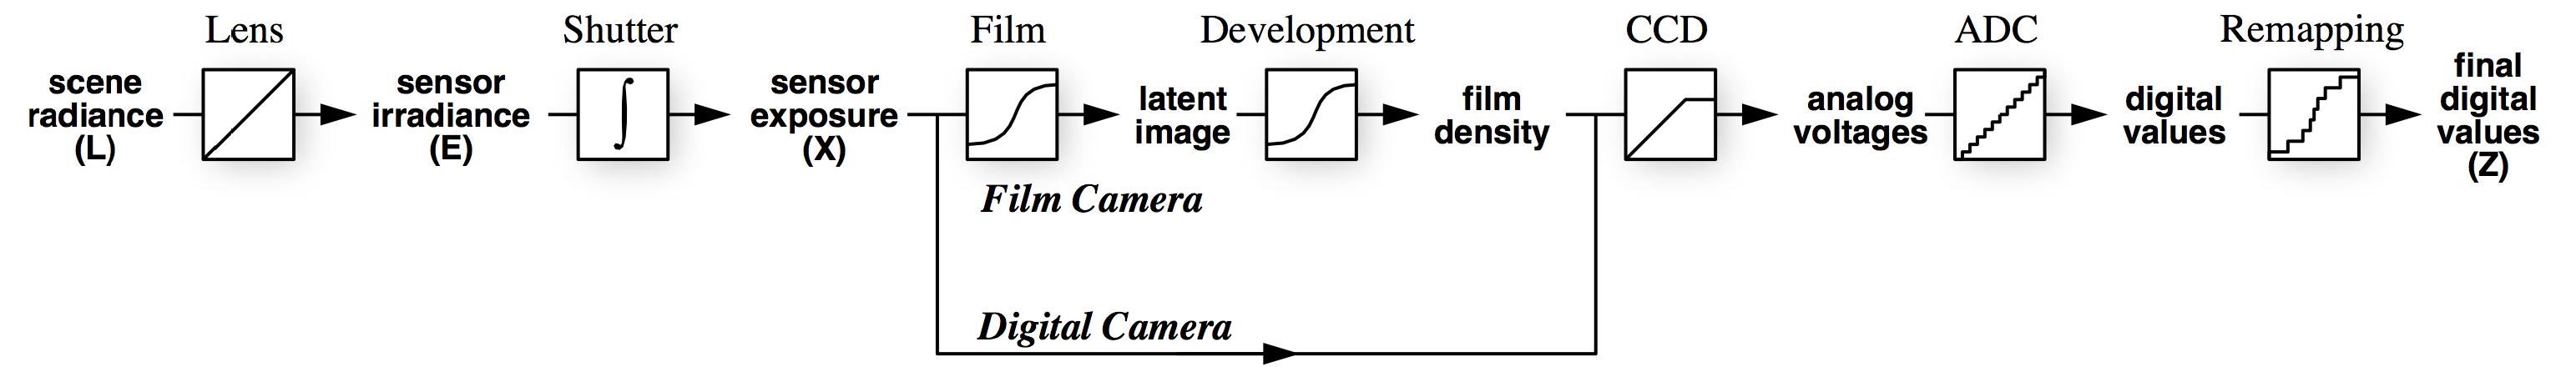
\includegraphics[width=\textwidth]{ImageAquisitionPipeline}
    \caption{\textit{Bildaufnahme Pipeline} --- Veranschaulichung der zu durchlaufenden Prozesse bei der Aufnahme eines Bildes mit einer Kamera  \cite[S.2]{paper}.}
    \label{fig:antwortkurve}
  \end{center}
\end{figure}

Trotz der allgemeinen Formulierung hat das Verfahren von Debevec und Malik jedoch auch einige Schwachstellen. Zum einen werden weder im Daten- noch im Glattheitsterm robuste Bestrafungsfunktionen verwendet. Diese könnten den Ansatz deutlich robuster unter Fehlmessungen machen. Zum anderen werden keine Beschränkungen gefordert, die die typischerweise gewünschte Monotonie der Antwortkuve explizit erzwingen würden. Monotone Kurven können deshalb nur bei einer hinreichend großen Gewichtung der Glattheit erzielt werden. Schließlich ist das Verfahren auch nicht sonderlich robust gegenüber Rauschen, was insbesondere bei sehr kurz belichteten Bildern Probleme bereiten kann. 

\section{Aufgabenstellung}
Ziel der Arbeit ist es zunächst das Verfahren von Debevec und Malik \cite{paper} als Ausgangsverfahren in einer (dafür sinnvollen und portierbaren) Programmiersprache zu implementieren.

Diese Implementierung soll anschließend sukzessive um eine Monotonie-Beschränkung (siehe \autoref{sec:monotonie}), einen räumlichen Glattheitsterm (siehe \autoref{sec:raeumlich}) und robuste Bestrafungsfunktionen (siehe \autoref{sec:robustheit}) erweitert werden.

\begin{figure}[H]
  \begin{center}
      \begin{overpic}[width=0.48\textwidth]{teezer/E_noise_no_robustness}
                \put(-0,0){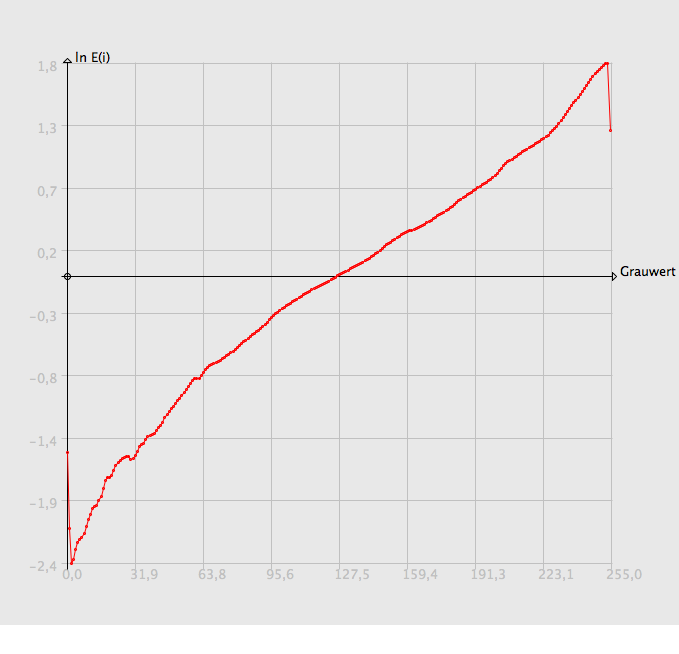
\includegraphics[width=2cm]{teezer/g_noise_no_robustness}}
        \end{overpic}
        \hfill
        \begin{overpic}[width=0.48\textwidth]{teezer/E_noise_robustness_raum}
            \put(-0,0){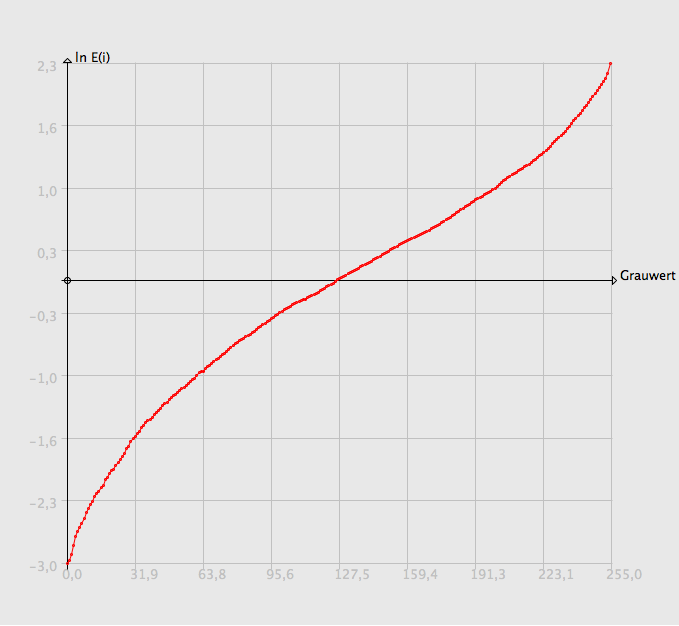
\includegraphics[width=2cm]{teezer/g_noise_robustness_raum}}
        \end{overpic}
    \caption{\textit{Antwortkurven (incl. zugehörigem HDR-Bild)} --- Das HDR-Bild wurde mittels lokalem Reinhard-Tone-Mapper (siehe \autoref{subsec:ToneMapping}) erstellt. \textbf{links}: Ohne robuste Bestrafungsterme. \textbf{rechts}: Mit robusten Bestrafungstermen und räumlicher Glattheitsforderung.}
    \label{fig:teezer}
  \end{center}
\end{figure}


Neben der Modellierung und Implementierung der einzelnen Erweiterungen soll auch eine geeignete visuelle Evaluation der Ergebnisse erfolgen. Hierzu sollen \gls{Tone-Mapping}-Verfahren (siehe \autoref{subsec:ToneMapping}) aus bereits existierender Forschung verwendet werden. 


\section{Gliederung}
Die Arbeit gliedert sich wie folgt:
\begin{description}

\item[\autoref{chap:hdr} -- \nameref{chap:hdr}:] Hier werden die Grundlagen der \gls{HDR}-Bilder vermittelt. Dabei wird auf die physikalischen, historischen und anwendungsorientierten Eigenschaften von \gls{HDR}-Bildern eingegangen.

\item[\autoref{chap:references} -- \nameref{chap:references}:] Anschließend werden verwandte Arbeiten zum Thema \gls{HDR} vorgestellt.

\item[\autoref{chap:algo} -- \nameref{chap:algo}:] Die zu Grunde liegende Vorgehensweise von Debevec und Malik soll in diesem Kapitel beschrieben werden. Außerdem werden die existierenden Schwachstellen des bisherigen Ansatzes dargestellt.

\item[\autoref{chap:maths} -- \nameref{chap:maths}:] Der theoretische Ansatz aus \autoref{chap:algo} wird hier mathematisch umgesetzt und diskutiert. Außerdem werden die Erweiterungen des Algorithmus beschrieben und formal spezifiziert.

\item[\autoref{chap:impl} -- \nameref{chap:impl}:] Dieses Kapitel beschäftigt sich mit der Herangehensweise an die Problemstellung aus Sicht der Entwicklung. Es werden Anforderungen an die Software formuliert, der Prototyp vorgestellt und die Architektur der Implementierung beschrieben. Abschließend wird die Verwendung der Software erläutert.

\item[\autoref{chap:results} -- \nameref{chap:results}:] Anschließend werden die Resultate und Einflüsse der unterschiedlichen Erweiterungen vorgestellt und diskutiert.

\item[\autoref{chap:zusfas} -- \nameref{chap:zusfas}:] Zusammenfassung der Ergebnisse der Arbeit und Darstellung von Anknüpfungspunkten zu weiteren Arbeiten.
\end{description}

%\setchapterpreamble[u]{%
%\dictum[Albert Einstein]{Probleme kann man niemals mit derselben Denkweise lösen, durch die sie entstanden sind.}
%}

\chapter{Grundlagen der HDR-Bilder}
\label{chap:hdr}


In den vergangenen Jahren hat die digitale Fotografie zu einem Umdenken und einer Neuschaffung von Kommunikationskanälen geführt. 
Durch die Verbreitung von Digitalkameras (insbesondere auch solchen, die in Smartphones und Handys eingebaut sind) können Nachrichten in Form von Fotografien in Sekundenschnelle über den ganzen Globus geschickt werden. In Diensten wie \texttt{Twitter}, \texttt{Instagram} oder \texttt{Vine} werden Bilder und Videos in riesigen Mengen verschickt. Nach aktuellen Zahlen werden z.B. in \texttt{Instagram} täglich 55 Millionen Bilder gepostet\footnote{\url{http://instagram.com/press/}}. In diesem Zuge spielt auch die digitale Bildbearbeitung eine immer größer werdende Rolle. 

Digitalbilder werden in der heutigen Zeit hauptsächlich in Form der drei Farbkanäle Rot, Grün und Blau dargestellt (sog. RGB-Farbraum). Häufig kommt noch ein vierter Kanal, der sog. Alpha-Kanal hinzu, der für die Darstellung von Transparenz genutzt wird. 

Jeder Kanäle wird in der Regel mittels eines Bytes repräsentiert. Damit können 16,7 Millionen verschieden Farben dargestellt werden. Trotz dieser großen Zahl sind nur 256 verschiedene Werte für jeden Farbkanal möglich. Diese Anzahl ist häufig unzureichend, um Szenen mit hohen Helligkeitsunterschieden zu repräsentieren \cite[S.~1f]{Reinhard}.


\begin{figure}
  \begin{center}
    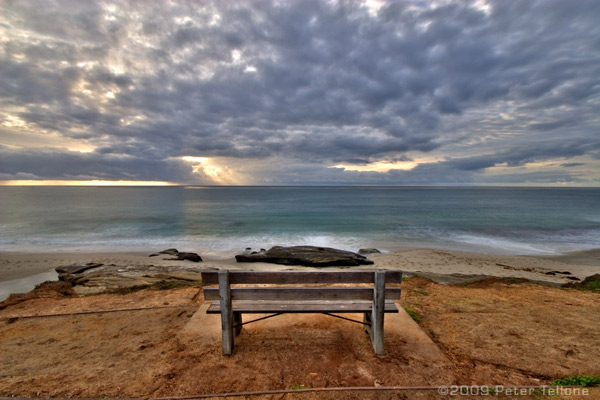
\includegraphics[width=0.6\textwidth]{example}
    \caption{HDR-Bild mit bereits angewandtem \gls{Tone-Mapping}-Verfahren \cite{tellone}}
    \label{fig:teezer}
  \end{center}
\end{figure}

Die Verwendung von \gls{HDR}-Bildern kann diese Problematik beheben. Ziel ist es, mehr Farben und Details in unterschiedlichen Bildbereichen sichtbar zu machen. Um dies zu ermöglichen, erhöht man bei \gls{HDR}-Bildern den \gls{Dynamikumfang} des Bildbereiches. Dazu ist jedoch eine andere Form der Repräsentation des Bildes notwendig (sog. \glspl{Radiance Map}).

%------------------------------------------------------------------------------------------------------------
\section{Prinzip}

Das menschliche Auge kann in einer täglichen Szene einen \gls{Dynamikumfang} im Bereich von 1:10.000 wahrnehmen \cite{Fairchild04theicam}. Dieser Umfang liegt weit über den herkömmlichen Werten eines normalen Kamera-Sensors. In der \autoref{tab:illumination} sind verschiedene Dynamikumfänge (und die damit zusammenhängende Belichtungsstärke) aufgelistet. 
Um mit \gls{HDR}-Bildern einen höheren \gls{Dynamikumfang} darstellen zu können, müssen mehr Informationen als über den herkömmlichen Weg beschaffen werden. Dazu werden entweder mehrere Bilder mit verschiedenen Belichtungszeiten zu einer \gls{Radiance Map} kombiniert oder es werden spezielle Kamera-Sensoren eingesetzt, welche in der Lage sind eine höhere Dichte an Bildinformationen (z.B. große Helligkeitsunterschiede) aufzunehmen \cite{Yang99a640}. 


\begin{table}
  \begin{center}
    \begin{tabular}{ccc}
	\toprule
	Umgebung & Belichtungsstärke ($cd/m^2$)\\ \midrule
	Sternenhimmel & $10^{-3} $\\	
	Mondschein & $10^{-1} $\\	
	Innenraum Beleuchtung & $10^{2} $\\	
	Sonnenlicht & $10^{5} $\\	
	\midrule
	Herkömmliche Monitore & $10^{2} $\\	
	\bottomrule
    \end{tabular}
    \caption{Belichtungsstärken in verschiedenen Umgebungen \cite[S.~6]{Reinhard}}
    \label{tab:illumination}
  \end{center}
\end{table}



Der hier verwendete Begriff \enquote{\gls{Dynamikumfang}} beschreibt das Verhältnis zwischen dem hellsten und dunkelsten Pixel im Bild. Um Ausreißer weniger zu berücksichtigen und die Messung robuster zu machen, werden manchmal auch Quantile verwendet, um Rauschen in der Eingabe weniger zu gewichten. Bei Bildschirmen wird hingegen unter dem \gls{Dynamikumfang} das Verhältnis zwischen der maximalen und minimalen Leuchtkraft verstanden \cite[S.~4]{Reinhard}.

\begin{figure}[H]
  \begin{center}
    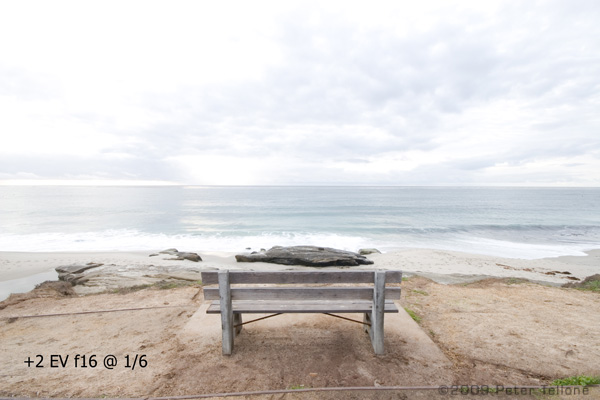
\includegraphics[width=2cm]{img/1_6}
    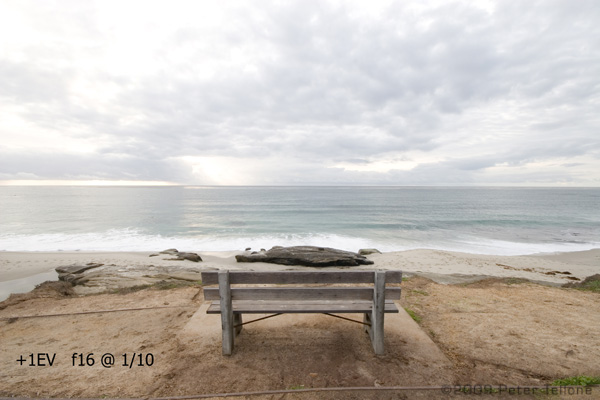
\includegraphics[width=2cm]{img/1_10}
    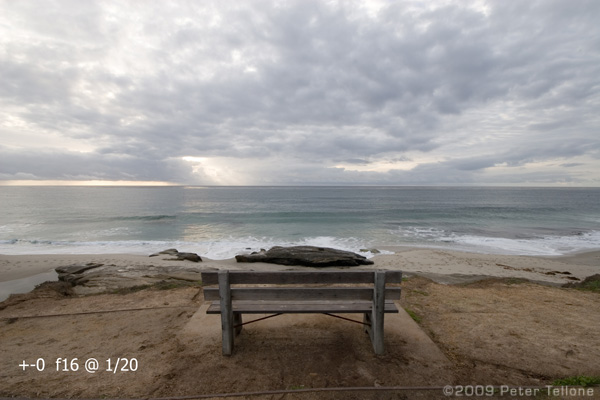
\includegraphics[width=2cm]{img/1_20}
    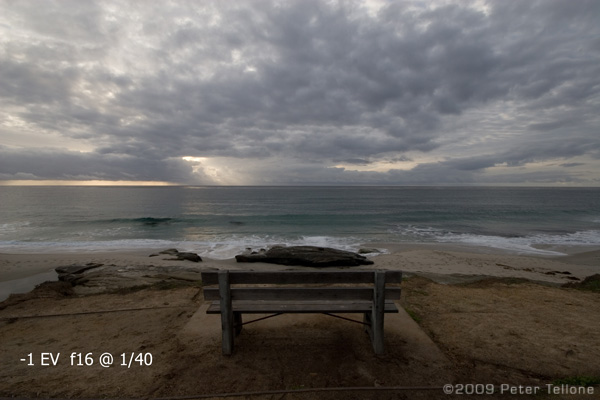
\includegraphics[width=2cm]{img/1_40}
    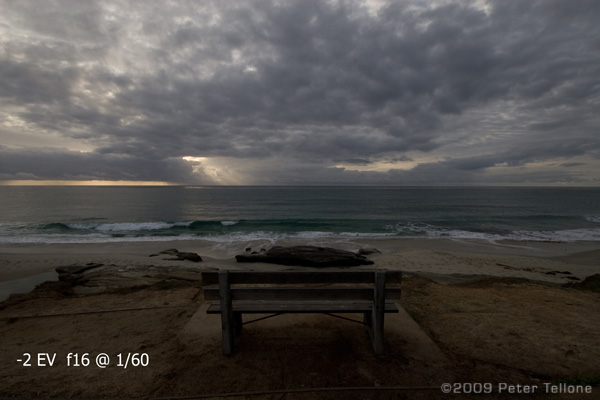
\includegraphics[width=2cm]{img/1_60}
    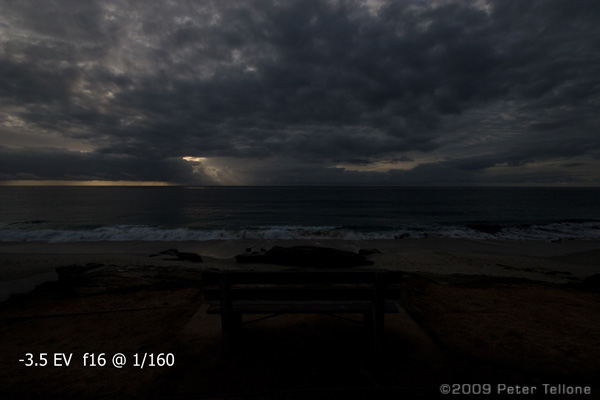
\includegraphics[width=2cm]{img/1_160}
    \caption{\textit{Verwendete Belichtungsserie} --- Sechs Einzelaufnahmen mit den Belichtungszeiten $\frac{1}{6}, \frac{1}{10}, \frac{1}{20}, \frac{1}{40}, \frac{1}{60}\mbox{ und }\frac{1}{160}$ (v.l.n.r) \cite{tellone}}
    \label{fig:teezer}
  \end{center}
\end{figure}




%------------------------------------------------------------------------------------------------------------

\section{Anwendungsgebiet und Geschichte}

Die Möglichkeiten des Einsatzes von \gls{HDR}-Bildern sind vielfältig. Die nachfolgende Liste umfasst einige der Gebiete, in denen diese Technologie eingesetzt wird oder werden kann \cite[S.~87f]{Reinhard}.

\begin{description}

\item[Digitale Fotografie:] Die verschiedenen Kamera-Hersteller gehen bereits immer mehr in Richtung der sog.  \enquote{aufnahmeabhängigen Daten}. In diesen sind bereits häufig mehr Bildinformationen enthalten. Dabei handelt es sich bei verschiedenen Herstellern in der Regel jedoch auch um verschiedene \acrfull{RAW}, die meist nicht kompatibel sind. 

\item[Satellitenbilder:] Satellitenbilder beinhalten in aller Regel sehr viel mehr Informationen als nur den sichtbaren Bereich des Lichtspektrums. \gls{HDR}-Bilder sind hier von Bedeutung, da sie multispektrale Aufnahmen ermöglichen.

\item[Visualisierungen und Rendering:] Eine der ersten Anwendungen waren vermutlich die ersten Render-Engines von Visualisierungen (Computer-Spiele, medizinische Visualisierungen und Simulationen, etc.). Bei manchen Anwendungen ist es insbesondere für Reflektionen wichtig, auch nicht sichtbare Frequenzen bei Berechnungen mit einzubeziehen, da diese durch Interferenzen wieder sichtbar werden können und somit der Detailgrad steigt.

\item[Bildbearbeitungssoftware:] Die großen Bildbearbeitungsanwendungen bieten mittlerweile in der Regel auch die Bearbeitung und Generierung von \gls{HDR}-Bildern an. Als Beispiele sind hier Adobe Photoshop\footnote{\url{http://adobe.com/photoshop}}, Photogenics\footnote{\url{http://www.cinepaint.org}} und Photomatix\footnote{\url{http://www.hdrsoft.com/download.html}} genannt.

\item[Medizin:] In der Endoskopie besteht ein großer Bedarf an immer höher auflösenden \gls{CMOS} Bildsensoren. Diese können immer bessere Aufnahmen aus dem Inneren des Körpers liefern und ermöglichen der Medizin große Fortschritte. Solche Sensoren können bereits in der Größe eines Streichholzkopfes einen Dynamikumfang von 179 dB erreichen \cite{Klingler_Richter_Strobel_2006}.

\item[Virtual Reality:] In Anwendungen, bei denen sich der Benutzer in einem virtuellen Raum bewegt, wird die Wahrnehmung zunehmend wichtig. Auch hier spielen deshalb hohe Dynamikumfänge eine besondere Rolle. In diesem Bereich ist es besonders wichtig, gute Kompressions-Algorithmen für \gls{HDR}-Bilder zu entwickeln, um eine schnelle Übertragung zu gewährleisten. Auch beim Platzieren von synthetischen Objekten in realen Szenen können \gls{HDR}-Bilder eingesetzt werden, um dem Betrachter eine noch \enquote{realere} Szene zu suggestieren \cite{Debevec:2008:RSO:1401132.1401175}.
\end{description}

%------------------------------------------------------------------------------------------------------------
\section{Bilderzeugung}
Für die Erstellung von \gls{HDR}-Bildern gibt es unterschiedliche Möglichkeiten. Dabei muss man jedoch zwischen echten \gls{HDR}-Bildern und Pseudo-\gls{HDR}-Bildern unterscheiden. Im Nachfolgenden werden die verschiedenen Verfahren kurz beschrieben. Der Fokus liegt jedoch auf dem letzten Verfahren, der \nameref{sub:belichtungsreihe}, da dieses Verfahren auch im Ausgangsverfahren von Debevec und Malik verwendet wird.


\subsection{Pseudo-\gls{HDR}-Bilder}
Bei Pseudo-\gls{HDR}-Bildern handelt es sich um eine einfache Fusion von Bildreihen. Deswegen werden diese Verfahren auch Exposure Blending oder Exposure Fusion genannt. Bei dieser Technologie geht es darum, mehr Details aus einer Belichtungsreihe von \acrshort{LDR}-Bildern (\acrlong{LDR} Bilder) zu generieren, ohne dabei ein \gls{HDR}-Bild zu erzeugen. Die Bilder der Belichtungsreihe werden dazu einfach fusioniert \cite{Jing_Hong_Zheng_Rahardja_2012}.

\subsection{HDR-Kameras} 
Diese speziellen Kameras verfügen über Bildsensoren, die von sich aus einen höheren Dynamikumfang aufnehmen können und dadurch bereits die notwendigen Informationen in einer Aufnahme generieren können. Diese Spezial-Kameras sind jedoch noch sehr teuer und wenig verbreitet \cite[S. 95ff]{Bloch2012}. Digitale Spiegelreflex-Kameras bieten mittlerweile häufig ebenfalls einen \gls{HDR}-Modus an.

\subsection{HDR-Bildgenerierung aus einer Belichtungsreihe}
\label{sub:belichtungsreihe}
Um ein \gls{HDR}-Bild aus einer Belichtungsreihe zu erzeugen, braucht man zunächst eine Grundlage für das Bild. In diesem Verfahren werden mehrere Bilder der selben Szene mit unterschiedlichen Belichtungszeiten fusioniert. Ziel der dabei verwendeten Algorithmen ist es, aus diesen Bildern ein \gls{HDR}-Bild zu erzeugen.

Um die Bilder später weiter zu verarbeiten, müssen diese jedoch zunächst registriert werden. Dies ist aufgrund der verschiedenen Belichtungswerte der Aufnahmen häufig nicht oder nur schlecht über Kantendetektions-Verfahren möglich, da diese Merkmale unter den unterschiedlichen Belichtungen sehr stark variieren können.

Ein besserer Ansatz um Bilder zu registrieren ist der \gls{MTB} Ansatz (siehe \autoref{subsec:MTB}). Auf eine Implementierung dieses Verfahrens wurde verzichtet, da es nicht relevant für die Zielsetzung ist.

%------------------------------------------------------------------------------------------------------------
\section{Bildformate und -speicherung}

Für die Abspeicherung der \gls{HDR}-Bilder werden in \autoref{tab:formats} die drei gängigsten Formate mit den dazu gängigen Kodierungen verglichen \cite[S.~89]{Reinhard}. Die Speicherung der erzeugten Daten war kein zentraler Bestandteil der vorliegenden Arbeit und wurde deshalb bei der Realisierung nicht berücksichtigt. Dennoch sollen hier die bekanntesten Kodierungen zur Abspeicherung vorgestellt werden.


\begin{table}[H]
  \begin{center}
    \small
    \begin{tabularx}{\textwidth}{l|XXXX}
	\toprule
	Format & Kodierung & Kompression & Metadaten & Lizenz \\
	\midrule
	HDR & RGBE & Laufl"angen-\newline kodierung & Kallibrierung, \newline Farbraum & Open source\newline software (\textit{Radiance})\\
	& XYZE & Laufl"angen-\newline kodierung & + benutzerdef. Daten & \\
	\midrule
	TIFF & IEEE RGB & keine & Kallibrierung, \newline Farbraum & Public domain \newline library (\textit{libtiff})\\
	& LogLuv24 & keine &+ Registrierung \newline+ benutzerdef. Daten& \\
	& LogLuv32 & Lauflängen-\newline kodierung & & \\
	\midrule
	EXR & Half RGB & Wavelet, ZIP & Kallibrierung, \newline Farbraum \newline+ Fensterfunktion \newline+ benutzerdef. Daten & Open source library (\textit{OpenEXR})\\
	\bottomrule
    \end{tabularx}
    \normalsize
    \caption{\textit{HDR-Bildformate} --- Die verbreitetsten Formate und ihre Eigenschaften in der Übersicht \cite[S.89]{Reinhard}.}
    \label{tab:formats}
  \end{center}
\end{table}


\subsection{RGBE -- Das .hdr Format}

Dieses Format wurde ursprünglich unter den Dateiendungen \texttt{.hdr} und \texttt{.pic} eingeführt. Abgesehen von den Metadaten (wie z.B. Bildgröße, Ausrichtung, notwendige Angaben zur verwendeten Kodierung, etc.) werden die Bildpunkte mit 32-Bit dargestellt. Diese umfassen die Kanäle für Rot, Grün und Blau sowie einen Exponenten, was zu einer Vergrößerung des Dynamikbereiches führt \cite[S. 92]{Reinhard}.

\subsection{TIFF -- Gleitkomma Kodierung}
\label{sub:tiff}
Das Format \texttt{.tiff} enthält eine 32-Bit Kodierung pro Komponente (also 96-Bit für einen Bildpunkt). Dabei werden die Bildpunkte mittels Fließkommazahlen dargestellt \cite{adobe:tiff}. Dieser Standard unterstützt bereits eine sehr hohe Genauigkeit. Dazu benötigt dieses Dateiformat im Vergleich zu anderen jedoch auch am meisten Speicherplatz. Allerdings lässt sich damit auch eine nahezu verlustfreie Abspeicherung von \gls{HDR}-Bildern erreichen. Im Standard von 1992 wurde auf jede Form der Komprimierung verzichtet \cite[S. 93]{Reinhard}. Dieser kann jedoch um verschiedene Kompressionsverfahren erweitert werden. \texttt{LogLuv} ist beispielsweise ein solches, bei dem die Werte logarithmisch skaliert und quantisiert werden \cite{logluv}. 


\subsection{EXR -- EXtended Range Format}

Dieses Format wurde 2002 veröffentlicht\footnote{\url{www.openexr.com}} und basiert ebenfalls auf der Speicherung von Fließkommazahlen. Es existiert eine Variante bei der nur 16 Bit (Hälfte der normalen Anzahl) für das Speichern der Fließkommazahlen verwendet wird: ein Bit für das Vorzeichen, fünf für den Exponenten und zehn für die Mantisse. Für diese Komprimierung sind Quantisierungsschritte von unter 0.1\% vorgesehen und damit für das menschliche Auge nicht erkennbar. Dadurch ist diese Kompression quasi verlustfrei durchführbar \cite[S. 97f]{Reinhard}.

%------------------------------------------------------------------------------------------------------------
\section{Bilddarstellung}
\label{subsec:ToneMapping}
 Für die Darstellung der \glspl{Radiance Map} gibt es vereinzelt spezielle Hardware, die in der Lage ist den erweiterten Dynamikumfang darzustellen. Sehr viel häufiger kommen jedoch sog. \gls{Tone-Mapping} (dt.: Dynamikkompressions) Verfahren zum Einsatz. Diese stellen ein HDR-Bild durch eine andere Skalierung des Bildbereichs als herkömmliche Bilddateien dar. 
 
 Der Kerngedanke beim \gls{Tone-Mapping} besteht darin, einen geeigneten Weg für die Zuordnung von Bildpunkten aus dem \gls{HDR}-Bild in das \gls{LDR} Bild zu finden \cite[S. 145]{Bloch2012}. Diese Zuordnungsfunktionen nennen sich \gls{Tone-Mapping}-Operatoren und können generell in zwei Kategorien unterschieden werden. Die globalen Operatoren (siehe \autoref{sub:tone:global}) bearbeiten alle Bildpunkte gleich, während die lokalen Operatoren (siehe \autoref{sub:tone:local}) Informationen aus der Umgebung in die Berechnung an jedem Bildpunkt mit einbeziehen.
 

 \subsection{Globale \gls{Tone-Mapping}-Operatoren}
\label{sub:tone:global}
Bei globalen \gls{Tone-Mapping}-Operatoren wird die gesamte Farbkurve (engl. tone curves) modifiziert. Die Veränderungen können auf den verschiedenen Farbkanälen unterschiedlich sein. Auch die Berechnung der modifizierten Kurve kann sich aufgrund des Bildes ändern \cite[S. 146]{Bloch2012}. 

Es bestehen viele verschiedene Ansätze für globale \gls{Tone-Mapping}-Operatoren, die unterschiedliche Vor- und Nachteile aufweisen.
In dieser Arbeit wurde lediglich der \gls{Tone-Mapping}-Operator von Reinhard et al. \cite{ReinhardToneMapper} implementiert und verwendet. Dabei handelt es sich um die vereinfachte Form des komplexeren lokalen Operators, der im gleichen Artikel veröffentlicht wurde.
Hierzu wird zunächst der durchschnittliche Wert des Logarithmus aus der Helligkeit des Bildes $L_w(x,y)$ bestimmt. Dieser wird als charakteristischer Wert der Szene $\tilde{L}_w$ beschrieben. Anschließend werden die skalierten Helligkeiten des Bildes errechnet (siehe \autoref{eq:skaled:greyvalues}). $\alpha$ bestimmt die Lage des mittleren Grauwertes und hat in der Regel den Wert $0.18$. Daraus lässt sich dann der globale Operator in \autoref{eq:tonemapping:global} erstellen.
\begin{align}
\label{eq:skaled:greyvalues}
L(x,y) = \frac{\alpha}{\tilde{L}_w} L_w(x,y)\\
\label{eq:tonemapping:global}
L_d(x, y) =\frac{L(x,y)}{1+ L(x,y)}
\end{align}


\subsection{Lokale \gls{Tone-Mapping}-Operatoren}
\label{sub:tone:local}

Lokale \gls{Tone-Mapping}-Operatoren können bei der Zuordnung eines Wertes aus einem \gls{HDR}- in ein \gls{LDR}-Bild auch die lokale Umgebung eines jeden Bildpunktes berücksichtigen. Damit erreichen sie in sehr dynamischen Bildern bessere Ergebnisse und können mehr Details in Bildern hervorheben. Auch hier gibt es eine Vielzahl verschiedener Operatoren, die alle ihre Vor- und Nachteile haben. Da der Operator von Reinhard et. al \cite{ReinhardToneMapper} in verschiedenen Veröffentlichungen \cite{tone_mapper_1,tone_mapper_2} gut abgeschnitten hat, wird dieser verwendet.

Bei diesem handelt es sich um einen lokalen \gls{Tone-Mapping}-Operator, der dodging-and-burning (dt. abwedeln) zur Berechnung verwendet. Dieses Verfahren ist eine Technik, die aus der analogen Fotografie stammt. Dabei wird die Belichtungszeit in einzelnen Bereichen des Bildes verändert, um diese bei der Entwicklung des Filmmaterials differenziert zu behandeln. Die Wahl der einzelnen Bereiche wird im technischen Ansatz durch die Berechnung des lokalen Kontrastes im Bild umgesetzt, welche die Reichweite des Operators beeinflussen.

Auf eine weitere Beschreibung des Verfahrens wird hier aus Gründen der Komplexität verzichtet.


%------------------------------------------------------------------------------------------------------------
\section{Software zur Erstellung von HDR-Bildern}
\label{sec:software}
Herkömmlich Programme zur Bildbearbeitung (z.B. \texttt{Photoshop}\footnote{\url{http://adobe.com/photoshop}} oder \texttt{GIMP}\footnote{\url{http://www.gimp.org} mit Plugin \texttt{Exposure Blend} (\url{http://tir.astro.utoledo.edu/jdsmith/code/exposure_blend.php})}) unterstützen die Erzeugung von \gls{HDR}-Bildern aus einer Belichtungsserie recht gut. Es gibt in der Regel mehrere \gls{Tone-Mapping}-Operatoren, deren Parameter anschaulich verändert werden können. Diese trumpfen mit hohem Funktionsumfang, vielfältigen Einstellungsvarianten und der Möglichkeit der weiteren Bearbeitung auf.


\begin{figure}[h]
  \begin{center}
    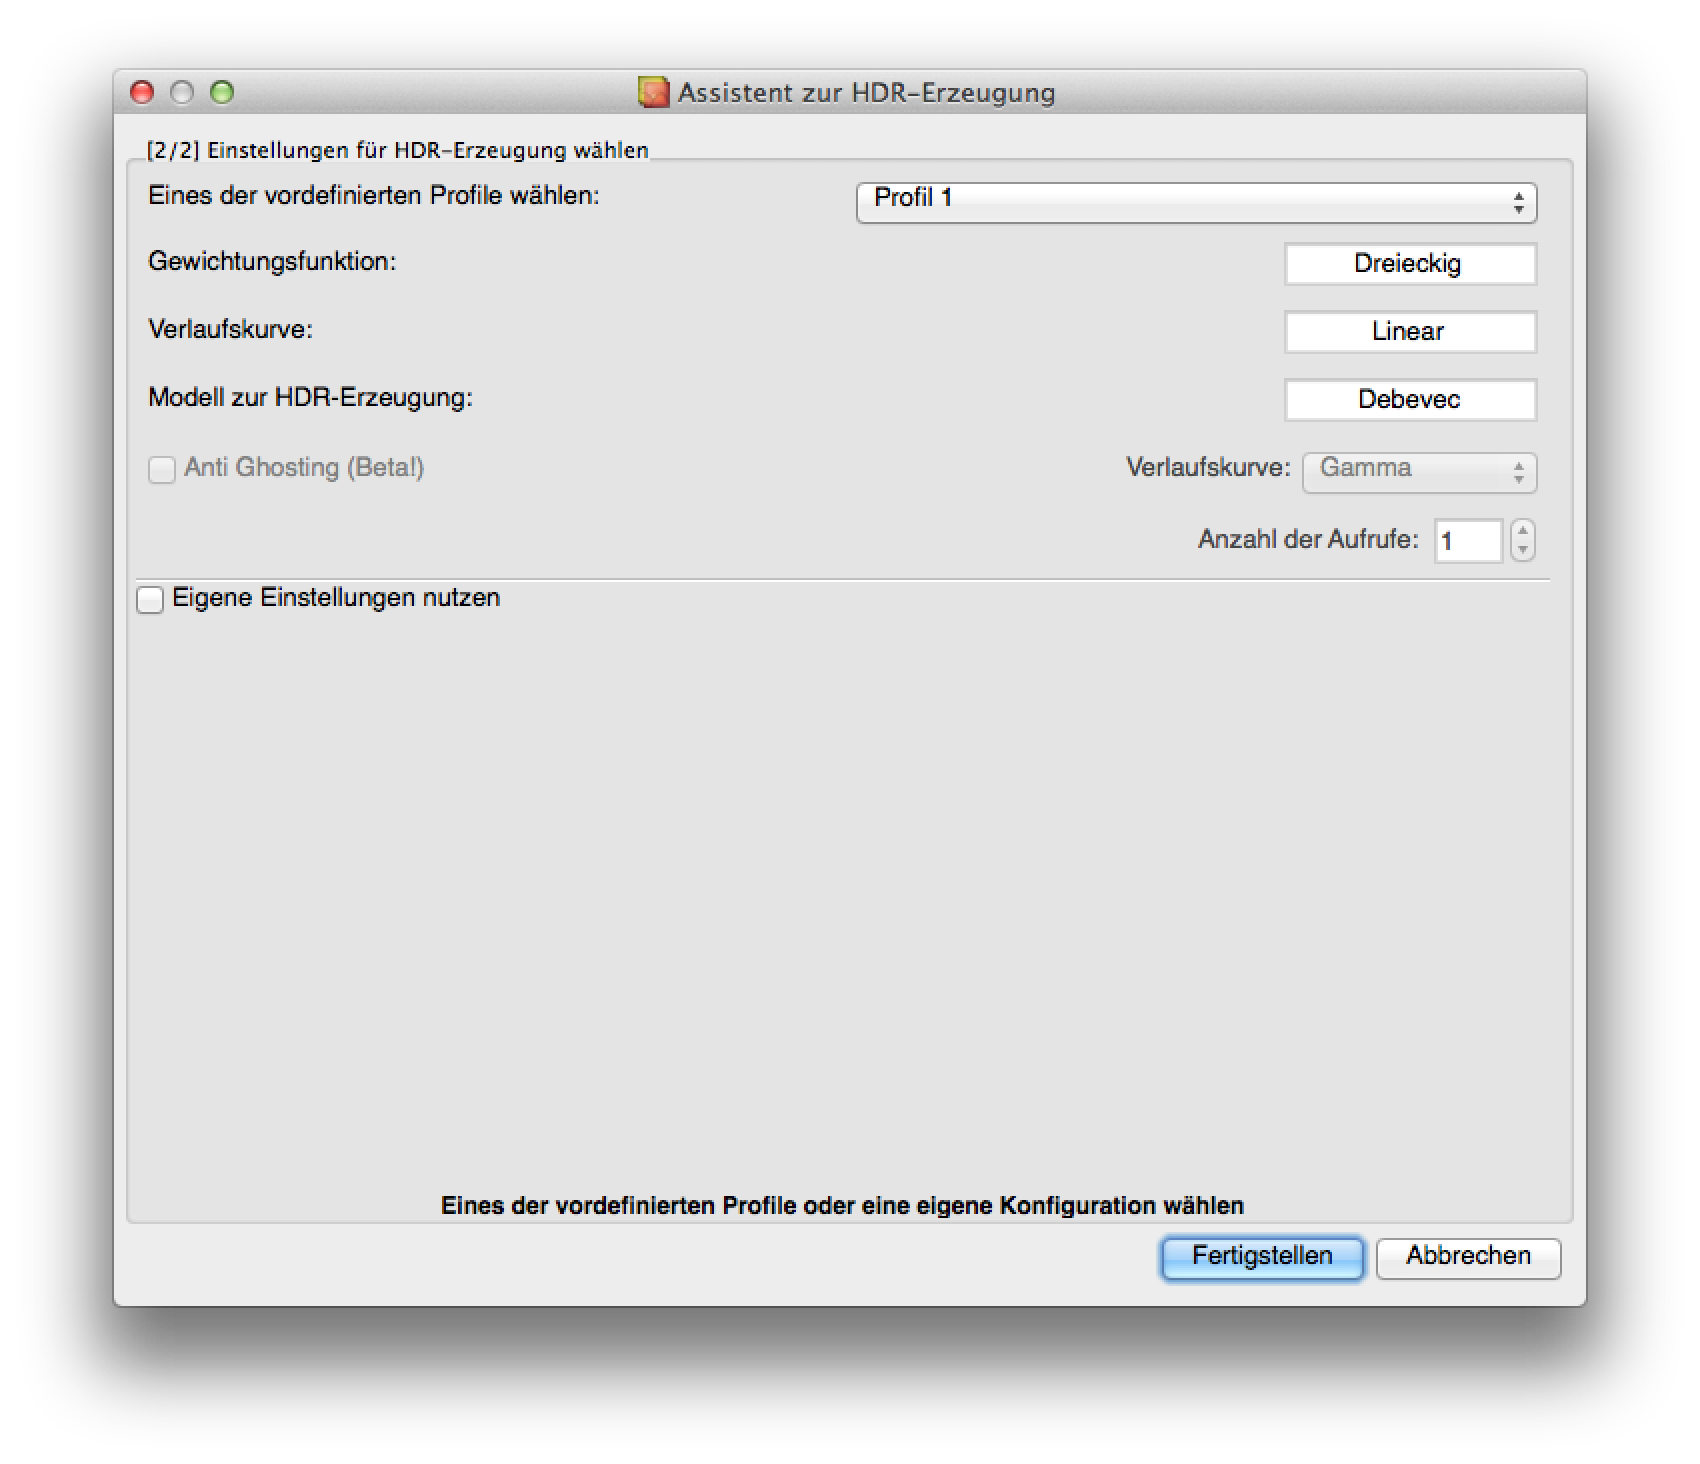
\includegraphics[width=0.8\textwidth]{Luminance}
    \caption{\textit{Erstell-Assistent von \texttt{Luminance HDR}} --- Auch hier wird intern der Algorithmus von Debevec und Malik verwendet.}
    \label{fig:luminance}
  \end{center}
\end{figure}

Darüber hinaus gibt es verschiedene Programme, die speziell auf die Erzeugung von \gls{HDR}-Bildern spezialisiert sind (z.B. \texttt{Photomatix}\footnote{\url{http://www.hdrsoft.com/de/}, kostenpflichtig} oder \texttt{Luminance HDR}\footnote{\url{http://qtpfsgui.sourceforge.net}, Freeware}). Der Funktionsumfang dieser Programme ist verhältnismäßig klein, führt jedoch auch Laien schnell zum Ziel, da (wie z.B. bei \texttt{Luminance HDR}, siehe \autoref{fig:luminance}) interaktive Assistenten den Benutzer bei der Erstellung anleiten. 


\begin{figure}
  \begin{center}
    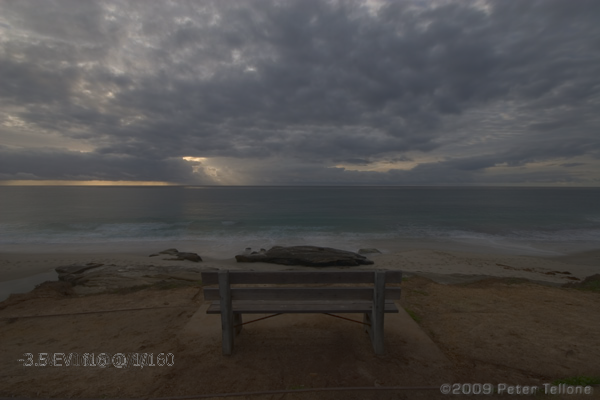
\includegraphics[width=0.8\textwidth]{BenchGeneratedLuminance}
    \caption{\textit{Ergebnis eines HDR-Bildes} --- Hier erstellt mit \texttt{Luminance HDR} und dem \gls{Tone-Mapping}-Operator \texttt{Reinhard'05} \cite{Reinhard05}, Bildserie siehe \cite{tellone}.}
    \label{fig:luminance}
  \end{center}
\end{figure}

Als weitere Beispiele für \gls{HDR}-Software seien hier außerdem \texttt{Dynamic-Photo HDR}\footnote{\url{http://www.mediachance.com/hdri/index.html}, kostenpflichtig} und \texttt{HDR Darkroom}\footnote{\url{http://www.everimaging.com}, kostenpflichtig} genannt. Diese haben sehr viele \gls{Tone-Mapping}-Operatoren implementiert und können sowohl realistische als auch sehr verfremdete \gls{HDR}-Bilder generieren. 

Ein wirklich einfaches Programm ist \texttt{Picturenaut}\footnote{\url{http://www.hdrlabs.com/picturenaut/}, Freeware}. Die Anzahl und der Funktionsumfang der implementierten \gls{Tone-Mapping}-Operatoren ist limitiert, jedoch liefert das Programm recht rasch realitätsgetreue Bilder.



%\setchapterpreamble[u]{%
%\dictum[Albert Einstein]{Probleme kann man niemals mit derselben Denkweise lösen, durch die sie entstanden sind.}
%}
\chapter{Verwandte Arbeiten und Implementierungen}
\label{chap:references}

In diesem Kapitel soll kurz auf verwandte Arbeiten und Implementierungen eingegangen werden. Der Fokus liegt bei der nachfolgenden Recherche auf dem Ansatz aus einer Belichtungsserie von \gls{LDR}-Bildern ein \gls{HDR}-Bild zu generieren.

\section{Bekannte Implementierungen des Ansatzes von Debevec und Malik}
\label{sec:implementations}
Das Standard-Verfahren als solches wurde bereits in verschiedenen Programmen implementiert. Am ursprünglichen Artikel von Debevec und Malik ist bereits eine \texttt{MATLAB}-Version des Algorithmus angefügt. 
Darauf basierend hat z.B. Mathias Eitz eine Implementierung\footnote{\url{http://cybertron.cg.tu-berlin.de/eitz/hdr/index.html}} des kompletten Prozesses in \texttt{MATLAB} geschrieben. Dieser arbeitet ohne Erweiterungen und implementiert direkt den beschriebenen Ansatz. Die \nameref{algo:schwachstellen:selektion} (siehe \autoref{algo:schwachstellen:selektion}) geschieht in dieser Implementierung in einer Art Rasterung der Bilder und berücksichtigt keine der Forderungen von Debevec und Malik (siehe \autoref{algo:schwachstellen:selektion}). 

Auch in der bereits genannten Software zur Erstellung von \gls{HDR}-Bildern (siehe \autoref{sec:software}) wird z.T. der Ansatz von Debevec und Malik verwendet.


\section{Verwandte Arbeiten}

In den letzten Jahren haben die veröffentlichten Arbeiten zur Generierung, Darstellung und Verarbeitung von \gls{HDR}-Bildern stetig zugenommen. Mit der nachfolgenden Auswahl von verwandten Arbeiten soll ein Überblick über den Themenbereich geschaffen werden.

Jinno and Okkuda \cite{Jinno} beschreiben in ihrer Alternative für die Fusion von Belichtungsserien (basierend auf herkömmlichen Algorithmen) auch die Problematik von sich bewegenden Objekten. Daraus entstehen bei der Fusion häufig ghosting artifacts (dt. Geist-Artefakte) oder motion blur (dt. Bewegungsunschärfe). In dieser Veröffentlichung werden die bewegten Objekte erkannt und bei der Berechnung des \gls{HDR}-Bildes wieder entfernt. Das Verfahren sagt dabei Überdeckung, Sättigung und Verschiebungen in den Ausgangsbildern voraus und konstruiert die \gls{HDR}-Bilder unter Berücksichtigung dieser Daten. Damit können insbesondere in Serien mit hoher Bewegung bessere Ergebnisse erzielt werden.

Nayar et al. \cite{Nayar00highdynamic} stellen in ihrem Verfahren einen anderen Ansatz der Generierung von \gls{HDR}-Bildern vor. Dabei wird bereits bei der Aufnahme eines Bildes eine Rasterung durch ein optisches Gitter mit unterschiedlichen Transparenzen erzielt. Das so aufgenommene Bild wird als spatially varying exposure (dt. ortsabhängig belichtetes) Bild bezeichnet. Da die Struktur des Gitters und dessen Transparenzen bekannt sind, kann aus dem aufgenommenen Bild nun ein \gls{HDR}-Bild mit höherem Dynamikumfang berechnet werden. Die unterschiedlichen Transparenzen des Gitters sorgen dafür, dass sowohl hohe als auch niedrige Belichtungen wahrgenommen werden können. 

Liu et al. \cite{Xinqiao} beschreiben in ihrem Artikel ein heuristisches Verfahren zur Schätzung der Bewegung in einer Bildserie. Dieses Verfahren basiert auf einem in selbigem Artikel veröffentlichten rekursiven Verfahren bei dem große Belichtungsserien (ihr Beispiel umfasst 65 Aufnahmen) Stück für Stück zu einem \gls{HDR}-Bild zusammengesetzt werden. Ihr Ansatz verspricht besonders bei Bildern mit sehr schnellen Änderungen (wie z.B. einem sich drehenden Propeller) gute Ergebnisse. Die Aufnahmen selbst werden dabei durch herkömmliche \gls{CMOS}-Bildsensoren aufgenommen. Mögliche Messfehler werden im Algorithmus ausgiebig behandelt um Rauschen zu reduzieren.

Im Artikel von Zimmer et al. \cite{zimmer} wird ebenfalls ein Verfahren zur Reduktion von Bewegungsunschärfe bei der Erzeugung von \gls{HDR}-Bildern beschrieben. Hierbei kommt die Berechnung des optischen Flusses bei der Registrierung der Bilder zum Einsatz. Darüber hinaus wird in diesem Verfahren ein hochauflösendes \gls{HDR}-Bild erzeugt, da aus den verschiedenen Bildern der Belichtungsserie durch die Registrierung auch Zwischenpixel-Bereiche mit Informationen gefüllt werden können. Dadurch kann die Auflösung erhöht werden. Mithilfe dieses Verfahrens ist es möglich auch verwackelte Bilder, die Bewegung enthalten, zu registrieren und dadurch ein \gls{HDR}-Bild zu erzeugen.

Auch die \gls{Tone-Mapping}-Operatoren werden ständig untersucht und verbessert. So vergleichen Kuang et al. \cite{tone_mapper_2} in ihrer Studie über \gls{HDR}-Bildgenerierungs-Algorithmen vier lokale und zwei globale Operatoren miteinander. Während der Studie werden verschiedene Bildszenen mit den sechs Operatoren von Probanden in drei unterschiedlichen Experimenten bewertet. Dazu werden die Bilder paarweise auf einem \gls{LDR}-Bildschirm gezeigt. Das Experiment stellte fest, dass keiner der untersuchten Operatoren durchweg in allen Szenen besser als alle anderen Probanden abschneidet. Dies führt zur Schlussfolgerung, dass eine große Korrelation zwischen Szene und \gls{Tone-Mapping}-Verfahren besteht. 

In einer Arbeit von Yoshida et al. \cite{tone_mapper_1} werden sieben \gls{Tone-Mapping}-Operatoren im Direktvergleich der realen Szene und dem korrespondierendem \gls{LDR}-Bild von Testpersonen bewertet. Berücksichtigt wurden dabei sowohl globale als auch lokale Operatoren. Eine der Haupterkenntnisse dieser Studie ist, dass lokale Operatoren die Bilddetails besser beibehalten, wobei globale Operatoren den Kontrast besser darstellen können.


%Die Angabe des schlauen Spruchs auf diesem Wege funtioniert nur,
%wenn keine Änderung des Kapitels mittels den in preambel/chapterheads.tex
%vorgeschlagenen Möglichkeiten durchgeführt wurde.
%\setchapterpreamble[u]{%
%\dictum[Albert Einstein]{Probleme kann man niemals mit derselben Denkweise lösen, durch die sie entstanden sind.}
%}
\chapter{Algorithmus von Debevec und Malik}
\label{chap:algo}
Diese Arbeit behandelt im Kern den Ansatz von Debevec und Malik \cite{paper}. Obwohl der Artikel bereits relativ alt ist (Verfassung 1997), wird das Verfahren noch immer in vielen Anwendungen benutzt (siehe \autoref{sec:implementations}). Dessen Kerngedanke ist es \gls{HDR}-Bilder aus Bildserien zu generieren, welche mit einer herkömmlichen Kamera-Ausrüstung aufgenommen wurden.

\section{Ansatz}
Der Algorithmus schätzt während der Generierung des \gls{HDR}-Bildes gleichzeitig auch die sog. Antwortkurve der Kamera. Diese Antwortkurve ist die kameraspezifische Abbildung, welche aus den Beleuchtungswerten der aufzunehmenden Szene Grau- bzw. Farbwerte erzeugt (siehe \autoref{fig:antwortkurve}). 

Um aus der Belichtungsserie ein \gls{HDR}-Bild erzeugen zu können, müssen die Beleuchtungswerte der Kamera-Sensorik (hier $\b E$) identifiziert werden. Normalerweise geschieht dies indem die Umkehrfunktion der Kamera-Antwortkurve vorab berechnet wird. Dazu muss die Kamera durch Test-Bilder vermessen und das System radiometrisch kalibriert werden. Beim Ansatz von Debevec und Malik wird diese Kamera-Antwortfunktion hingegen während der Generierung des \gls{HDR}-Bildes aus der Belichtungsserie errechnet. Dadurch ist es möglich Belichtungsserien (auch ohne Kenntnisse über die Apparatur) zu \gls{HDR}-Bildern zu fusionieren.


\subsection{Verwendete Symbole}
In den nachfolgenden Beschreibungen werden analog zu \cite{paper} folgende Symbole verwendet:
\begin{align*}
P: &  \mbox{ Anzahl der Bilder der Bildserie (Anzahl der verschiedenen Belichtungszeiten)}\\
N: & \mbox{ Anzahl der Bildpunkte in jedem Bild ($n \times m$ Bild $\Rightarrow N = n \cdot m$)}\\
Z_{i,j} : &\mbox{ Grauwert $i \in [0, N-1]$ des Bildes $j \in [0, P-1]$}\\
Z_{min} : & \mbox{ Minimaler Grauwert $Z_{min} = \min \{Z_{ij}\} \; \forall i,j$ (wird zur Vereinfachung mit $0$ belegt)}\\
Z_{max} : & \mbox{ Maximaler Grauwert $Z_{max} = \max \{Z_{ij}\} \; \forall i,j$ (wird zur Vereinfachung mit $255$ belegt)}\\
E_i : & \mbox{ Beleuchtungsstärke im Pixel $i \in [0, N-1]$ }\\
F_i : & \mbox{ Abkürzende Notation für $\ln E_i$}\\
\Delta t_j : & \mbox{ Belichtungsdauer des Bildes $j \in [0, P-1]$}\\
f(X) : & \mbox{ Nichtlineare Funktion, Belichtung $X$, Grauwertbild $Z$: $f(X) = Z$}\\
\b g(z) : & \mbox{ Kameraantwortkurve als diskreter Vektor (abuse of notation)}\\
\b{g}'(z) : & \mbox{ Diskrete Approximation der ersten Ableitung von }\b g\\
		& \quad \b g'(z) = \b g(z) - \b g(z-1)\\
\b{g}''(z)  : & \mbox{ Diskrete Approximation der zweiten Ableitung von }\b g\\
		& \quad \b g''(z) = \b g(z-1)-2\b g(z)+\b g(z+1)
\end{align*}

\subsection{Herleitung}
Da aus physikalischer Sicht angenommen werden kann, dass $f$ monoton steigend und stetig ist, sei auch $f^{-1}$ definiert. Damit kann die Belichtung $X$ mit $f^{-1}(Z) = X$ berechnet werden. Die Belichtung hängt linear von der Beleuchtungsstärke $E$ und der Belichtungsdauer $\Delta t$ mit $X = E \cdot \Delta t$ ab. Damit ergeben sich die nachfolgenden Zusammenhänge:

\begin{align*}
Z_{ij} &= f(X_{ij})\\
Z_{ij} &=f(E_i \cdot \Delta t_j)&&\text{(siehe oben)}\\
f^{-1}(Z_{ij}) &= E_i \cdot \Delta t_j & &\text{(mit Monotonie begründete Umkehrfunktion)}\\
\ln f^{-1}(Z_{ij}) &= \ln E_i + \ln \Delta t_j&&\text{(natürlicher Logarithmus)}\\
\b g(Z_{ij}) &= \ln f^{-1}(Z_{ij}) = \ln E_i + \ln \Delta t_j && \text{(vereinfachte Definition)}\\
\b g(Z_{ij}) &= F_i + \ln \Delta t_j && \text{(abkürzende Notation)}\\
\end{align*}


Das aus obiger Gleichung ermittelbare Gleichungssystem hat die Unbekannten $\b g(z)$ und $\b F$. Um das Gesamtsystem zu lösen und das \gls{HDR}-Bild zu erzeugen stellen Debevec und Malik folgende Energiefunktion auf, welche minimiert werden muss:

\begin{equation}
\label{eq:energy:default}
\Omega = \underbrace{\sum \limits_{i=1}^{N} \sum \limits_{j=1}^{P}[\b g(Z_{ij}) - F_i - \ln \Delta t_j]^2}_{Datenterm} + \underbrace{\lambda  \sum \limits_{z=Z_{min}+1}^{Z_{max}-1} \b{g}''(z)^2}_{Glattheitsterm}\\
\end{equation}

Der Datenterm dieser Energiefunktion sorgt für eine Verknüpfung der Bilder an jedem Pixel und ein Erhalten der Farb- bzw. Grauwerte. Der Glattheitsterm hingegen sorgt für eine möglichst lineare und im Bezug zur zweiten Ableitung glatten Antwortkurve.

Das hier (und in den folgenden Gleichungen) verwendete $z$ im Glattheitsterm ist als diskreter Laufindex zu verstehen. 

\subsection{Eindeutigkeit der Lösung für $\b g$}
\label{sec:eindeutigkeit}
Durch die Minimierung der Energiefunktion aus \autoref{eq:energy:default} können $\b g$ und $\b F$ nur auf eine globale Verschiebung $\alpha$ bestimmt werden. Dies ist daran ersichtlich, dass ein Ersetzen von $F_i$ durch $F_i + \alpha$ und $\b g$ durch $\b g + \alpha$ keine Änderung in \autoref{eq:energy:default} hervorrufen würde. Um jedoch eindeutige Ergebnisse für die Antwortkurve $\b g$ und damit auch für $\b F$ zu erhalten wird eine weitere Bedingung für $\b g$ hinzugefügt, die besagt, dass der mittlere Grauwert $Z_{mid} = \frac{1}{2}\cdot(Z_{min}+Z_{max})$ auch eine bestimmte  Belichtung erhalten soll, nämlich $\b g(Z_{mid}) = 0$. Damit ist die Antwortkurve $\b g$ und der Vektor $\b F$ eindeutig bestimmbar.

\section{Berechnung der Antwortkurve}
Aus der Energiefunktion (siehe \autoref{eq:energy:default}) lassen sich durch partielles Ableiten nach $F_i$ und $\b g(k) \quad \forall k \in [Z_{min}, Z_{max}]$ mehrere Gleichungen erstellen. Debevec und Malik schlagen vor dieses überbestimmte \gls{LGS} mithilfe der \gls{SVD} zu lösen. Da das entstehende \gls{LGS} nur sehr dünn besetzt ist, kann dies mit geringem Rechenaufwand realisiert werden. Für das Aufstellen des Gleichungssystems werden u.a. die Approximation durch zentrale Differenzen für die zweite Ableitung $\b{g}''(z) = \b g(z-1)-2\b g(z)+\b g(z+1)$ und die Zusatzbedingung für die Fixierung der Kurve, d.h. $\b g(Z_{mid}) = 0$ , verwendet (siehe \autoref{sec:eindeutigkeit}).


\section{Konstruktion der Radiance Map}
\label{sec:algo:radiance}
Sobald die Antwortkurve $\b g$ bestimmt wurde, kann mit ihrer Hilfe die \gls{Radiance Map} der Belichtungsserie bestimmt werden. Dies geschieht mittels der \autoref{eq:radiance:default}, welche wie folgt nach $F_i$ umgestellt werden kann: 

\begin{align}
\label{eq:radiance:default}
g(Z_{ij}) &= F_i + \ln \Delta t_j\\
F_i &= \b g(Z_{ij})-\ln \Delta t_j
\end{align}

Aus Gründen der Robustheit und um alle Bilder bei der Konstruktion der \gls{Radiance Map} zu verwenden, schlagen Debevec und Malik des Weiteren vor, für die Berechnung von $F_i$ alle Bilder der Belichtungsserie zu verwenden und diese gewichtet zu mitteln. Dadurch ergibt sich folgende Berechnungsvorschrift für $F_i$: 


\begin{align}
\label{eq:radiance:weight}
F_i &= \frac{\sum \limits_{j=1}^P w(Z_{ij}) \cdot (\b g(Z_{ij})-\ln \Delta t_j)}{\sum \limits_{j=1}^P w(Z_{ij})}
\end{align}

Nachdem nun das Verfahren zur Berechnung der \gls{HDR}-Bilder bekannt ist, werden im nächsten Abschnitt die möglichen Erweiterungen diskutiert.

\section{Mögliche Erweiterungen des Ansatzes}
\label{algo:schwachstellen}
Der grundlegende Ansatz von Debevec und Malik (\autoref{eq:energy:default}) hat einige Schwachstellen. Diese werden zum Teil bereits von den Autoren des Artikels angesprochen und werden hier der Vollständigkeit halber aufgelistet.

\subsection{Gewichtungsfunktion}
\label{algo:schwachstellen:gewichtung}
Den Belichtungswert für die Bereiche naher von $Z_{min}$ und $Z_{max}$ zu berechnen ist eine Herausforderung, da diese Pixel häufig saturiert sind und damit der tatsächliche Wert nicht bekannt ist. Hinzu kommt, das $\b g$ typischerweise sehr steil in der Nähe von $Z_{min}$ und $Z_{max}$ sein wird. Aus diesen beiden Gründen ist es sinnvoll, diese Randbereiche bei der Berechnung von $\b g$ weniger stark zu gewichten. Aus diesem Grund wird eine Gewichtungsfunktion $w(z)$ als Dreiecks-Funktion eingeführt, die wie folgt definiert wird: 

\begin{align}
\label{eq:w}
w(z) &= \begin{cases} 
z - Z_{min}&  \text{falls } z \leq Z_{mid}  \\ 
Z_{max}-z& \text{sonst}\\
\end{cases}
\end{align}

Durch diese werden die Terme der Energiefunktion in der Mitte stärker gewichtet und die steilen äußeren Bereiche der Kurve $\b g$ weniger. Diese Gewichtungsfunktion wird außerdem auch bei der Rekonstruktion der \gls{Radiance Map} verwendet, um den Einfluss der Bildpunkte über die gesamte Belichtungsserie zu mitteln. Dies führt zu den nachfolgenden Veränderungen der ursprünglichen Enegiefunktion (siehe \autoref{eq:energy:weights}):

\begin{equation}
\label{eq:energy:weights}
\Omega = \sum \limits_{i=1}^{N} \sum \limits_{j=1}^{P}w^2(Z_{ij})\cdot[\b g(Z_{ij}) - F_i - \ln \Delta t_j]^2 + \lambda  \sum \limits_{z=Z_{min}+1}^{Z_{max}-1} [w(z) \cdot \b{g}''(z)]^2\\
\end{equation}

\subsection{Selektion von Bildpunkten}
\label{algo:schwachstellen:selektion}
Debevec und Malik stellen fest, dass bei der Schätzung der Kamera-Antwortkurve nicht jeder Pixel in den Ausgangsbildern verwendet werden muss. Das von ihnen vorgestellte Verfahren führt zu einem \gls{LGS} mit $N \times P + Z_{min} - Z_{max}$ Unbekannten. Um das Gleichungssystem ausreichend überbestimmt zu halten, schlagen sie deswegen vor, $N$ so zu wählen, dass $N\cdot(P-1) > (Z_{max} -Z_{min})$ gilt. Hierbei soll $N$ nicht wesentlich größer als $\frac{(Z_{max} -Z_{min})}{P-1}$ sein, damit die Anzahl der Unbekannten möglichst gering bleibt. 

Nur durch die Reduktion der betrachteten Pixel kann das \gls{LGS} effizient gelöst werden. Jedoch wird dadurch auch die verwendete Information aus den Bildern reduziert und somit kann es zu Abweichungen der geschätzten von der tatsächlichen Antwortkurve kommen. Während des eigentlichen Verfahrens zur Berechnung der Antwortkurve wird $F_i$ nur für die selektierten Pixel berechnet. Für die übrigen Bildpunkte geschieht dies erst nach Abschluss des Verfahrens unter Verwendung der berechneten Antworkturve $\b g$.

Diese Selektion der Referenzpunkte aus den Belichtungsserien wird von Debevec und Malik noch händisch durchgeführt. Bei elf Bildern in einer Belichtungsreihe schlagen sie vor ca. $50$ Bildkoordinaten zu bestimmen, die für die Berechnung verwendet werden sollen. Dabei ist darauf zu achten, dass diese Koordinaten gleichmäßig über die Ausgangsbilder verteilt sind und das sie aus Regionen stammen, die keine große Varianz aufweisen. Dies macht die Schätzung der Antwortkurve anfällig für Rauschen auf dem Ausgangsmaterial und soll damit verhindert werden. Einen Ansatz zum automatisierten Festlegen der Bildpunkte stellen sie nicht vor.

Darüber hinaus kann das Verfahren somit auch keine Forderungen an die resultierende \gls{Radiance Map} stellen, da nicht alle Bildpunkte in die Berechnung der Kamera-Antwortkurve mit einbezogen werden. 

\subsection{Robustheit des Verfahrens}
\label{algo:schwachstellen:robustheit}
In vielen Bildbearbeitungs-Algorithmen werden heutzutage robuste Funktionen eingesetzt, um Messfehler und Rauschen weniger stark zu gewichten. Die übliche quadratische Bestrafung in Datentermen mit $\varphi(s^2) = s^2$ ist im Bezug auf große Fehler und Modellabweichungen nicht robust. Eine typische Erweiterung ergibt sich durch den Einsatz subquadratischer Bestrafungsfunktionen \cite[S. 9f, S. 87f]{bruhn06}. Diese haben den Vorteil, dass Ausreißer in der Eingabe (wie z.B. Messfehler oder Rauschen) bei der Minimierung abgeschwächt werden und somit das Ergebnis weniger stark beeinflusst wird. In unserem Fall verwenden wir folgende differenzierbare Approximation der Betragsfunktion: 

\begin{align}
\label{eq:penalty:non-linear}
\varphi(s^2) &= \sqrt{s^2 + \epsilon^2}
\end{align}

Dabei handelt es sich bei dem $\epsilon$ um einen betragsmäßig kleinen Wert, der dafür sorgt, dass die Funktion nicht linear ist. So bleiben notwendige Eigenschaften bezüglich der Differenzierbarkeit erhalten.

\subsection{Monotonie-Kriterium}
\label{algo:schwachstellen:monotonie}
Aus physikalischer und radiometrischer Sicht muss die Kamera-Antwortkurve (streng) monoton steigend sein. Diese Eigenschaft wird für $\b g$ im Standard-Ansatz nicht weiter verfolgt und wird durch den dort verwendeten Glattheitsterm auch nicht notwendiger Weise sicher gestellt. Ein Teil dieser Arbeit ist es deshalb auch, im Verfahren eine Forderung an die Monotonie von $\b g$ zu ergänzen und dieses erweiterte Verfahren zu implementieren (siehe \autoref{sec:monotonie}).



%Die Angabe des schlauen Spruchs auf diesem Wege funtioniert nur,
%wenn keine Änderung des Kapitels mittels den in preambel/chapterheads.tex
%vorgeschlagenen Möglichkeiten durchgeführt wurde.
%\setchapterpreamble[u]{%
%\dictum[Albert Einstein]{Insofern sich die Sätze der Mathematik auf die Wirklichkeit beziehen, sind sie nicht sicher, und insofern sie sicher sind, beziehen sie sich nicht auf die Wirklichkeit. Mathematische Theorien über die Wirklichkeit sind immer ungesichert - wenn sie gesichert sind, handelt es sich nicht um die Wirklichkeit.}
%}
\chapter{Mathematische Ausarbeitung}
\label{chap:maths}
Zur Lösung des \gls{LGS} aus \autoref{eq:energy:weights} soll in der vorliegenden Arbeit ein anderes Verfahren verwendet werden. Hierbei wird das Lösen nach $\b g$ und $F_i$ in zwei Teilprobleme zerlegt, welche alternierend gelöst werden. Der Vorteil dieses Ansatzes ist, dass die gesamten Bildinformationen aus der Belichtungsserie verwendet werden können. Dies ist möglich, da die entstehenden Gleichungssysteme sehr dünn besetzt sind und effizient gelöst werden können. Die Struktur des alternierenden Vorgehens ist im \autoref{alg:alternierend:basic} beschrieben.

\begin{Algorithmus} %Die Umgebung nur benutzen, wenn man den Algorithmus ähnlich wie Graphiken von TeX platzieren lassen möchte
\caption{Alternierendes Lösen nach $g(k)$ und $F_i$}
\label{alg:alternierend:basic}
\begin{algorithmic}
\Function{SolveHDR}{$Z_{ij}$, $\ln \Delta t_j$, $N$, $P$}
	\State $g \gets initG()$
	\While{$g$ changes} 
		\State $\b F \gets solveF(\b F, \b g, Z_{ij}, \ln \Delta t_j, N, P)$ 
		\State $\b g \gets solveG(\b F, \b g, Z_{ij}, \ln \Delta t_j, N, P)$
	\EndWhile
	\State \Return [$\b g$, $\b F$]
\EndFunction
\end{algorithmic}
\end{Algorithmus}

Dieser Algorithmus läuft darauf hinaus, dass aus einer bestehenden Zwischenlösung immer eine neue Näherung der anderen Unbekannten berechnet wird, solange bis das Resultat konvergiert. Bei gegebenem $\b g$ wird eine neue Instanz von $\b F$ berechnet, die dann wieder für die Schätzung von $\b g$ verwendet wird. 

Darüber hinaus kann durch dieses Verfahren neben der Schätzung der Kamera-Antwortkurve auch gleichzeitig die \gls{Radiance Map} des \gls{HDR}-Bildes mit berechnet werden. Dadurch spart man sich die anschließende Umrechnung der Bildpunkte mittels der Funktion $\b g$ und ist außerdem in der Lage Forderungen an $\b F$ zu stellen.

In den nachfolgenden Abschnitten werden häufig Approximationen für die erste und zweite Ableitung verwendet. Dass es sich hierbei deswegen in der Regel um keine exakte Gleichheit ($=$) handelt, sondern vielmehr um eine Annäherung ($\approx$) sei hier erwähnt. Es wird im Nachfolgenden aus Gründen der Lesbarkeit darauf verzichtet dies kenntlich zu machen.


% --------------------------------------------------------------------------------------------------------------
\section{Optimierungsansatz}
\label{sec:ansatz}
Die \autoref{eq:energy:weights} dient als Grundlage für den Optimierungsansatz des gesamten Verfahrens. Da diese Energiefunktion minimiert werden soll, sind partielle Ableitungen nach $\b g(k)$ bzw. $F_i$ notwendig. Die vorkommenden Ableitungen zweiter Ordnung werden mittels der zentralen Differenz $\b g''(k) = \b g(k-1) - 2\b g(k) +\b g(k+1)$ diskretisiert. Dies führt zu nachfolgender Umstellung der Energiefunktion:

\begin{align}
\Omega =& \sum \limits_{i=0}^{N-1} \sum \limits_{j=0}^{P-1}w^2(Z_{ij})\cdot[\b g(Z_{ij}) - F_i - \ln \Delta t_j]^2 + \lambda  \sum \limits_{z=Z_{min}+1}^{Z_{max}-1} [w(z) \cdot \b g''(z)]^2\\
\label{eq:energy:diskret}
\begin{split}
 &\qquad= \underbrace{\sum \limits_{i=0}^{N-1} \sum \limits_{j=0}^{P-1}w^2(Z_{ij})\cdot[\b g(Z_{ij}) - F_i - \ln \Delta t_j]^2}_{\Phi} \\
 &\qquad+ \lambda \underbrace{ \sum \limits_{z=Z_{min}+1}^{Z_{max}-1} w^2(z) \cdot \overbrace{
 	[\b g(z-1)-2\b g(z)+\b g(z+1)]^2
 }^{
 	\text{Diskretisierung von }g''(k)
 }
 }_{\Theta}
 \end{split}	
 \end{align}
In den folgenden Herleitungen taucht häufig der Faktor $2$ auf. Dieser entsteht durch das Ableiten der quadratischen Bestrafungsfunktionen. Er taucht in der Regel in allen Summanden von $\partial \Omega$ auf und kann deswegen gekürzt werden. In besonderen Fällen (wie z.B. der Erweiterung um robuste Bestrafungsterme, siehe \autoref{sec:robustheit}) ist dies nicht der Fall. Dann werden diese Faktoren separat behandelt.

% --------------------------------------------------------------------------------------------------------------
\subsection{Gleichungssystem für $\b g$}
Um nun das \gls{LGS} zur Lösung nach $\b g$ aufzustellen, muss $\Omega$ zunächst partiell nach $\b g(k) \; \forall k \in [0,255]$ abgeleitet werden. Hierbei kann man die Ableitungen nach $\Phi$ und $\Theta$ zunächst separat betrachten:

\begin{align}
\label{eq:energy:partial}
\frac{\partial \Omega}{\partial \b g(k)} 
	& = \frac{\partial \Phi}{\partial \b g(k)} +\frac{\partial \Theta}{\partial \b g(k)}
\end{align}
	
	Bei der Ableitung von $\Phi$ kommt eine Einschaltfunktion $\delta_{z=k}$ zum Einsatz, die wie folgt definiert ist:

\begin{align}
	\delta_{z=k} = \begin{cases}
    		1 \mbox{ wenn } z = k\\
	    0 \mbox{ sonst}
    \end{cases}
\end{align}

Unter Zuhilfenahme dieser Funktion kann die partielle Ableitung von $\Phi$ wie folgt notiert werden:

\begin{align}
\frac{\partial \Phi}{\partial \b g(k)} 
	&= 2\cdot w^2(k) \cdot \sum \limits_{i=0}^{N-1} \sum \limits_{j=0}^{P-1} \cdot[\b g(k) - F_i - \ln \Delta t_j]\cdot \delta_{Z_{ij}=k}\\
&=2\cdot w^2(k) \cdot \b g(k) \sum \limits_{i=0}^{N-1} \sum \limits_{j=0}^{P-1}\delta_{Z{ij}=k} - 2\cdot w^2(k)\cdot\sum \limits_{i=0}^{N-1} \sum \limits_{j=0}^{P-1}\delta_{Z_{ij}=k}(F_i - \ln \Delta t_j)\\
\label{eq:1}
 &= \underbrace{
        w^2(k) \sum_{i=0}^{N-1} \sum_{j=0}^{P-1}(\delta_{Z_{ij}=k})
    }_{\mbox{Matrixeintrag }a_k} 
    \cdot \b g(k) - 
    \underbrace{
        w^2(k) \sum_{i=0}^{N-1} \sum_{j=0}^{P-1}(F_i - \ln \Delta t_j)\delta_{Z_{ij}=k}
    }_{\mbox{Vektoreintrag }b_k}
\end{align}
    
Dieses System kann in Matrixschreibweise umformuliert werden, wobei die Koeffizienten der Matrix aus den einzelnen partiellen Ableitungen gewonnen werden können:
    \begin{align}
    \label{eq:matrix:data}
&
\begin{pmatrix}
\ddots & 0& 0\\
0 & a_k & 0\\
0 & 0 & \ddots
\end{pmatrix}
 \cdot \begin{pmatrix}
 \vdots\\
 \b g(k)\\
 \vdots
 \end{pmatrix} - 
\begin{pmatrix}
 \vdots\\
 b_k\\
 \vdots
 \end{pmatrix} 
\end{align}


Anschließend betrachten wir den Glattheitsterm $\Theta$. Auch dieser muss partiell nach $\b g(k)$ abgeleitet werden. Aus Gründen der Vereinfachung wurden in den folgenden Berechnungen $Z_{min} = 0$ und $Z_{max} = 255$ angenommen. In der \autoref{eq:energy:diskret} wurde der Gewichtungsfaktor für den Glattheitsterm $\lambda$ absichtlich nicht in $\Theta$ eingebunden, da dieser bei der Herleitung keine Rolle spielt. Der Faktor $\lambda$ wird am Ende wieder hinzugefügt. Bei der partiellen Ableitung des Glattheitsterms muss hier besonders auf die Randbedingungen geachtet werden, dort verhalten sich die partiellen Ableitungen anders:


\begin{align}
\label{eq:partials:smoothness:0}
\frac{\partial \Theta}{\partial \b g(0)} =& w^2(1)\cdot \b g(0) -2w^2(1)\cdot \b g(1) + w^2(1)\cdot \b g(2)\\
\label{eq:partials:smoothness:1}
\frac{\partial \Theta}{\partial \b g(1)} = &-2w^2(1)\cdot \b g(0) \nonumber \\
        &+[4w^2(1)+w^2(2)]\cdot \b g(1) \nonumber \\
        &- 2 [w^2(1)+w^2(2)]\cdot \b g(2) \nonumber \\
        &+ w^2(2)\cdot \b g(3) \\
\label{eq:partials:smoothness:k}
\frac{\partial \Theta}{\partial \b g(k)} =& 
        w^2(k-1)\cdot \b g(k-2)\nonumber\\
        &- 2[w^2(k-1)+2w^2(k)]\cdot \b g(k-1) \nonumber\\
        &+ [w^2(k-1)+4w^2(k)+w^2(k+1)]\cdot \b g(k)\nonumber\\ 
        &- 2[w^2(k)+w^2(k+1)] \cdot \b g(k+1) \nonumber\\
        &+ w^2(k+1)\cdot \b g(k+1) \qquad \forall k \in [2,253]\\
\label{eq:partials:smoothness:254}
\frac{\partial \Theta}{\partial \b g(254)} =& w^2(253)\cdot \b g(252) \nonumber \\
        & -2 (w^2(253)+w^2(254))\cdot \b g(253) \nonumber \\
        & +(w^2(253)+4 w^2(254)) \cdot \b g(254)\nonumber \\
        & -2 w^2(254)\cdot \b g(255)\\
\label{eq:partials:smoothness:255}
\frac{\partial \Theta}{\partial \b g(255)} &= 
    w^2(254)\cdot \b g(253) 
    - 2 w^2(254)\cdot \b g(254) 
    + w^2(254)\cdot \b g(255)
\end{align}

Auch diese Gleichungen lassen sich wieder in Matrixschreibweise umformulieren (siehe \autoref{eq:matrix:smoothness}). Die  Koeffizienten der Matrix gehen aus obigen Gleichungen hervor (z.B. $d_{0,0} = w^2(1), \; d_{1,-1} = -2w^2(1), \dots$). Der Faktor $\lambda$ wurde hier wieder mit hineingezogen (siehe \autoref{eq:energy:diskret}). Bei der Matrix $D_4$ handelt es sich um eine diskrete Approximation der vierten Ableitung.

\begin{align}
\label{eq:matrix:smoothness}
\lambda
\underbrace{
\begin{pmatrix}
d_{0,0} & d_{0,1} & d_{0,2} & 0 &\cdots\\
d_{1,-1} & d_{1,0} & d_{1,1} & d_{1,2} & 0 &\cdots\\
&  & \ddots &  \\
\cdots  & d_{k,-2} & d_{k,-1} & d_{k,0}&d_{k,1} &d_{k,2} & \cdots\\
&&&&\ddots&&&\\
&&&d_{254,-2}&d_{254,-1}&d_{254,0}&d_{254,1}\\
&&&&d_{255,-2}&d_{255,-1}&d_{255,0}\\
\end{pmatrix}}_{\mbox{Matrix } D_4}
\cdot
\begin{pmatrix}
\vdots\\
\b g(k)\\
\vdots
\end{pmatrix}
\end{align}

Die Gleichungen \ref{eq:1} und \ref{eq:partials:smoothness:0} -- \ref{eq:partials:smoothness:255} (bzw. die Matrixschreibweisen aus den Gleichungen \ref{eq:matrix:data} und \ref{eq:matrix:smoothness}) ergeben zusammen mit der Ausgangssituation wie sie in \autoref{eq:energy:partial} beschrieben ist, das folgende endgültige Gleichungssytem für $\b g$, welches ebenfalls in Matrix-Notation aufgestellt werden kann:
 
\begin{align}
\label{eq:g:lgs}
\underbrace{[A+\lambda D_4]}_{\mbox{Matrix M}}\cdot \b g = b
\end{align}

Zu beachten ist, dass $M$ eine \gls{Pentadiagonal-Matrix} ist. Dies kann beim Lösen des \gls{LGS} genutzt werden, indem eine spezialisierte Variante der LU-Zerlegung verwendet wird (siehe \autoref{sec:maths:lu}).

Außerdem führt die Zerlegung des Problems in das separierte Lösen nach $\b g$ und $\b E$ dazu, dass die ursprünglich erwähnte Eigenschaft der unendlichen Anzahl von Lösungen (siehe \autoref{sec:eindeutigkeit}) nicht mehr besteht, da die beiden Schritte des Verfahrens separat und alternierend ausgeführt werden und immer eine konkrete Näherungslösung der jeweils anderen Unbekannten vorliegt, die implizit eine (unbekannte) Verschiebung enthält.
Um diese Problematik zu umgehen, wird deshalb nach der Berechnung von $\b g$ die Kurve immer so verschoben, dass $\b g(Z_{mid}) = 0$ gilt. Diese Verschiebung wird durch die folgende Vorschrift durchgeführt:

\begin{align}
\tilde{\b g}(k) &= \b g(k)-\b g(Z_{mid})\, \forall k \in [0,255]
\end{align}

Damit ist sichergestellt, dass alle Antwortkurven, die durch das Verfahren berechnet werden, vergleichbar und eindeutig sind.


% --------------------------------------------------------------------------------------------------------------

\subsection{Lösen nach $\b F$}
Im Gegensatz zu $\b g$ kann $\b F$ ohne ein \gls{LGS} berechnet werden, da es punktweise definiert ist. Die Berechnungsvorschrift für $F_i$ resultiert aus der partiellen Ableitung der Energiefunktion aus \autoref{eq:energy:diskret} nach $F_i$ und lautete:
\begin{align}
\label{eq:fi:basic}
    F_i =& \frac{\sum \limits_{j=0}^{P-1} (\b g(Z_{ij})-\ln \Delta t_j)\cdot w^2(Z_{ij})}{\sum \limits_{j=0}^{P-1} w^2(Z_{ij})}
\end{align}

Mithilfe dieser Funktion kann nun nach errechnetem $\b g$ auch die neue Instanz von $\b F$ berechnet werden, die dann im Zuge des alternierenden Verfahrens wieder Eingabe für die Berechnung von $\b g$ ist.


Nach der grundsätzlichen Vorstellung des Verfahrens sollen nun die möglichen Erweiterungen beschrieben und formal spezifiziert werden. Dazu wird das Standard-Verfahren schrittweise erweitert.

% ----------------------------------------------------------------------------------

\section{Erweiterung um Monotonie-Eigenschaft}
\label{sec:monotonie}

Im Ansatz von Debevec und Malik wird für die Funktion $f$ angenommen, dass sie monoton und damit invertierbar ist. Für die diskrete Funktion $\b g$ wird dies jedoch nicht explizit gefordert. Aus physikalischer und radiometrischer Sicht muss $\b g$ jedoch ebenfalls (streng) monoton sein. Deshalb wird nachfolgend eine erste Erweiterung des Algorithmus mit einer Forderung an die Monotonie von $\b g$ vorgestellt. Dies lässt sich über die Energiefunktion $\Omega$ als weiteren Bestrafungsterm $\Gamma$ realisieren. Damit erhalten wir die neue Funktion $\tilde{\Omega}$: 

\begin{align}
\tilde{\Omega} &= \Omega + \underbrace{\mu \sum \limits_{z=1}^{255} w^2(z) [(\phi_{\b g'<0}(z)\cdot \b g'(z)]^2}_{\mbox{Monotonie-Forderung } \Gamma} = \Omega + \Gamma
\end{align}

Die in dieser Gleichung vorkommende Funktion $\phi_{\b g'<0}(z)$ ist eine Indikatorfunktion, die immer dann aktiv wird, falls die Monotonie der Kurve $\b g$ an einer Stelle verletzt ist, und ist folgendermaßen definiert: 

\begin{align}
\phi_{\b g'<0}(z) &= 
    \begin{cases} 
        1, \; \mbox{falls } \b g'(z) < 0\\ 
        0 \; \mbox{sonst}
    \end{cases}
\end{align}

Hier wird ebenfalls der Least-Squares-Ansatz (quadratische Bestrafungsfunktion) verwendet, welcher auch schon im Standard-Verfahren zum Einsatz kommt (siehe \autoref{eq:energy:weights}). Dadurch werden Abweichungen von der Monotonie quadratisch bestraft. 

Da $\b g'(z)$ bei der Berechnung von $\b g$ nicht bekannt ist, wird für die Indikatorfunktion die Instanz $\b g$ aus der vorherigen Iteration verwendet. Durch die Diskretisierung mit der einseitigen finiten Differenz $\b g'(z) = \b g(z)-\b g(z-1)$ erhält man dadurch den zusätzlichen Summanden $\Gamma$:

\begin{align}
\Gamma = & \mu \sum_{z=1}^{255} w^2(z) \cdot \phi^2_{\b g'<0}(z) \cdot (\b g(z)- \b g(z-1))^2
\end{align}

Auch dieser muss im Zuge der Minimierung der Energiefunktion partiell nach $\b g(k)$ abgeleitet werden, was zu folgenden Gleichungen führt:

\begin{align}
\label{eq:mon:diskret}
\frac{\partial \Gamma}{\partial \b g(0)} =& -2\mu w^2(1) \cdot \phi^2_{\b g'<0}(1)\cdot(\b g(1)-\b g(0))\\
\frac{\partial \Gamma}{\partial \b g(k)} 
        =& 2\mu w^2(k) \cdot \phi^2_{\b g'<0}(k)\cdot(\b g(k)-\b g(k-1)) \nonumber \\
         &- 2 \mu w^2(k+1) \cdot \phi^2_{\b g'<0}(k+1)\cdot(\b g(k+1)-\b g(k))
        \; , \; \forall k \in [1,254]\\
        \label{eq:mon:diskret:last}
\frac{\partial \Gamma}{\partial \b g(255)} =& -2\mu w^2(255) \cdot \phi^2_{\b g'<0}(255)\cdot(\b g(255)-\b g(254))
\end{align}
Aus den Gleichungen \ref{eq:mon:diskret} -- \ref{eq:mon:diskret:last} lässt sich nun wieder eine Matrix mit folgender Stuktur erzeugen (hier wurde $\phi^2_{\b g'<0}(k) = \phi^2_{\b g'}(k)$ zur Kürzung verwendet):
\small
\begin{align}
2\mu 
\underbrace{\begin{pmatrix}
-w^2(1)\phi^2_{\b g'}(1) &w^2(1)\phi^2_{\b g'}(1) & 0 & \cdots\\
& \ddots\\
\cdots & -w^2(k)\phi^2_{\b g'}(k) & 
\begin{smallmatrix}
w^2(k)\phi^2_{\b g'}(k) \\+ w^2(k+1)\phi^2_{\b g'}(k+1)
\end{smallmatrix}
 & -w^2(k+1)\phi^2_{\b g'}(k+1) & \cdots \\
& & \ddots\\
& \cdots &  0 & w^2(255)\phi^2_{\b g'}(255) & - w^2(255)\phi^2_{\b g'}(255) \\
\end{pmatrix}}_{\mbox{Matrix } C}
\end{align}
\normalsize

Diese Berechnung kann auch über Matritzenmultiplikation erreicht werden. $D$ ist dabei eine Matrix, welche die erste Ableitung approximiert. $V$ ist eine Diagonal-Matrix mit $v_{i,i} = \phi_{\b g'<0}(i)$. $W$ ist die Diagonal-Matrix der Gewichte mit $w_{i,i} = w(i)$. Die damit entstehende \autoref{eq:monotonie:matrix} kann dann partiell zur \autoref{eq:monotonie:derivate} abgeleitet werden.

\begin{align}
\label{eq:monotonie:matrix}
\Gamma &= \mu  \cdot (W V  D \b g)^2 = \mu \cdot \b g^T \cdot D^T V^T W^T W V D \cdot \b g\\
\label{eq:monotonie:derivate}
\frac{\partial \Gamma}{\partial \b g} &= 2 \cdot \mu \cdot \underbrace{D^T V^T W^T W V D}_{\mbox{Matrix }C}\cdot \b g
\end{align}


Der Parameter $\mu$ ist ähnlich wie $\lambda$ ein Gewichtungsfaktor für die Monotonie-Bedingung. Das Gleichungssystem aus \ref{eq:g:lgs} kann damit um den Summanden aus \autoref{eq:monotonie:derivate} ergänzt werden.

\begin{align}
\label{eq:g:monotonie}
[M + \mu C] \cdot \b g = b
\end{align}

Zu beachten ist, dass die Matrix $C$ ebenfalls pentadiagonal ist und somit auch bei diesem \gls{LGS} die besondere Eigenschaft bestehen bleibt. Deshalb kann auch hier die LU-Zerlegung einer \gls{Pentadiagonal-Matrix} (siehe \autoref{sec:maths:lu}) verwendet werden.


%------------------------------------------------------------------------------------------------------------------
\section{Erweiterung um einen Räumlicher Glattheitsterm}
\label{sec:raeumlich}
Die Erweiterung um den räumlichen Glattheitsterm (also eine Forderung an $\b F$ sich im zweidimensionalen Bild möglichst glatt zu verhalten) ist eine sinnvolle Erweiterung, um die Berechnung der $F_i$ im Bezug auf Rauschen zu verbessern. Dieses Rauschen kann z.B. bei niedrigen Belichtungszeiten und einer damit geringen Belichtungsintensität (wenig eingetroffene Photonen) entstehen. Ziel dieser Erweiterung ist es daher das lokale Umfeld um einen Bildpunkt mit in die Berechnung einzubeziehen. Dazu wird eine räumliche Glattheit gefordert, welche (analog zum Glattheitsterm von $\b g$) mittels der ersten Ableitung ausgedrückt werden kann. Da es sich bei $\b E$ um den zweidimensionalen Bildbereich handelt, müssen die Ableitungen in $x$- und $y$-Richtung betrachtet werden. Der Vektor $\b F$ ist eine eindimensionale Darstellung des zweidimensionalen Bildbereiches ($n \times m$), wobei gilt: $i = x+y*n$ ($x \in [0,n-1], \; y \in [0,m-1]$). Die Glattheitsforderung wird dabei durch die Approximation der ersten Ableitung durch eine einseitige finite Differenz realisiert, wobei die Ränder speziell behandelt werden:

\begin{align}
\label{eq:raum:glattheit}
\tilde{\Omega} =& 
    \Phi + \Theta +
    \underbrace{
        \alpha \sum_{i\in A}
            (\overbrace{
                F_i - F_{i-1}
            }^{\mbox{Abltg. nach }x}
        )^2
        +\alpha \sum_{i=n}^{N-1}(
            \overbrace{
                F_i -  F_{i-n}
            }^{\mbox{Abltg. nach }y}
        )^2
    }_{\mbox{Glattheitsterm }\Psi}\\
    \label{eq:raum:x}
    A=& \{ i \in [0,N-1]\} \setminus \{ i \cdot k | k \in \mathbb{N}_+^0 \}
\end{align}

Auch hier muss nun wieder nach $F_i$ partiell abgeleitet werden, um das Minimum der Energiefunktion (siehe \autoref{eq:raum:glattheit}) zu bestimmen, wobei die Randbedingungen zunächst vernachlässigt werden:
\begin{align}
\label{eq:raum:derivate}
\frac{\partial \Psi}{\partial F_i} =& 2\alpha[(F_i - F_{i-1}) - (F_{i+1} - F_i) + (F_i - F_{i-n})-(F_{i+n}- F_i)]\\
=&2\alpha[4 F_i-F_{i-n} - F_{i-1} - F_{i+1} - F_{i+n}]
\end{align}

Unter vernachlässigten Randbedingungen entsteht also eine Nachbarschafts-Maske die den Einfluss der umliegenden Bildpunkte angibt (siehe \autoref{fig:raum:stencil}). 

\begin{figure}
  \begin{center}
    \begin{tabular}{c|c|c}
        \cline{2-2}
        & -1 & \\
        \hline
        \multicolumn{1}{|c|}{-1}
        & 4 & \multicolumn{1}{c|}{-1}\\
        \hline
        & -1 & \\
        \cline{2-2} 
    \end{tabular}
  \end{center}
\caption{\textit{Einfluss der umliegenden Bildpunkte} --- Räumlicher Glattheitsterm als 2D Nachbarschafts-Maske.}
\label{fig:raum:stencil}
\end{figure}

Um nun das gesamte Gleichungssystem für $F_i$ aufzustellen, müssen zunächst noch die Terme $\Theta$ und $\Phi$ und ihre partiellen Ableitungen betrachtet werden:
\begin{align}
\frac{\partial \Theta}{\partial F} =& 0\\
\Phi =&\sum_{i=0}^{N-1} \sum_{j=0}^{P-1} w^2(Z_{ij})[\b g(Z_{ij}) - F_i - \ln \Delta t_j]^2\\
\frac{\partial \Phi}{\partial F_k} =& 2 \sum_{j=0}^{P-1} w^2(Z_{kj})[\b g(Z_{kj}) -F_k-\ln \Delta t_j]\\
\label{eq:raum:phi}
=& 2 \underbrace{
		\sum_{j=0}^{P-1} w^2(Z_{kj})[\b g(Z_{kj}) -\ln \Delta t_j]
	}_{
		\mbox{Vektoreintrag }b_k
	} 
	- 2 \underbrace{
		\sum_{j=0}^{P-1} w^2(Z_{kj})
	}_{
		\mbox{Matrixeintrag } H_{k,k}
	}
	F_k\\
\label{eq:raum:phi:matrix}
\partial \Theta =& 2 \b b - 2 H \cdot \b F
\end{align}


Durch Betrachtung der Randbedingungen kann nun aus den Gleichungen \ref{eq:raum:derivate} und \ref{eq:raum:phi} die Matrix $R$ für die Einbindung der räumlichen Glattheitsforderung erstellt werden. Diese ist eine $N \times N$ Matrix, die in Blöcken der Größe $n \times m$ aufgeteilt werden kann. Ein solcher Block auf der Diagonalen der Matrix  steht jeweils für eine Reihe von Bildpunkten im Bild (siehe \autoref{fig:raum:matrix}). 

Auch die Addition der Gleichungen \ref{eq:raum:derivate} und \ref{eq:raum:phi} kann wieder in Matrixschreibweise notierter werden und ergibt unter Berücksichtigung der Randbedingungen dann das nachfolgende Gleichungssystem für die Berechnung von $\b F$: 

\begin{align}
2 H \cdot \b F + 2 \alpha R\cdot \b F =& 2 \b b \\
\label{eq:raum:res}
(H+\alpha R)\cdot \b F =& \b b
\end{align}

Das Gleichungssystem aus \ref{eq:raum:res} ist symmetrisch, quadratisch und positiv semidefinit. Aufgrund dieser Eigenschaften kann beim Lösen des \gls{LGS} das schnell konvergierende SOR-Verfahren (siehe \autoref{sec:maths:sor}) verwendet werden. 

\begin{figure}
  \begin{center}
\begin{align*}
    \left(
    \begin{array}{cccc|cccc|cccc|cccc}
    2 & -1 &   &    &-1 & & & & & & & & &    \\
    -1 & 3 & -1 &    & &-1 & & & && & & &    \\
    & -1 & 3 & -1    & & & -1 & & & & & & &    \\
    & & -1 & 2      & & & & -1 & & && & & &    \\
    \hline
    -1& & & &       3& -1 & & &     -1& & & &    \\
    & -1& & &       -1&4& -1 & &     &-1& & & &    \\
    & & -1&         & & -1 & 4 & -1& &&-1& & & &    \\    
    & & &-1         & & & -1 & 3 &  &&&-1& & & &    \\
    \hline
    & & & &    -1& & & &       3& -1 & & &     -1\\
    & & & &    & -1& & &       -1&4& -1 & &     &-1\\
    & & & &    & & -1&         & & -1 & 4 & -1& &&-1\\    
    & & & &    & & &-1         & & & -1 & 3 &  &&&-1\\
    \hline
    & & & &    & & & &    -1& & & &       2& -1\\
    & & & &    & & & &    & -1& & &       -1&3& -1\\
    & & & &    & & & &    & & -1&         & & -1 & 3 & -1\\    
    & & & &    & & & &    & & &-1         & & & -1 & 2\\
    \end{array}
    \right)
\end{align*}
\end{center}
\caption{\textit{Schematischer Aufbau der Matrix $R$} --- Berechnung von $F_i$ mit räumlicher Glattheit am Beispiel eines $4 \times 4$ Bildes.}
\label{fig:raum:matrix}
\end{figure}


%------------------------------------------------------------------------------------------------------------------
\section{Erweiterung um Robustheit}
\label{sec:robustheit}

Wie im \autoref{algo:schwachstellen:robustheit} bereits beschrieben, setzt das Verfahren von Debevec und Malik nur quadratische Bestrafungsterme ein. Diese reduzieren die Auswirkungen von Gauß-Rauschen auf den Eingabebildern. Bei anderen Messungenauigkeiten (wie z.B. Rauschen) ist ein subquadratischer Bestrafungsterm aus Sicht der Robustheit des Verfahrens besser geeignet, da hier die starken Ausreißer weniger stark bestrafend wirken. Für die Erweiterung um Robustheit werden die quadratischen Bestrafungsterme an den gewünschten Stellen durch die subquadratischen ersetzt. 

Die hier verwendete differenzierbare Approximation der Betragsfunktion $\varphi(s^2)$ (siehe \autoref{eq:penalty:non-linear}) kommt in den nächsten Abschnitten häufig in ihrer ersten Ableitung vor:
\begin{align*}
\varphi'(s^2) &= \frac{1}{2\sqrt{s^2+\epsilon^2}}
\end{align*}

Nachfolgend werden nun die einzelnen Terme der Energiefunktion um den oben genannten subquadratischen Bestrafungsterm ergänzt.
% --------------------------------------------------------------------------------------------------------------
\subsection{Subquadratische Bestrafungsfunktion im Monotonie- oder Glattheits-Term von $\b g$}
An den Termen für die Glattheit von $\b g$ und die Monotonie-Forderung an $\b g$ (siehe \autoref{sec:monotonie}) ergeben die subquadratischen Bestrafungsterme keinen besonderen Sinn, da diese hier zu stückweise linearen Kurven bzw. stückweise monotonen Funktionen führen würden. Deshalb wurden diese Terme nicht erweitert.


% --------------------------------------------------------------------------------------------------------------
\subsection{Subquadratische Bestrafungsfunktion im Datenterm von $\b g$ und $\b F$}
\label{subsec:robust:e:daten}

Der Datenterm von $\b g$ berücksichtigt bisher keine Ausreißer. Sind also starke Ausreißer in den Bildern der Belichtungsserie zu finden (wie z.B. Rauschen), dann werden diese den Datenterm quadratisch beeinflussen. Besser wäre es hier große Ausreißer weniger stark zu gewichten.
Hier kommen die subquadratischen Bestrafungsfunktionen zum Einsatz, die die Energiefunktion aus \autoref{eq:energy:weights} erweitert:
\begin{align}
\label{eq:energy:robust}
\tilde{\Omega} &= 
    \underbrace{\sum_{i=0}^{N-1} \sum_{j=0}^{P-1} w^2(Z_{ij})
    \cdot \varphi([\b g(Z_{ij}) - F_i - \ln \Delta t_j]^2)}_{\mbox{Datenterm mit Robustheit }\tilde{\Phi}}
    + \underbrace{\lambda  \sum_{z=Z_{min}+1}^{Z_{max}-1} [w(Z_{ij}) \cdot \b g''(z)]^2}_{\mbox{Glattheitsterm für }g}
\end{align}

Dieses wird dann wieder partiell nach $\b g(k)$ und $F_i$ abgeleitet, um den Optimierungsansatz zu lösen:
\begin{align}
\frac{\partial \tilde{\Phi}}{\partial \b g(k)}  &= 
    2 w^2(k) \sum_{i=0}^{N-1} \sum_{j=0}^{P-1}\delta_{Z_{ij}=k} 
    \underbrace{
        \varphi'(
            [\b g(k)-F_i - \ln \Delta t_j]^2
        )
    }_{\mbox{wird festgehalten}}
    (\b g(k)-F_i - \ln \Delta t_j)
    \\
    & = \underbrace{
        2w^2(k)\sum_{i=0}^{N-1} \sum_{j=0}^{P-1}  
            \delta_{Z_{ij}=k}
            \varphi'(
                [\b g(k)-F_i - \ln \Delta t_j]^2
            )
    }_{\mbox{Matrixeintrag } \tilde{a}_k}\b g(k) \nonumber \\
    &\qquad -  
    \underbrace{
        2w^2(k)\sum_{i=0}^{N-1} \sum_{j=0}^{P-1} 
            (F_i +\ln \Delta t_j)
            \varphi'(
                [\b g(k)-F_i - \ln \Delta t_j]^2
            )
            \delta_{Z_{ij}=k}
    }_{\mbox{Vektoreintrag }\tilde{b}_k}
\end{align}

Das so entstehende Gleichungssystem ist durch die von $\b g$ und $\b F$ abhängigen Faktoren $\varphi'$ nicht mehr linear. Um das nichtlineare Gleichungssystem in eine Serie von linearen Gleichungssystemen zu übertragen, werden die vorkommenden Bestrafungsfaktoren $\varphi'([\b g(k)-F_i - \ln \Delta t_j]^2)$ festgehalten und nach jedem Schritt neu aus den alten Werten von $\b g$ und $F_i$ berechnet. 

Durch diesen Schritt kann das nichtlineare Gleichungssystem auch weiterhin mit der bereits beschriebenen LU-Zerlegung (siehe \autoref{sec:maths:lu}) gelöst werden, jedoch werden nun innere Iterationen des Verfahrens benötigt (siehe \autoref{alg:alternierend:extended}).

Die Koeffizienten $\tilde a_k$ und $\tilde b_k$ ersetzen dabei die Matrix- bzw. Vektoreinträge des Gleichungssystemes aus \autoref{eq:matrix:data}. Der Glattheitsterm $\Theta$ bleibt zusammen mit seinen partiellen Ableitungen identisch. 

Diese Erweiterung muss nun auch noch bei der Berechnung von $F_i$ berücksichtigt werden. Auch hierzu wird die Energiefunktion $\tilde{\Omega}$ (siehe \autoref{eq:energy:robust}) wieder partiell nach $F_i$ abgeleitet. Aus der \autoref{eq:fi:basic} entsteht dann bei aktiviertem subquadratischem Bestrafungsterm die neue Berechnung von $F_i$:

\begin{align}
    \label{eq:f_i:robust}
    F_i 	&= \frac{
        \sum_{j=0}^{P-1} 
            w^2(Z_{ij})
            (\b g(Z_{ij})-\ln \Delta t_j)
            \varphi'(
                [\b g(Z_{ij})-F_i - \ln \Delta t_j]^2
            )
    }
    {
        \sum_{j=0}^{P-1} 
            w^2(Z_{ij})
            \varphi'(
                [\b g(Z_{ij})-F_i - \ln \Delta t_j]^2
            )
    }
\end{align}

\begin{Algorithmus} %Die Umgebung nur benutzen, wenn man den Algorithmus ähnlich wie Graphiken von TeX platzieren lassen möchte
\caption{Erweitertes alternierendes Lösen nach $g(k)$ und $F_i$ mit Haupt- und Inneniterationen. Das nichtlineare Gleichungssystem wurde in eine Serie von linearen Gleichungssystemen aufgeteilt.}
\label{alg:alternierend:extended}
\begin{algorithmic}
\Function{SolveHDR}{$Z_{ij}$, $\ln \Delta t_j$, $N$, $P$}
	\State $g \gets initG()$
	\While{$g$ changes} 
		\Repeat
		    \State $F \gets solveF(F, g, Z_{ij}, \ln \Delta t_j, N, P)$
		\Until{$F$ has not changed significantly} 
		\Repeat
			\State $g \gets solveG(F, g, Z_{ij}, \ln \Delta t_j, N, P)$
		\Until$g$ has not changed significantly
	\EndWhile
	\State \Return [$g$, $F$]
\EndFunction
\end{algorithmic}
\end{Algorithmus}






% --------------------------------------------------------------------------------------------------------------
\subsection{Subquadratische Bestrafungsfunktion im räumlichen Glattheitsterm von $\b F$}
\label{subsec:robust:e:raum}
Die subquadratischen Bestrafungsfunktionen machen auch bei der Betrachtung des räumlichen Glattheitsterms für $\b F$ 
Sinn. Durch die weniger starke Gewichtung von starken Ausreißern -- wie sie z.B. typischer Weise an Kanten in Bildern vorkommen -- können Kanten im Bild besser erhalten werden.

Die Grundlage hierfür bildet der Glattheitsterm $\Psi$ aus der \autoref{eq:raum:glattheit}. Die darin vorkommenden quadratischen Bestrafungsterme werden nun durch die subquadratische Bestrafungsfunktion $\varphi(s^2) = \sqrt{s^2+\epsilon^2}$ ersetzt, was zum Term $\tilde{\Psi}$ führt:

\begin{align}
\label{eq:robust:raum}
\tilde{\Psi} =& 
        \alpha \sum_{i\in A}
            \varphi((F_i - F_{i-1})^2)
        +\alpha \sum_{i=n}^{N-1}\varphi([F_i - F_{i-n}]^2)
\end{align}

Hierbei wurden die Ränder des Bildes über die definierte Menge $A= \{ i \in [0,N-1]\} \setminus \{ i \cdot k | k \in \mathbb{N} \}$ behandelt.

Dies muss nun wieder nach $F_i$ partiell abgeleitet werden, wobei zunächst die Randbedingungen vernachlässigt wurden:

\begin{align}
\frac{\partial \tilde \Psi}{\partial F_i} =& 2\alpha[ \nonumber\\
    & \qquad + \varphi'((F_i - F_{i-1})^2)     \cdot (F_i - F_{i-1}) \nonumber\\
    & \qquad - \varphi'((F_{i+1} - F_{i})^2)   \cdot (F_{i+1} - F_i) \nonumber\\
    & \qquad + \varphi'((F_i - F_{i-n})^2)     \cdot (F_i - F_{i-n})\nonumber\\
    & \qquad - \varphi'((F_{i+n} - F_{i})^2)   \cdot (F_{i+n}- F_i)\nonumber\\
    ]\\
=& 2\alpha[ \nonumber\\
    & \qquad - \varphi'((F_i - F_{i-1})^2)     \cdot F_{i-1} \nonumber\\
    & \qquad - \varphi'((F_{i+1} - F_{i})^2)   \cdot F_{i+1} \nonumber\\
    & \qquad - \varphi'((F_i - F_{i-n})^2)     \cdot F_{i-n} \nonumber\\
    & \qquad - \varphi'((F_{i+n} - F_{i})^2)   \cdot F_{i+n} \nonumber\\
    & \qquad + \{\varphi'((F_i - F_{i-1})^2) + \varphi'((F_{i+1} - F_{i})^2) +\varphi'((F_i - F_{i-n})^2) + \varphi'((F_{i+n} - F_{i})^2)\} \cdot F_i \nonumber\\
    ]
\end{align}

Daraus lässt sich wieder ein Nachbarschafts-Maske erstellen, welche die Randbedingungen noch nicht berücksichtigt (siehe \autoref{fig:robust:raum:stencil}). Wenn nun die Randbedingungen berücksichtigt werden, kann die Matrix $\tilde R$  aufgestellt werden, die der vorheringen Matrix (siehe \autoref{fig:raum:matrix}) strukturell ähnelt. An den Rändern fallen entsprechend die Masken-Einträge an den Seiten weg und treten damit auch nicht im zentralen Pixel -- welches die positive Summe der Koeffizienten der Umgebungspixel enthält -- auf. Auch in dieser Erweiterung wird $\varphi'(s^2)$ vorab berechnet und dann regelmäßig aktualisiert um das nichtlineare in eine Serie von linearen Gleichungssystemen umzuwandeln.

\begin{figure}[H]
  \begin{center}
    \begin{tabular}{c|c|c}
        \cline{2-2}
        & $-\varphi'((F_i - F_{i-n})^2)$ & \\
        \hline
            \multicolumn{1}{|c|}{$-\varphi'((F_i - F_{i-1})^2)$}
            & \shortstack{$\varphi'((F_i - F_{i-1})^2) + \varphi'((F_{i+1} - F_{i})^2) $ \\
              $ +\varphi'((F_i - F_{i-n})^2) + \varphi'((F_{i+n} - F_{i})^2)$} & 
            \multicolumn{1}{c|}{$\varphi'((F_{i+1} - F_{i})^2)$}\\
        \hline
        & $-\varphi'((F_{i+n} - F_{i})^2)$ & \\
        \cline{2-2} 
    \end{tabular}
  \end{center}
\caption{\textit{Einfluss der umliegenden Bildpunkte} --- Räumlicher Glattheitsterm mit der Erweiterung durch subquadratische Bestrafungsterme.}
\label{fig:robust:raum:stencil}
\end{figure}

Das daraus entstehende Gleichungssystem in Matrix-Schreibweise ähnelt dem aus \autoref{eq:raum:res}, lediglich die Koeffizienten der Matrix $\tilde R$ unterscheiden sich vom bisherigen Ansatz:
\begin{align}
\label{eq:robust:raum:lgs}
2 H \cdot \b F + 2 \alpha \tilde R\cdot \b F =& 2 \b b \\
(H+\alpha \tilde R)\cdot \b F =& \b b
\end{align}






% --------------------------------------------------------------------------------------------------------------
\subsection{Subquadratische Bestrafungsfunktion im Daten- und Glattheitsterm von $\b E$ }
Um bei der Berechnung von $F_i$ sowohl im Datenterm, als auch im Glattheitsterm robuste Bestrafungsfunktionen zu verwenden, müssen die Ergebnisse aus \autoref{subsec:robust:e:daten} und \autoref{subsec:robust:e:raum} kombiniert werden.


\begin{align}
\tilde{\Omega} &= 
    \underbrace{\sum_{i=0}^{N-1} \sum_{j=0}^{P-1} w^2(Z_{ij})
    \cdot \varphi([\b g(Z_{ij}) - F_i - \ln \Delta t_j]^2)}_{\mbox{Datenterm mit Robustheit }\tilde{\Phi}}
    + \underbrace{\lambda  \sum_{z=Z_{min}+1}^{Z_{max}-1} [w(Z_{ij}) \cdot \b g''(z)]^2}_{\mbox{Glattheitsterm für }g} \nonumber\\
    & + \underbrace{
        \alpha \sum_{i\in A}
            \varphi((F_i - F_{i-1})^2)
        +\alpha \sum_{i=n}^{N-1}\varphi((F_i - F_{i-n})^2)
    }_{\mbox{räumlicher Glattheitsterm mit Robustheit }\Tilde \Psi}
\end{align}

Die \autoref{eq:f_i:robust} kann ebenfalls so umgeformt werden, dass ein LGS entsteht. 
\begin{align}
    & 2 \underbrace{
        \sum_{j=0}^{P-1} 
            w^2(Z_{ij})
            \varphi'(
                [\b g(Z_{ij})-F_i - \ln \Delta t_j]^2
            )
    }_{\mbox{Matrixeintrag }\tilde h_i}
    F_i = \nonumber \\
    &\qquad 2 \underbrace{
        \sum_{j=0}^{P-1} 
            w^2(Z_{ij})
            (\b g(Z_{ij})-\ln \Delta t_j)
            \varphi'(
                [\b g(Z_{ij})-F_i - \ln \Delta t_j]^2
            )
    }_{\mbox{Vektoreintrag } \tilde b_i}\\
    &
    2 \underbrace{
        \begin{pmatrix}
            \ddots & &\\
            & \tilde h_i & \\
            & & \ddots
        \end{pmatrix}
    }_{\mbox{Matrix }\tilde H}
    \cdot
    \begin{pmatrix}
        \vdots\\ F_i \\ \vdots
    \end{pmatrix}
    =
    2 \underbrace{
        \begin{pmatrix}
            \vdots\\ \tilde b_i \\ \vdots    
        \end{pmatrix}
    }_{\mbox{Vektor }\tilde{\b b}}\\
    & 2 \tilde H \cdot \b F = 2 \tilde{\b{b}}
\end{align}

Dieses Gleichungssystem wird nun mit der partiellen Ableitung von $\tilde \Psi$ kombiniert (siehe \autoref{eq:robust:raum:lgs}), was zu folgendem neuen System führt:

\begin{align}
2 \tilde H \cdot \b F + 2 \alpha \tilde R\cdot \b F =& 2 \tilde{\b b} \\
(\tilde H+\alpha \tilde R)\cdot \b F =& \tilde{\b b}
\end{align}

Durch die Matrix $\tilde R$ ist dieses Gleichungssystem jedoch erneut nichtlinear und muss wieder in eine Serie von linearen Gleichungssystemen umgeformt werden, bei denen sich nach jedem Schritt die Koeffizienten $\varphi'$ aktualisieren. Strukturell entspricht dieses Gleichungssystem dem aus \autoref{sec:raeumlich}, da die Matrix $\tilde H$ eine Diagonalmatrix mit positiven Einträgen ist. Für die Einzelschritte enstehen daher wieder positiv semidefinite und quadratische lineare Gleichungssysteme, die mit dem \gls{SOR}-Verfahren gelöst werden können.


% --------------------------------------------------------------------------------------------------------------
\section{Lösung der Gleichungssysteme}
\label{sec:solvers}
Grundsätzlich hat es der Algorithmus mit zwei verschiedenen Matrix-Strukturen zu tun. Bei der Berechnung von $\b g$ wird die strukturelle Eigenschaft der Matrix $M$ ausgenutzt um ein schnelles Lösen mittels der LU-Zerlegung zu gewährleisten.

Bei der Erweiterung des Ansatzes um einen räumlichen Glattheitsterm (siehe \autoref{sec:raeumlich}) tritt außerdem eine positive semidefinite Matrix auf, die gut durch das \gls{SOR}-Verfahren gelöst werden kann. Beide Verfahren werden hier kurz vorgestellt.



% --------------------------------------------------------------------------------------------------------------
\subsection{LU-Zerlegung einer Pentadiagonal-Matrix}
\label{sec:maths:lu}
Die Matrix $M$ aus \autoref{eq:g:lgs} ist pentadiagonal. Das bedeutet, es sind nur die zentralen fünf Diagonal-Elemente der Matrix besetzt. Hier kommt eine besonders schnelle Variante der LU-Zerlegung zum Einsatz.

Die LU-Zerlegung ist ein Verfahren, bei dem eine quadratische Matrix $A$ in die beiden Dreiecksmatritzen $L$ und $U$ zerlegt wird. Das besondere an diesem Verfahren ist, dass die nichttrivialen Elemente (Einträge ungleich null) in der Matrix $L$ (engl. lower) sich nur in der unteren linken bzw. bei der Matrix $U$ (engl. upper) nur in der oberen rechten Hälfte befinden. Die Diagonaleinträge von $L$ haben alle den Wert eins. 

In diesem speziellen Fall ist bekannt, dass die Matrix nur fünf besetzte Diagonalen hat. Diese Struktur ist sehr ähnlich zu der von tridiagonal Matrizen, für die der \texttt{Thomas-Algorithmus} \cite[S. 130f]{Westermann2008} ein gängiges direktes Lösungsverfahren ist. Basierend auf diesem Verfahren wurde eine Zerlegung für pentadiagonal Matrizen entwickelt, die zu der folgenden Struktur der Matritzen $U$ und $L$ führt:

\begin{align}
A &= L \cdot U \\
\label{eq:lu:structure}
\begin{pmatrix}
A_{ij}\\
\end{pmatrix}
&= 
\begin{pmatrix}
1 & 0 &  \\
l_1 & 1 & 0 &\\
k_2 & l_2 & 1 & 0 &\\
0 & k_3 & l_3 & 1 & 0 &\\
  &   \ddots  & \ddots & \ddots & \ddots\\
  & & 0& k_n & l_n & 1\\
\end{pmatrix}
\cdot
\begin{pmatrix}
m_0 & r_0 & p_0 & 0 &  \\
0 & m_1 & r_1 & p_1 & 0 &  \\
 & \ddots& \ddots & \ddots & \ddots & 0\\
 & & \ddots&\ddots&\ddots & p_{n-2}\\
 & & &\ddots&\ddots & r_{n-1}\\
&&  & &0& m_n 
\end{pmatrix}
\end{align}

Daraus lässt sich dann der \autoref{alg:LU} herleiten, der eine pentadiagonale Matrix $A$ und einen Vektor $\b b$ als Eingabe hat und den Vektor $\b x$ zurückgibt, sodass gilt $A \cdot \b x = \b b$. Das darin enthaltende Lösen des LGS $A\cdot \b x = \b b$ geschieht mittels der Vorwärts-Eliminierung und der Rückwärts-Substitution. 

Eine Pivotisierung der Spalten ist nicht notwendig, da die Diagonal-Einträge der Matrix bereits die betragsmäßig größten Werte einer Spalte sind. Der komplette Algorithmus ist in Pseudocode im Anhang zu finden (siehe \ref{alg:LU}).



% --------------------------------------------------------------------------------------------------------------
\subsection{SOR-Algorithmus}
\label{sec:maths:sor}

Für die Erweiterung um einen räumlichen Glattheitsterm (siehe \autoref{sec:robustheit}) muss außerdem noch ein weiterer Typ Matrix gelöst werden. Das dabei entstehende Gleichungssystem kann nicht so effizient mit der LU-Zerlegung gelöst werden, da die dabei entstehende Matrix nicht pentadiagonal und außerdem sehr groß ist ($N \times N$). 

Hierfür ist das \gls{SOR}-Verfahren besser geeignet. Bei Matrizen, die quadratisch, positiv definit, symmetrischen und dünn besetzt sind, stellt dieses Verfahren eine Verbesserung gegenüber dem Gauß-Seidel-Verfahren dar. Der reelle Parameter $\omega \in (0,2)$ sorgt dafür, dass das Verfahren schneller konvergiert. Das Gauß-Seidel- und das \gls{SOR}-Verfahren sind identisch für $\omega = 1 $.

Die Lösung für $x$ wird komponentenweise und iterativ nach folgender Vorschrift bestimmt:
\begin{align}
x_k^{m+1} = (1-\omega)x_k^m+ \frac{\omega}{a_{kk}}(b_k - \sum_{i>k} a_{ki}x_i^m - \sum_{i<k} a_{ki}x_{i}^{m+1}) ,\; k \in [1, n]
\end{align}

Die Implementierung des Verfahrens verwendet als Abbruchkriterium die Maximal-Norm $r_{max}$ des Residuum-Vektors $\b r$ mit $\b r = A \cdot \b x - \b b$. Diese wird nach jeder Iteration $m$ mit $r_{max}^m := \max_{i\in [1,n]} |r_i^m| < \delta_1$ berechnet. Falls sowohl das Residuum  als auch die Differenz der Werte zweier aufeinander folgender Iterationen kleiner als die vorgegebenen Schranken sind, so terminiert das Verfahren \cite[S. 143]{Westermann2008}. In dieser Implementierung wurde außerdem eine maximale obere Schranke für die Anzahl der Iterationen angegeben.



%Die Angabe des schlauen Spruchs auf diesem Wege funtioniert nur,
%wenn keine Änderung des Kapitels mittels den in preambel/chapterheads.tex
%vorgeschlagenen Möglichkeiten durchgeführt wurde.
%\setchapterpreamble[u]{%
%\dictum[Albert Einstein]{Probleme kann man niemals mit derselben Denkweise lösen, durch die sie entstanden sind.}
%}
\chapter{Implementierung}
\label{chap:impl}
Großer Teil der Arbeit war neben der mathematischen Ausarbeitung (siehe \autoref{chap:maths}) auch die eigentliche Implementierung des erarbeiten Verfahrens, für welche folgende grundlegende Anforderungen bestanden:

\begin{description}
\item[Portierbarkeit:] In der Aufgabenstellung war bereits gefordert, dass die Implementierung auf verschiedenen Systemen portierbar sein soll. Aus diesem Grund kamen bereits nur einige wenige Programmiersprachen in Frage
\item[Evaluation der Daten:] Da die entstehenden Daten auch evaluiert und grafisch dargestellt werden sollten, war eine weitere Anforderung an die Software, dass sie eine \gls{GUI} besitzt oder aber Bild-Formate exportieren kann.
\item[Funktionalität:] Die Funktionalität der Implementierung stand primär im Vordergrund. An die Performanz der Implementierung und dem Design der \gls{GUI} wurden keine besonderen Anforderungen gestellt.
\item[Software-Qualität:] Da diese Arbeit eine Bachelor-Arbeit der Fachrichtung \textit{Softwaretechnik} ist bestand eine gewisse Anforderung an die Qualität des Quellcodes. Dies beinhaltet u.a. automatisierte Tests, Objektorientierte Programmierung und Modulare Strukturen.
\end{description}

\section{Wahl der Programmier-Sprache}
\label{sec:language}
Aus den oben beschriebenen Anforderungen ließen sich im großen und ganzen drei mögliche Programmiersprachen ableiten, aus denen eine gewählt werden musste. In die engere Auswahl kamen dabei \texttt{C}, \texttt{C\#} und \texttt{Java}. Aus \autoref{tab:languages} geht hervor, dass alle diese drei Programmiersprachen für den Einsatzzweck dieser Arbeit geeignet wären. Keine der Sprachen erfüllt ein Kriterium gar nicht oder ragt in einem Bereich besonders hervor. Lediglich \texttt{C} verliert durch die wenige Unterstützung von Software-Qualitätsmerkmalen (wie Objektorientierte-Programmierung, Modularität, Klassen, etc.) an Punkten.

\begin{table}
  \begin{center}
    \begin{tabular}{l|c|c|c|}
	\toprule
      Sprache & \texttt{Java} & \texttt{C} & \texttt{C\#} \\ 
      \midrule
      Portierbarkeit & \checkmark & \checkmark & \checkmark \footnote{Mono (\url{http://www.mono-project.com}) ist eine portierbare Version von C\# die auch auf Unix kompiliert}\\
      \gls{GUI} & \checkmark & \checkmark\footnote{Durch Libraries (z.B. GTK+ \url{http://www.gtk.org}) können in C auch grafische Benutzeroberflächen entwickelt werden } & \checkmark\\
      Objektorientierte Programmierung & \checkmark & $\times$\footnote{Obwohl C keine objektorientierte Sprache ist, ist es grundsätzlich natürlich trotzdem möglich ähnliche Konstrukte zu erzeugen.}  & \checkmark\\
      Automatisierte Tests & \checkmark & \checkmark\footnote{Nicht direkt unterstützt, aber es gibt Testframeworks wie z.B. \url{http://check.sourceforge.net}} & \checkmark\\
      Nativer Systemzugriff\footnote{Der Zugriff auf native Systemfunktionen ermöglicht häufig einen Performance-Gewinn}& $\times$\footnote{Java läuft im sog. \gls{JRE} und hat damit nicht direkt Zugriff auf native Funktionen} & \checkmark & \checkmark\\
	\bottomrule
    \end{tabular}
    \caption{Vergleich der Programmiersprachen \texttt{Java}, \texttt{C} und \texttt{C\#} mit den Anforderungen.}
    \label{tab:languages}
  \end{center}
\end{table}

Da ich selbst bereits mehrere universitäre Projekte mit \texttt{Java} entwickelt habe und mir diese Sprache am besten liegt, entschloss ich mich daher diese für die Implementierung des Algorithmus zu verwenden. 

Für die grafische Evaluation der Ergebnisse entschied ich mich für eine \texttt{SWING}-Oberfläche, die sowohl die Eingabe der Parameter und Daten sowie die Ausgabe der verschiedenen Diagramme und Bilder ermöglichen soll.

Die \autoref{fig:tool} zeigt die einfach gehaltene Oberfläche mit den möglichen Einstellungen.

\begin{figure}
  \begin{center}
    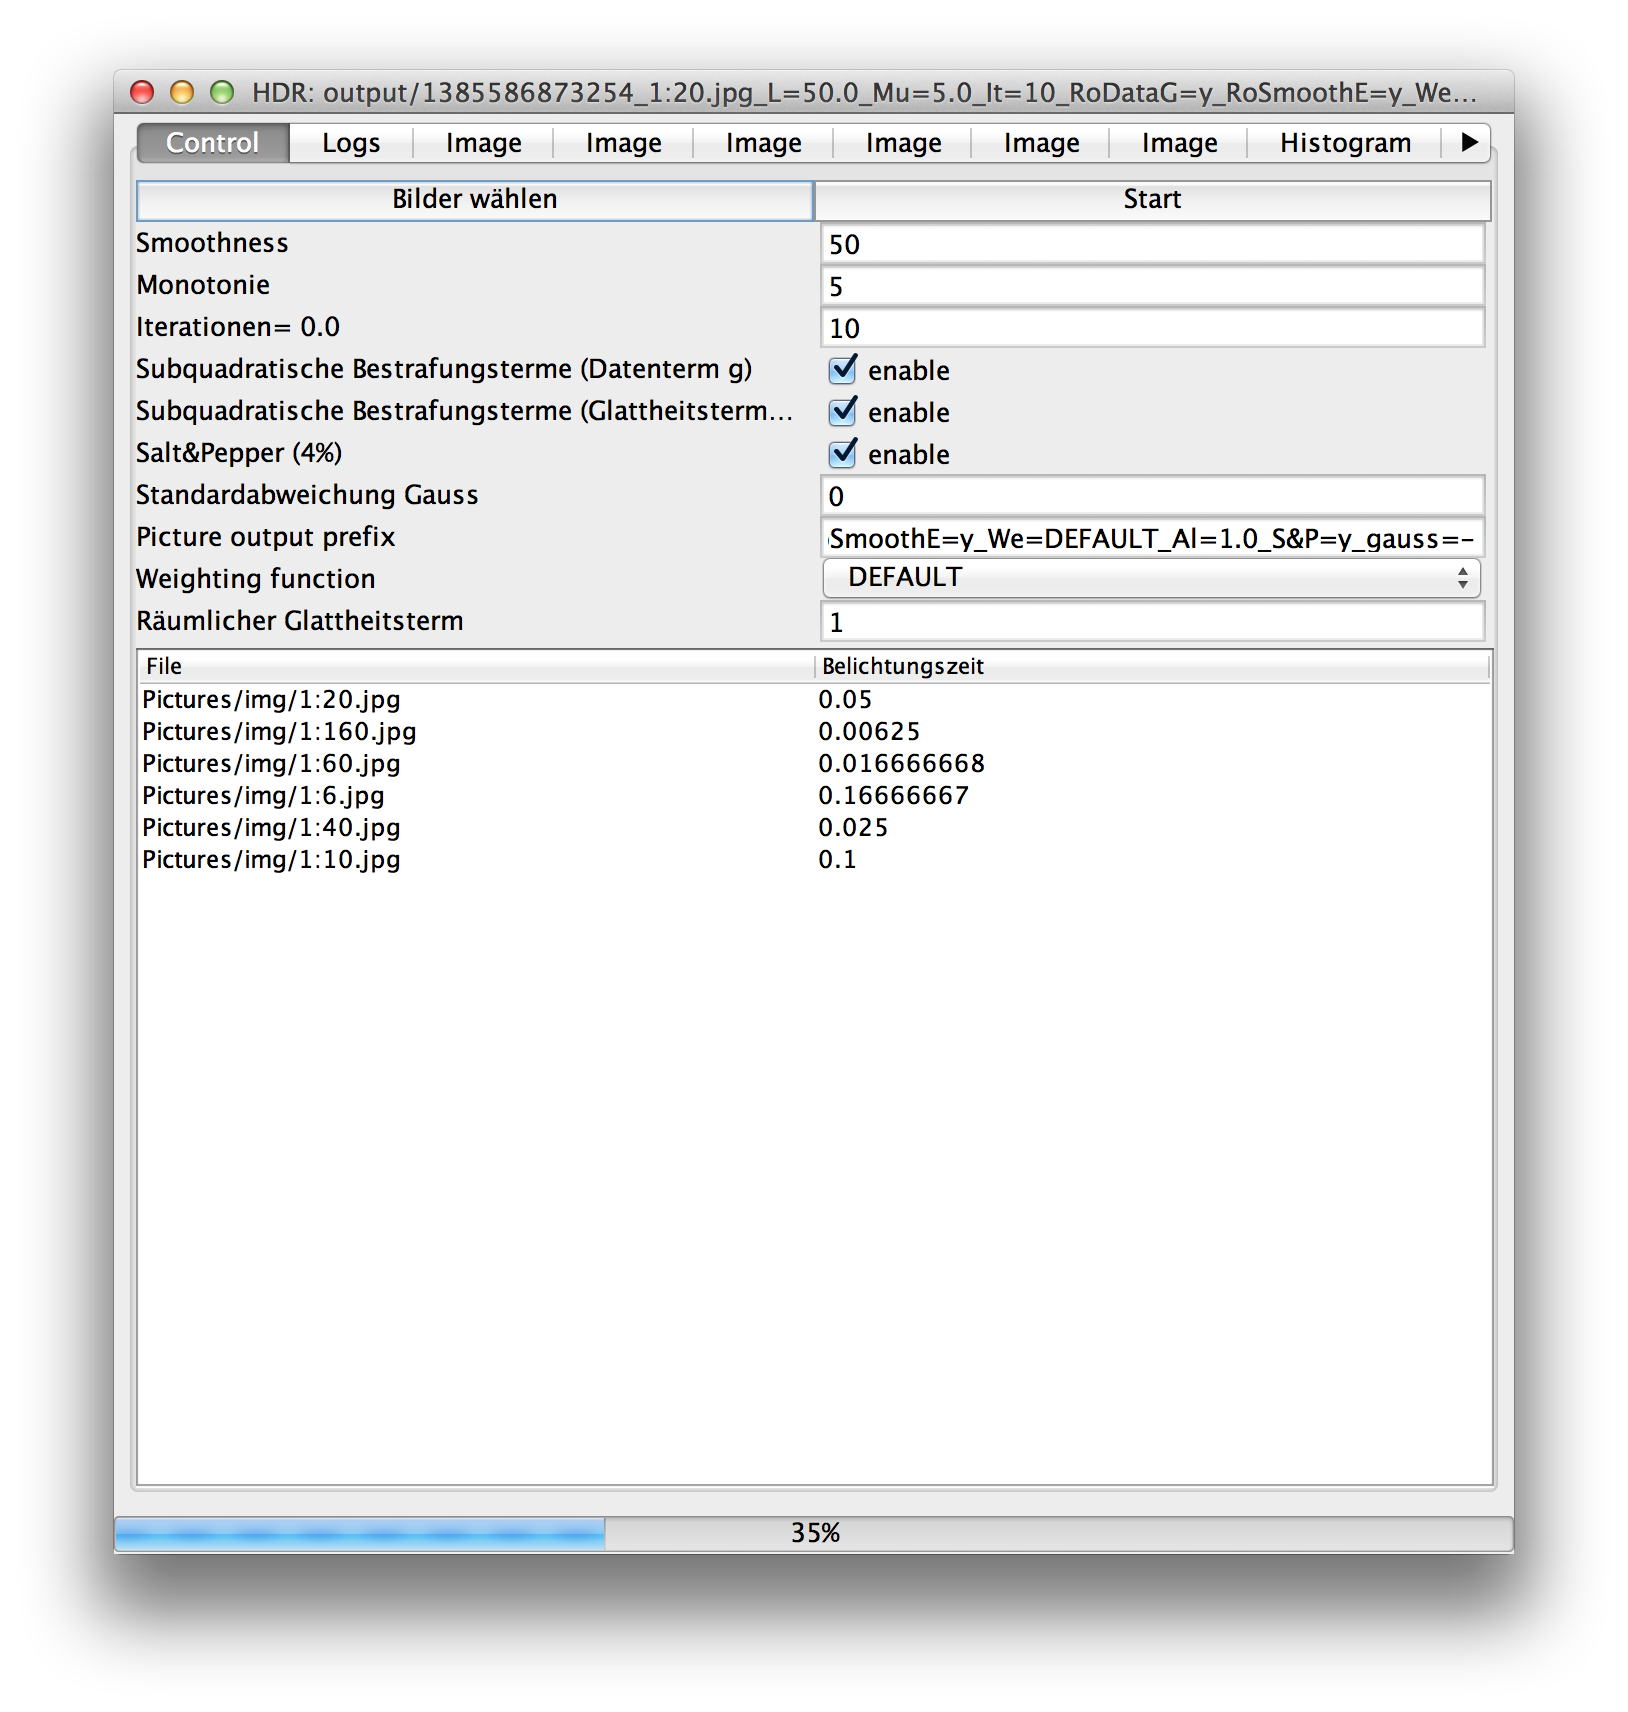
\includegraphics[width=\textwidth]{Tool}
    \caption{Die absichtlich schlicht und pragmatisch gehaltene Benutzereingabe für die Erzeugung der HDR-Bilder.}
    \label{fig:tool}
  \end{center}
\end{figure}


\section{Externe Bibliotheken}
Für die Implementierung wurden einige bereits bestehenden Komponenten eingesetzt. Diese werden hier kurz beschrieben.

\subsubsection*{\texttt{NumericTextField}\footnote{\url{http://www.java2s.com/Code/Java/Swing-JFC/NumericTextField.htm}}}
Für die Eingabe der einzelnen Parameter wird eine Implementierung eines numerischen Textfeldes verwendet. Dieses verhindert ungültige Eingaben und erleichtert das Auslesen der numerischen Parameter.

\subsubsection*{\texttt{metadata-extractor}\footnote{\url{https://code.google.com/p/metadata-extractor/}}}
Die Bibliothek \texttt{metadata-extractor} wird verwendet um automatisiert aus Bilddateien die Belichtungszeit der Bilder auszulesen. Mit ihm wird auch das von Adobe entwickelte \texttt{xmp-core}\footnote{\url{http://www.adobe.com/devnet/xmp.html}} mit geliefert. Zusammen genommen ermöglicht die Bibliothek die Belichtungszeiten der Bilder auszulesen und darzustellen.

\subsubsection*{\texttt{JImageChooser} \footnote{\url{http://docs.oracle.com/javase/tutorial/uiswing/examples/components/index.html\#FileChooserDemo2}}} 
Der verwendete \texttt{JFileChooser} zur Selektion von Bilddateien (und nur diesen) ist inspiriert von dem vorhandenen Tutorial bei Oracle. Er ist in der Lage eine kleine Vorschau der Bilder anzuzeigen.


\section{Architektur}
\label{sec:architektur}
Bei der Architektur der Software wurde eine \gls{MVC} Struktur eingehalten. Dieses Pattern beschreibt eine klare Trennung zwischen Datendarstellung, -verarbeitung und -repräsentation. Diese Teilung in drei Schichten sorgt dafür, dass die einzelnen Komponenten gut getestet werden können und beliebig austauschbar sind. Dadurch besteht ein hoher Grad an Erweiterbarkeit, da die Kopplung zwischen den Modulen möglichst gering gehalten wird.



\subsection{Komponentendiagramm}
Die Anwendung lässt sich grundsätzlich in fünf verschiedene Komponenten trennen (siehe \autoref{fig:arch:components}). 
\begin{description}
\item{\texttt{View}:} Das Paket \texttt{View} behandelt die gesamte Darstellung der Anwendung und die grafische Auswertung der berechneten Bilder. Es enthält \gls{Tone-Mapping} Operatoren und behandelt die Benutzereingabe.
\item{\texttt{Model}:} Das \texttt{Model} besteht in erster Linie aus den Beiden Klassen \texttt{Image} und \texttt{HDRResult}. Erstere wird als Repräsentation eines Bildes verwendet und speichert Grauwerte, Belichtungszeiten und weitere Bildrelevante Informationen. Letztere dient als Kommunikationspaket zwischen dem eigentlichen \texttt{Solver} und der restlichen Anwendung und enthält die fertig berechnete Antwortkurve und die \gls{Radiance Map}.
\item{\texttt{Ctrl}:} Dieses Paket dient zur Steuerung der Anwendung. In diesem werden die Eingaben verarbeitet, an die Algorithmen weiter gegeben und anschließend wieder dargestellt.
\item{\texttt{Maths}:} Die \texttt{Maths}-Komponente enthält alle notwendigen mathematischen Berechnungen und Repräsentationen, wie z.B. \texttt{Matrix} und \texttt{Vector}.
\end{description}

\begin{figure}[H]
  \begin{center}
    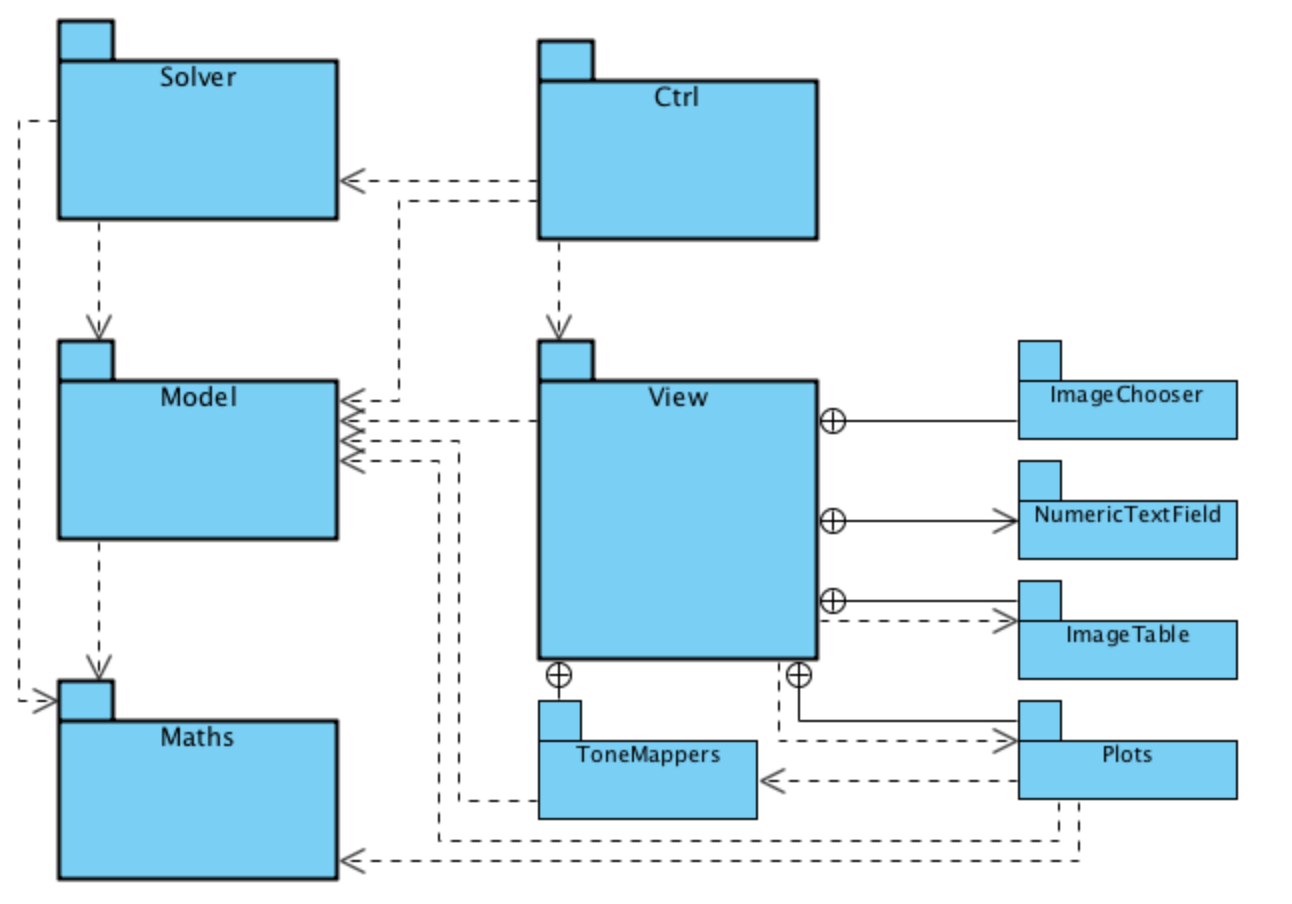
\includegraphics[width=0.8\textwidth]{architecture/components}
    \caption{Die Architektur der Software auf Komponentenebene. Hier kann gut die Trennung zwischen den einzelnen Bereichen erkannt werden.}
    \label{fig:arch:components}
  \end{center}
\end{figure}


\begin{figure}[H]
  \begin{center}
    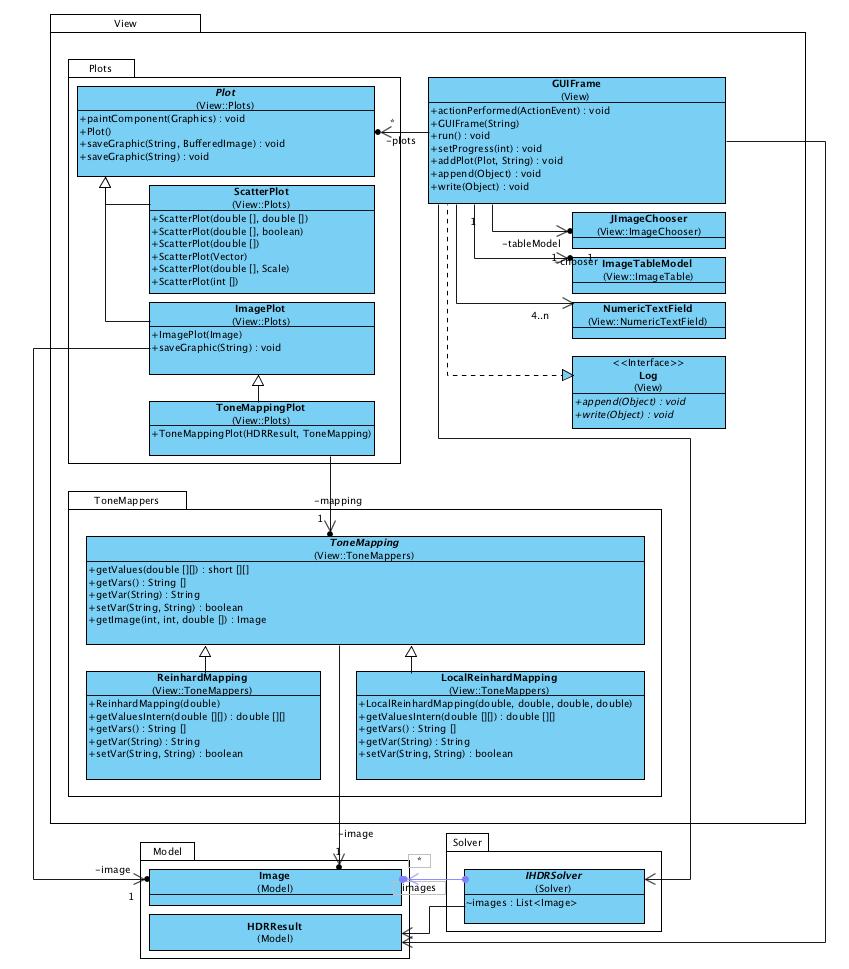
\includegraphics[width=0.8\textwidth]{architecture/view}
    \caption{Die \texttt{View}-Komponente im Detail. Das Hauptfenster \texttt{GUIFrame} stellt die Daten dar und importiert dazu die verschiedenen Komponenten. Die \texttt{Plots} und die \texttt{ToneMappers} gehören ebenfalls zu diesem Paket.}
    \label{fig:arch:plots}
  \end{center}
\end{figure}


\begin{figure}[H]
  \begin{center}
    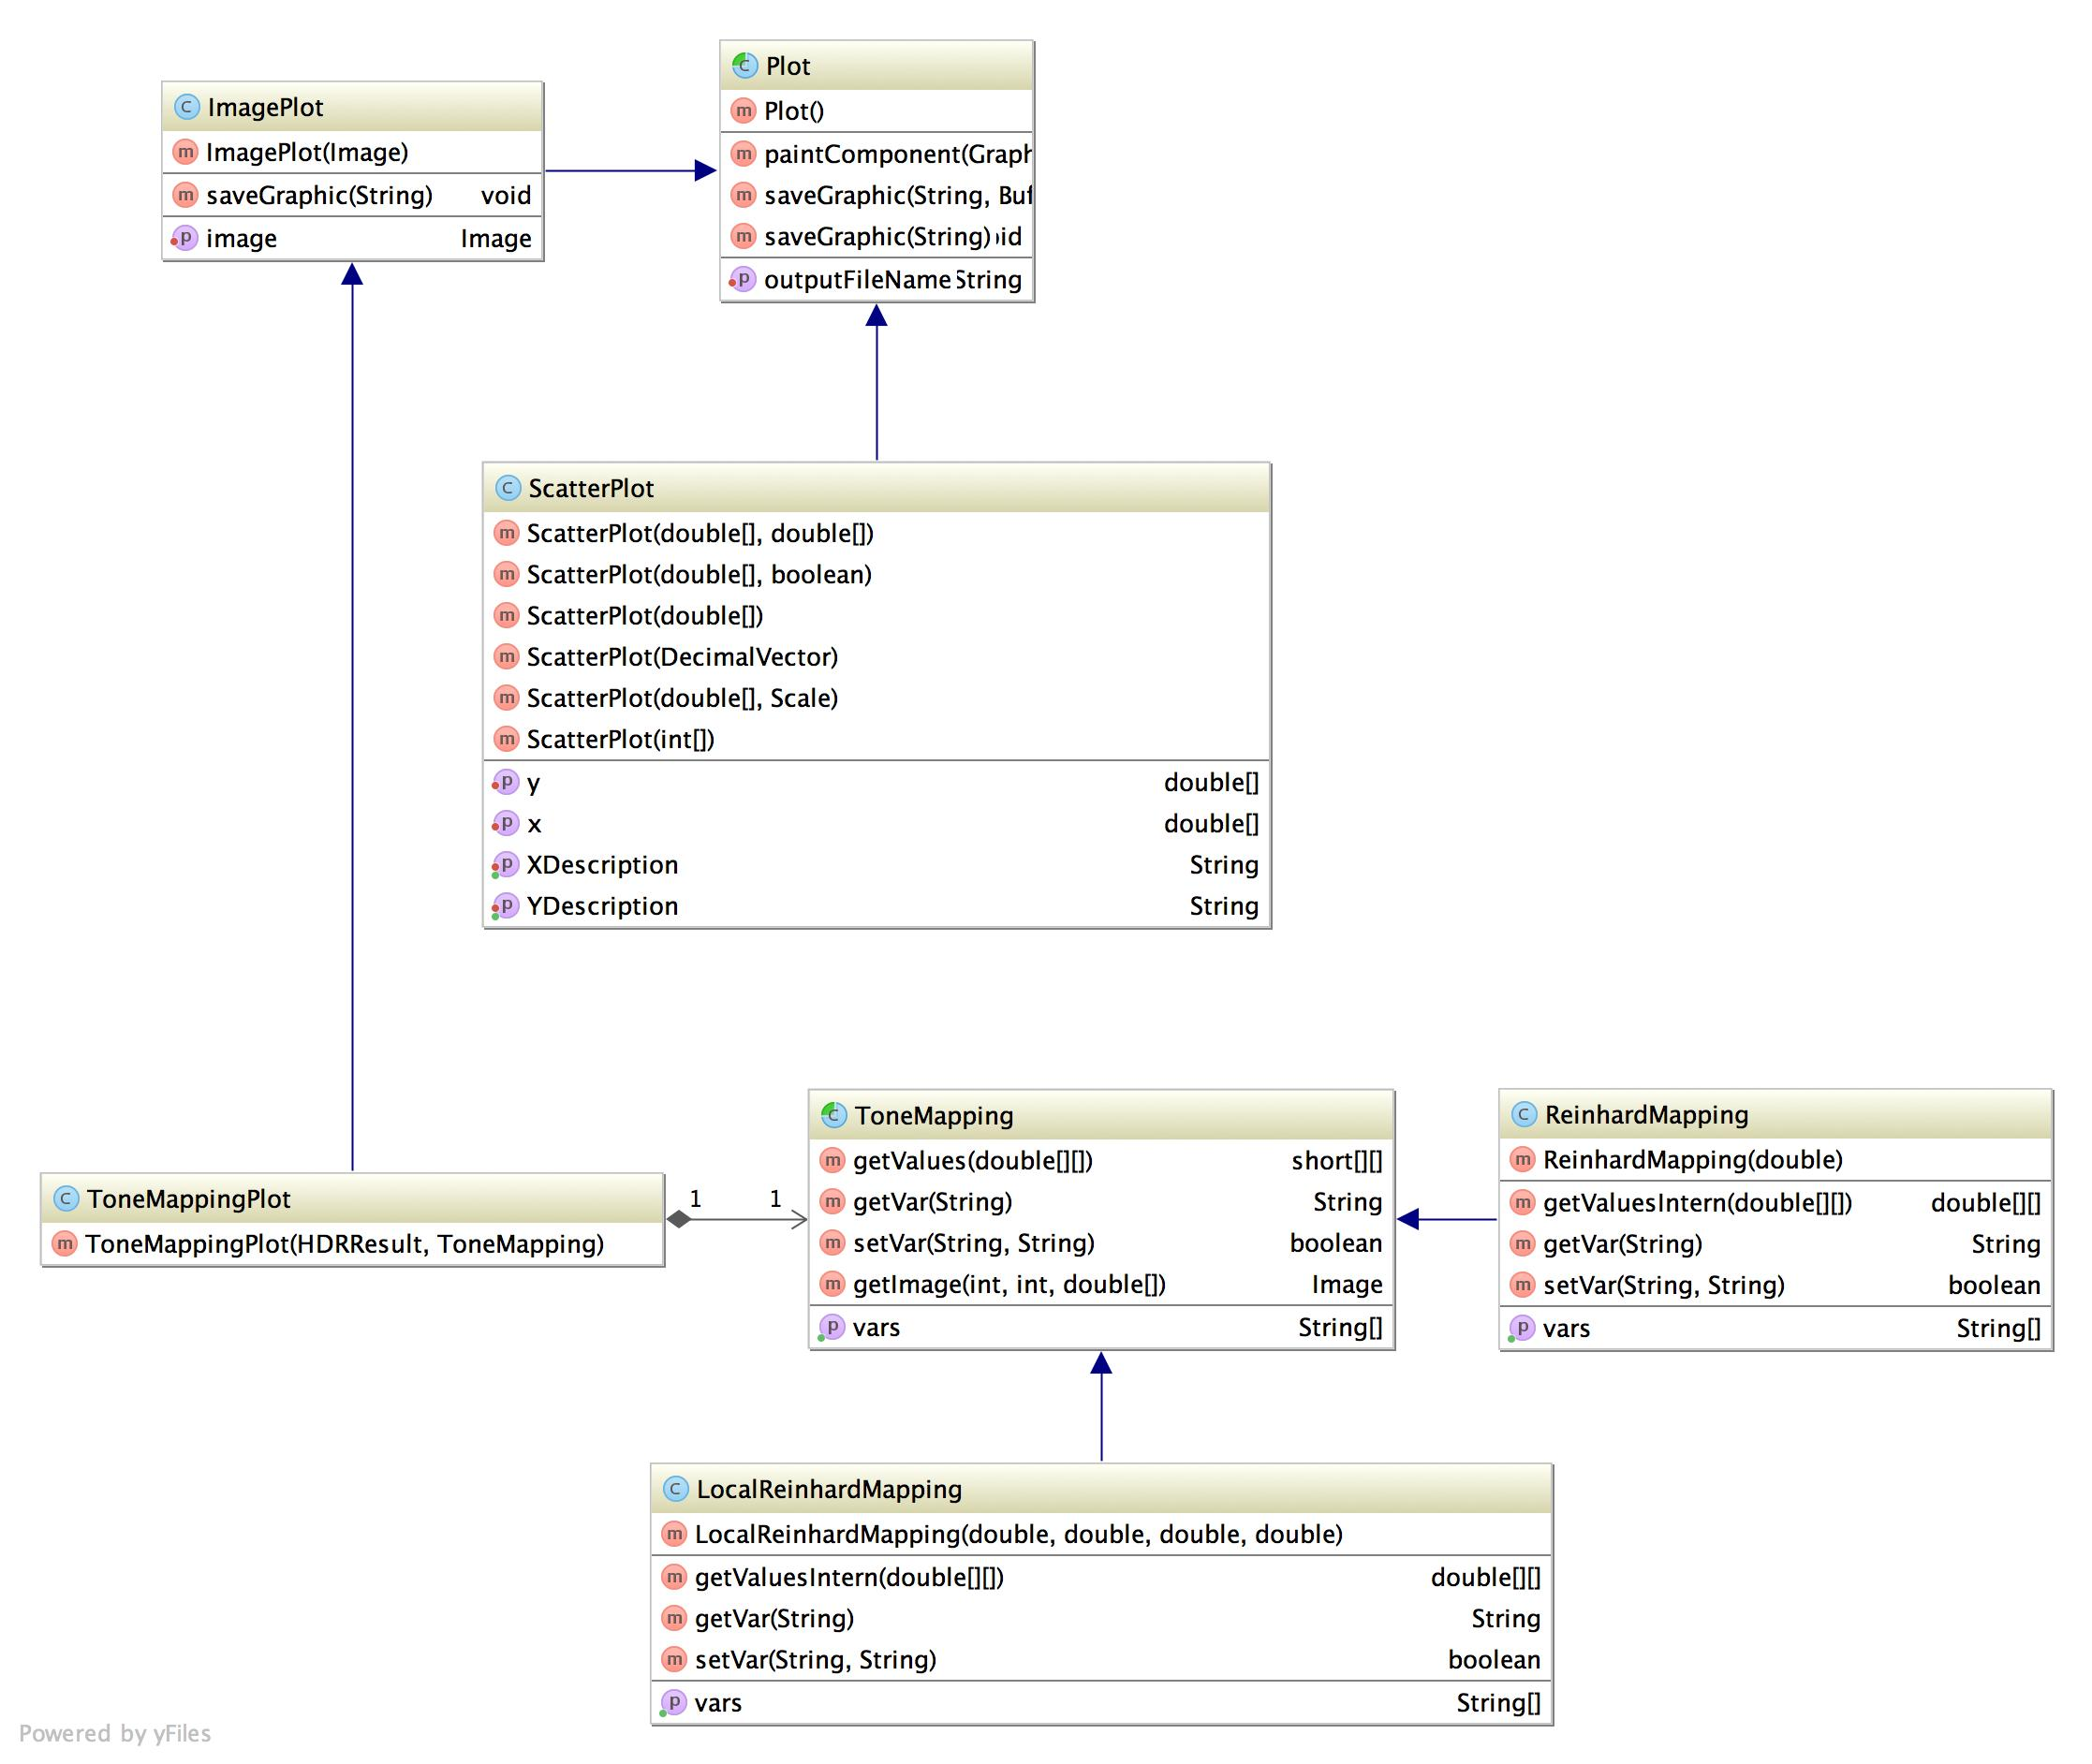
\includegraphics[width=0.8\textwidth]{architecture/plots}
    \caption{Die Struktur der verschiedenen grafischen Plots. Die Implementierungen von verschiedenen \gls{Tone-Mapping} Operatoren mittels Vererbung kann hier gut erkannt werden.}
    \label{fig:arch:plots}
  \end{center}
\end{figure}


\begin{figure}[H]
  \begin{center}
    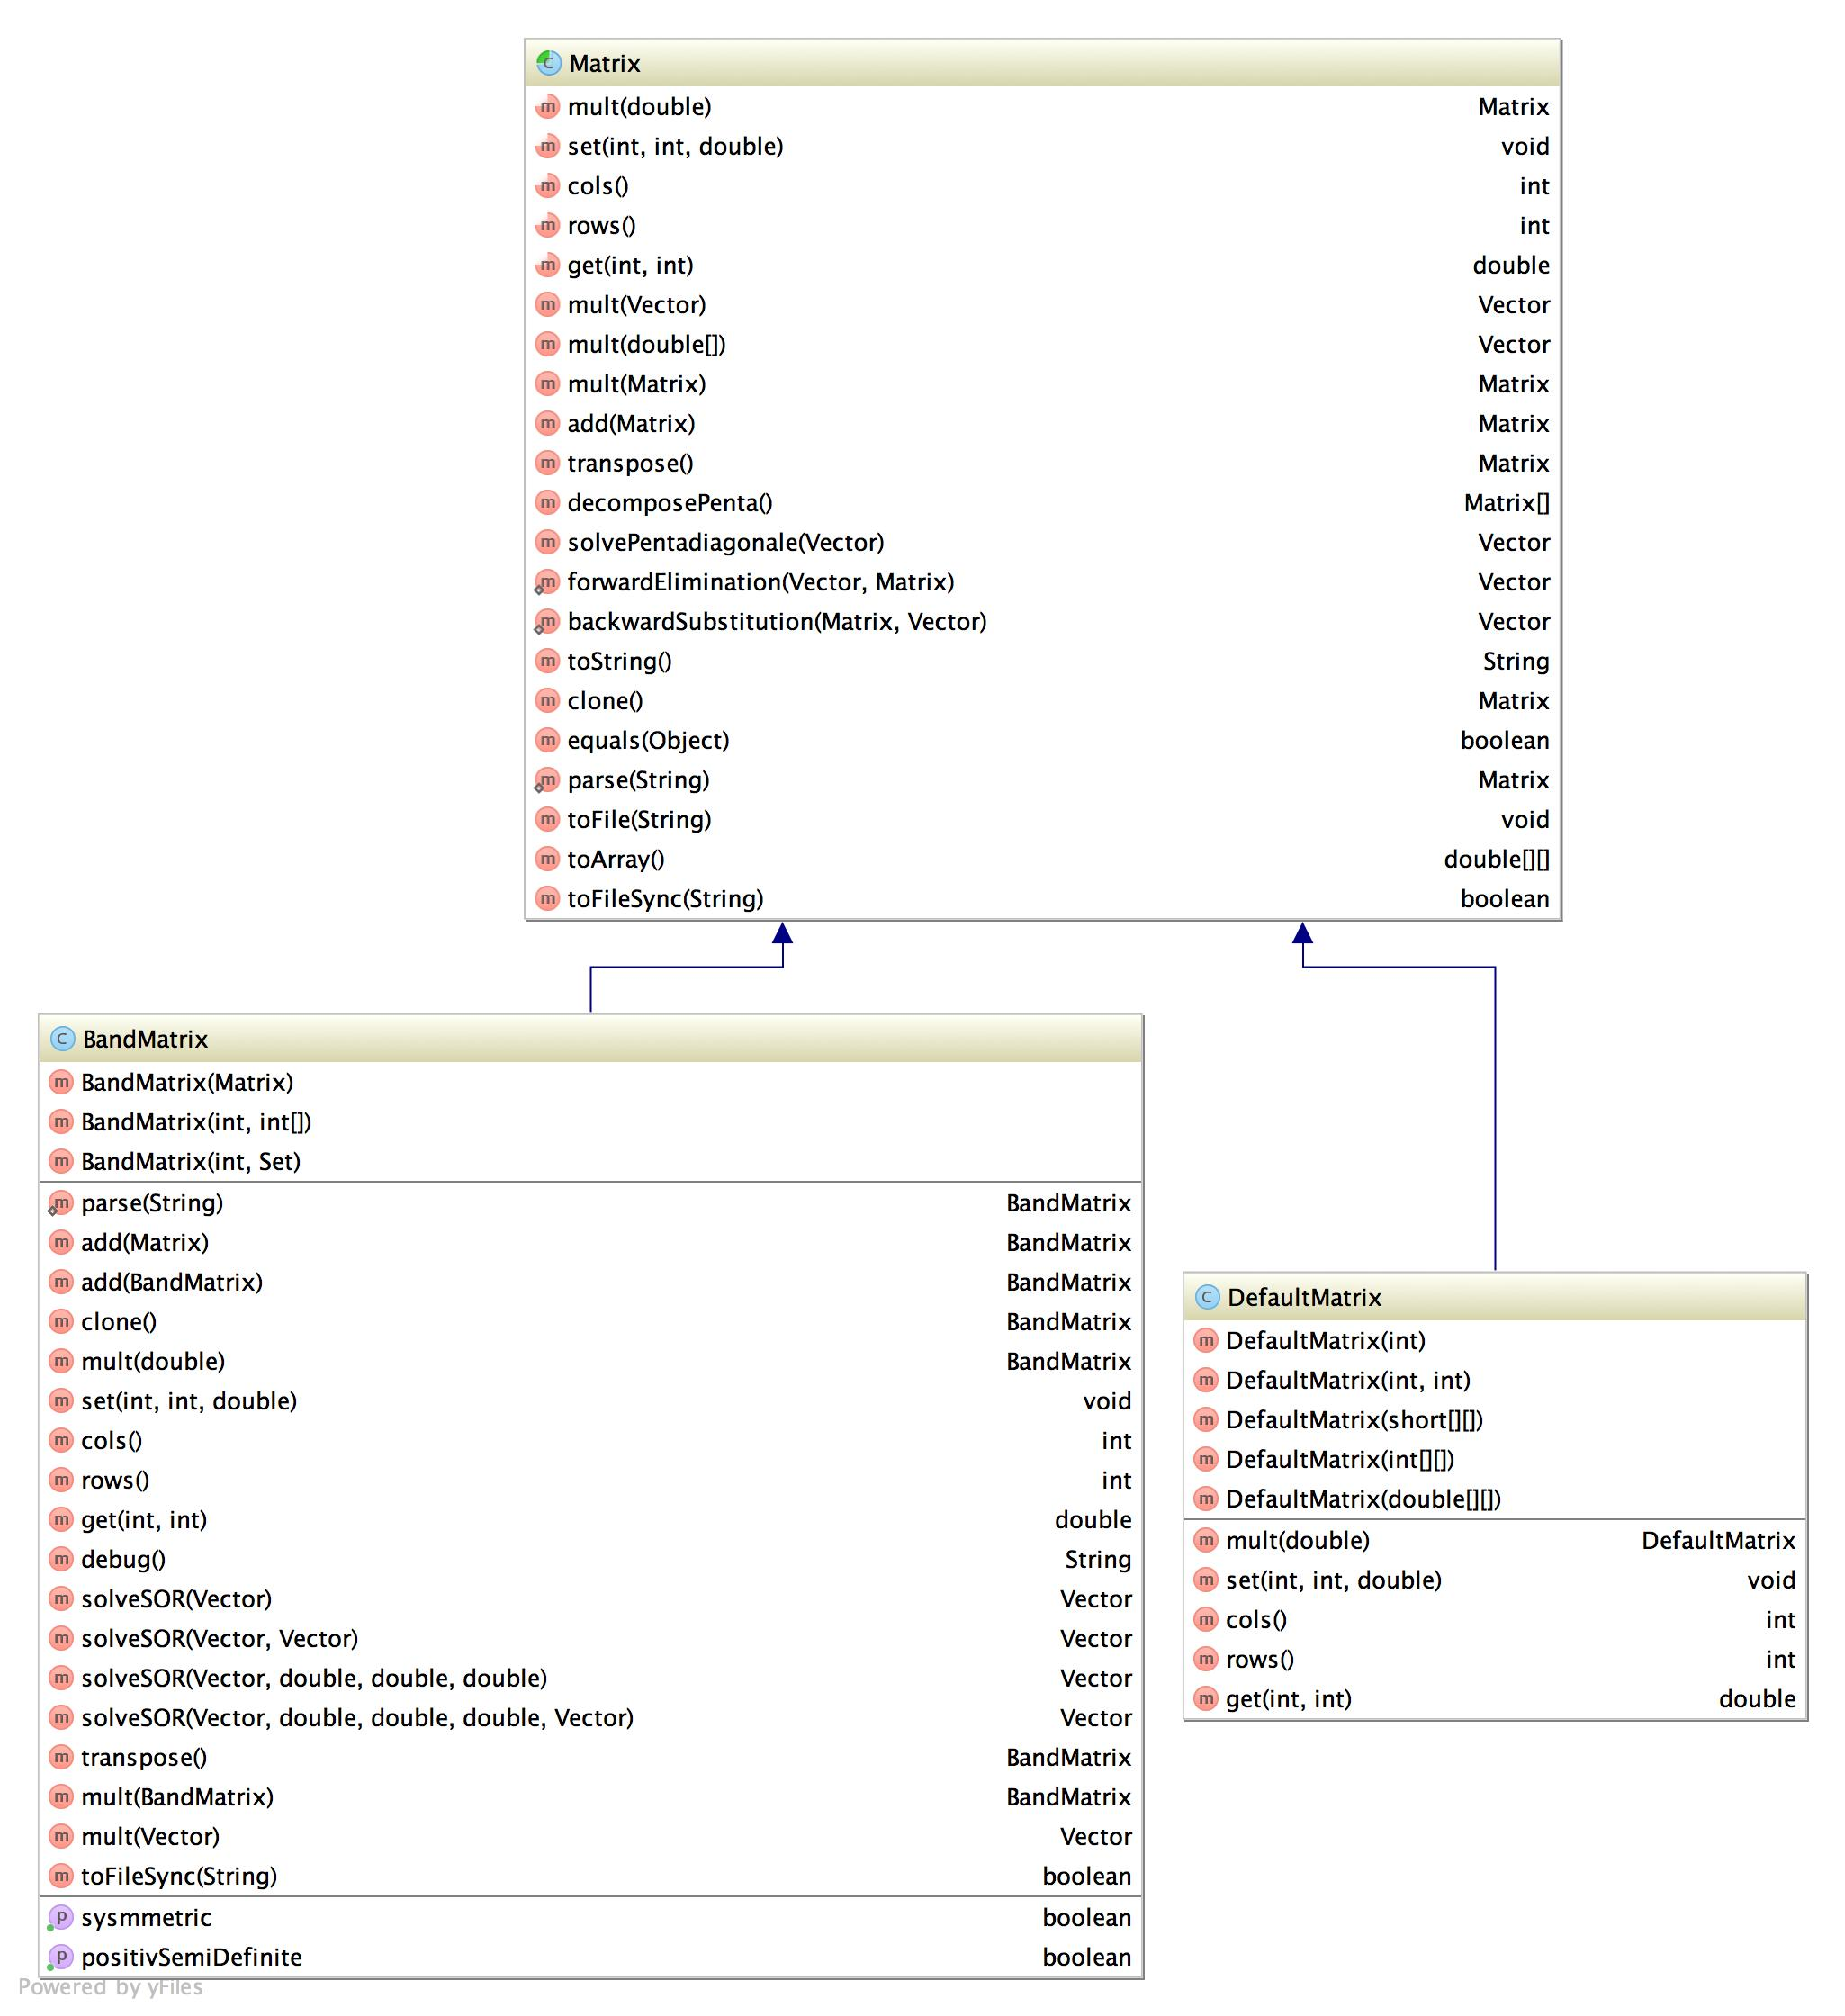
\includegraphics[width=\textwidth]{architecture/matrixes}
    \caption{Die Klasse \texttt{Matrix} und ihre Spezialisierungen \texttt{BandMatrix} und \texttt{DefaultMatrix}. Diese beiden Klassen dienen zusammen mit \texttt{Vector} als ein Kernbestandteil der mathematischen Berechnungen dieses Programmes.}
    \label{fig:arch:plots}
  \end{center}
\end{figure}


\subsection{Sequenzdiagramm}
Das Programm läuft sehr vielschichtig ab. Als grundsätzliche Architekturüberlegung stand jedoch zu Beginn der Aufbau wie in \autoref{fig:arch:sequence} beschrieben ist. Wichtig dabei ist, dass die grafische Benutzeroberfläche nicht von der Berechnungsdauer des Algorithmus blockiert wird, weshalb besonders zwischen \texttt{Controller} und \texttt{GUIFrame} asynchrone Methodenaufrufe zum Einsatz kommen.
\begin{figure}[H]
  \begin{center}
    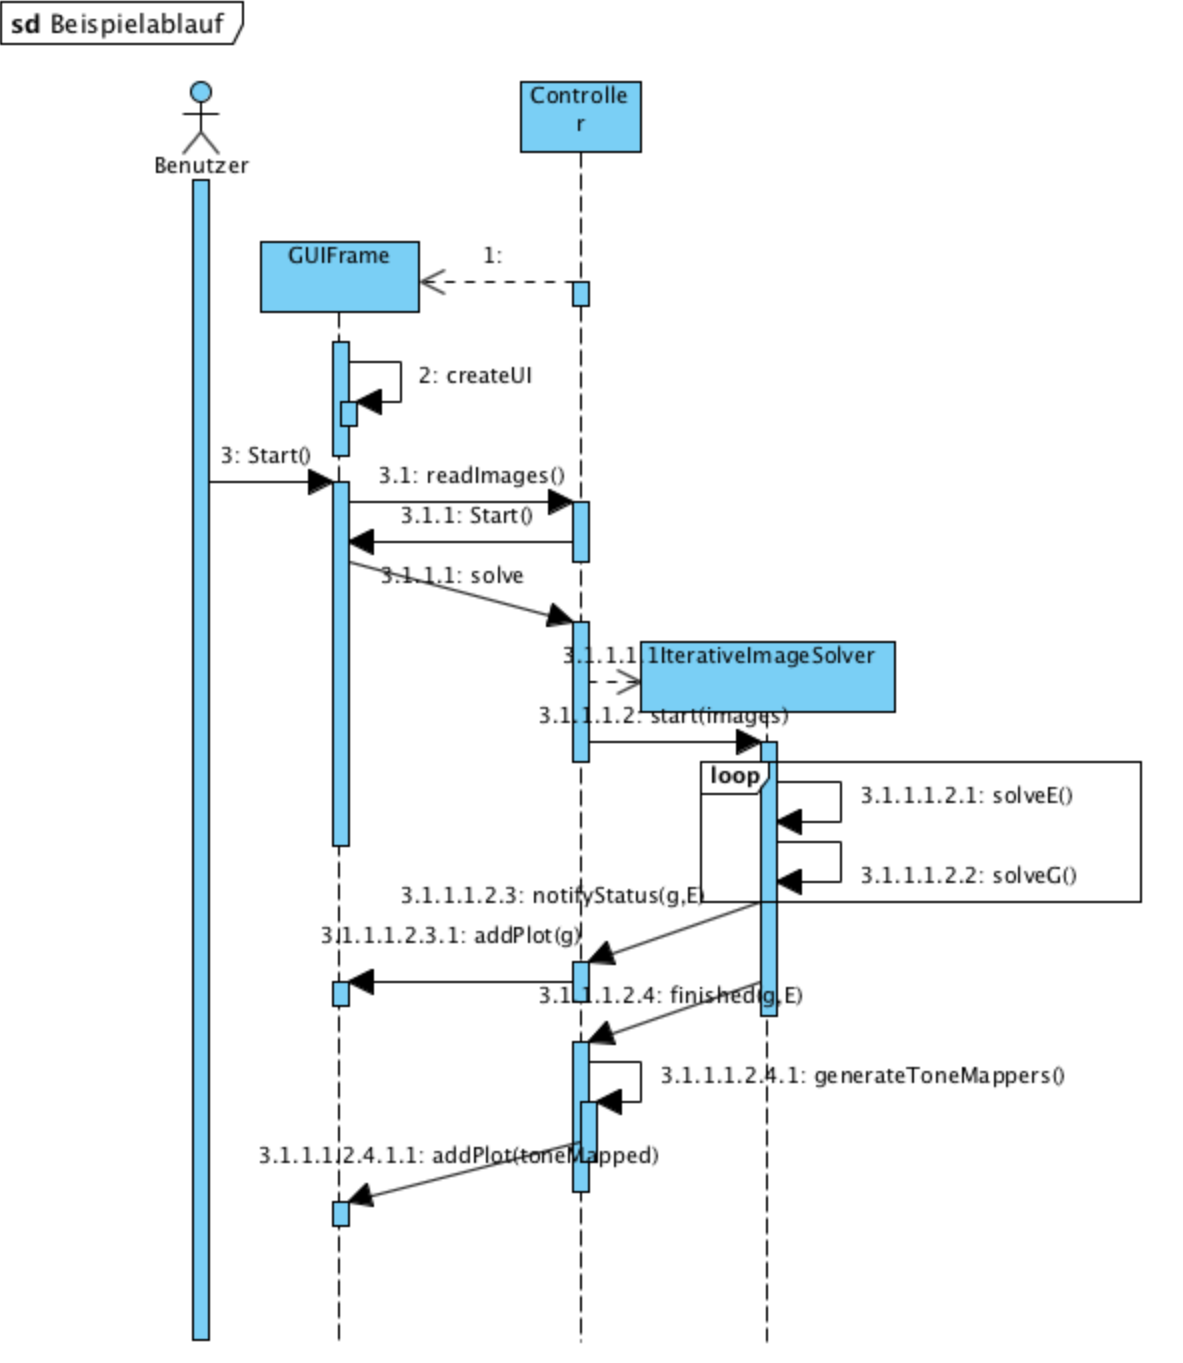
\includegraphics[width=0.8\textwidth]{architecture/sequence_example}
    \caption{Der grundsätzliche Ablauf der Berechnung des HDR-Bildes und der Antwortkurve und der dabei beteiligten Komponenten sowie deren Interaktion. }
    \label{fig:arch:sequence}
  \end{center}
\end{figure}

\section{Algorithmus in Pseudocode}
\label{sec:pseudocode}
\section{Ausgewählte Programmabschnitte}
\label{sec:sample-codes}
\section{Verwendetes \gls{Tone-Mapping}-Verfahren}
\label{sec:tone-mapping}
\section{Laufzeitanalyse}
\label{sec:laufzeit}



%Die Angabe des schlauen Spruchs auf diesem Wege funtioniert nur,
%wenn keine Änderung des Kapitels mittels den in preambel/chapterheads.tex
%vorgeschlagenen Möglichkeiten durchgeführt wurde.
\setchapterpreamble[u]{%
\dictum[Albert Einstein]{Probleme kann man niemals mit derselben Denkweise lösen, durch die sie entstanden sind.}
}
\chapter{Ergebnisse und Resultate}
\label{chap:results}

\section{Ergebnisse ohne Erweiterungen}

\section{Ergebnisse mit Erweiterungen}

\subsection{Ergebnisse mit \glspl{Robustheit}-Term}
\subsection{Ergebnisse mit \gls{Monotonie}-Bedingung}
\subsection{Ergebnisse mit räumlichem Glattheitsterm}

\section{Vergleich der Ergebnisse}

\section{Vergleich zum naiven Ansatz von Debevec und Malik \cite{paper}}


\chapter{Zusammenfassung und Ausblick}
\label{chap:zusfas}
\texttt{T.B.D}

\section*{Ausblick}
\texttt{T.B.D}



%
%
%\renewcommand{\appendixtocname}{Anhang}
%\renewcommand{\appendixname}{Anhang}
%\renewcommand{\appendixpagename}{Anhang}
\appendix
\chapter{Anhang}
\section{Artikel \cite{paper}}
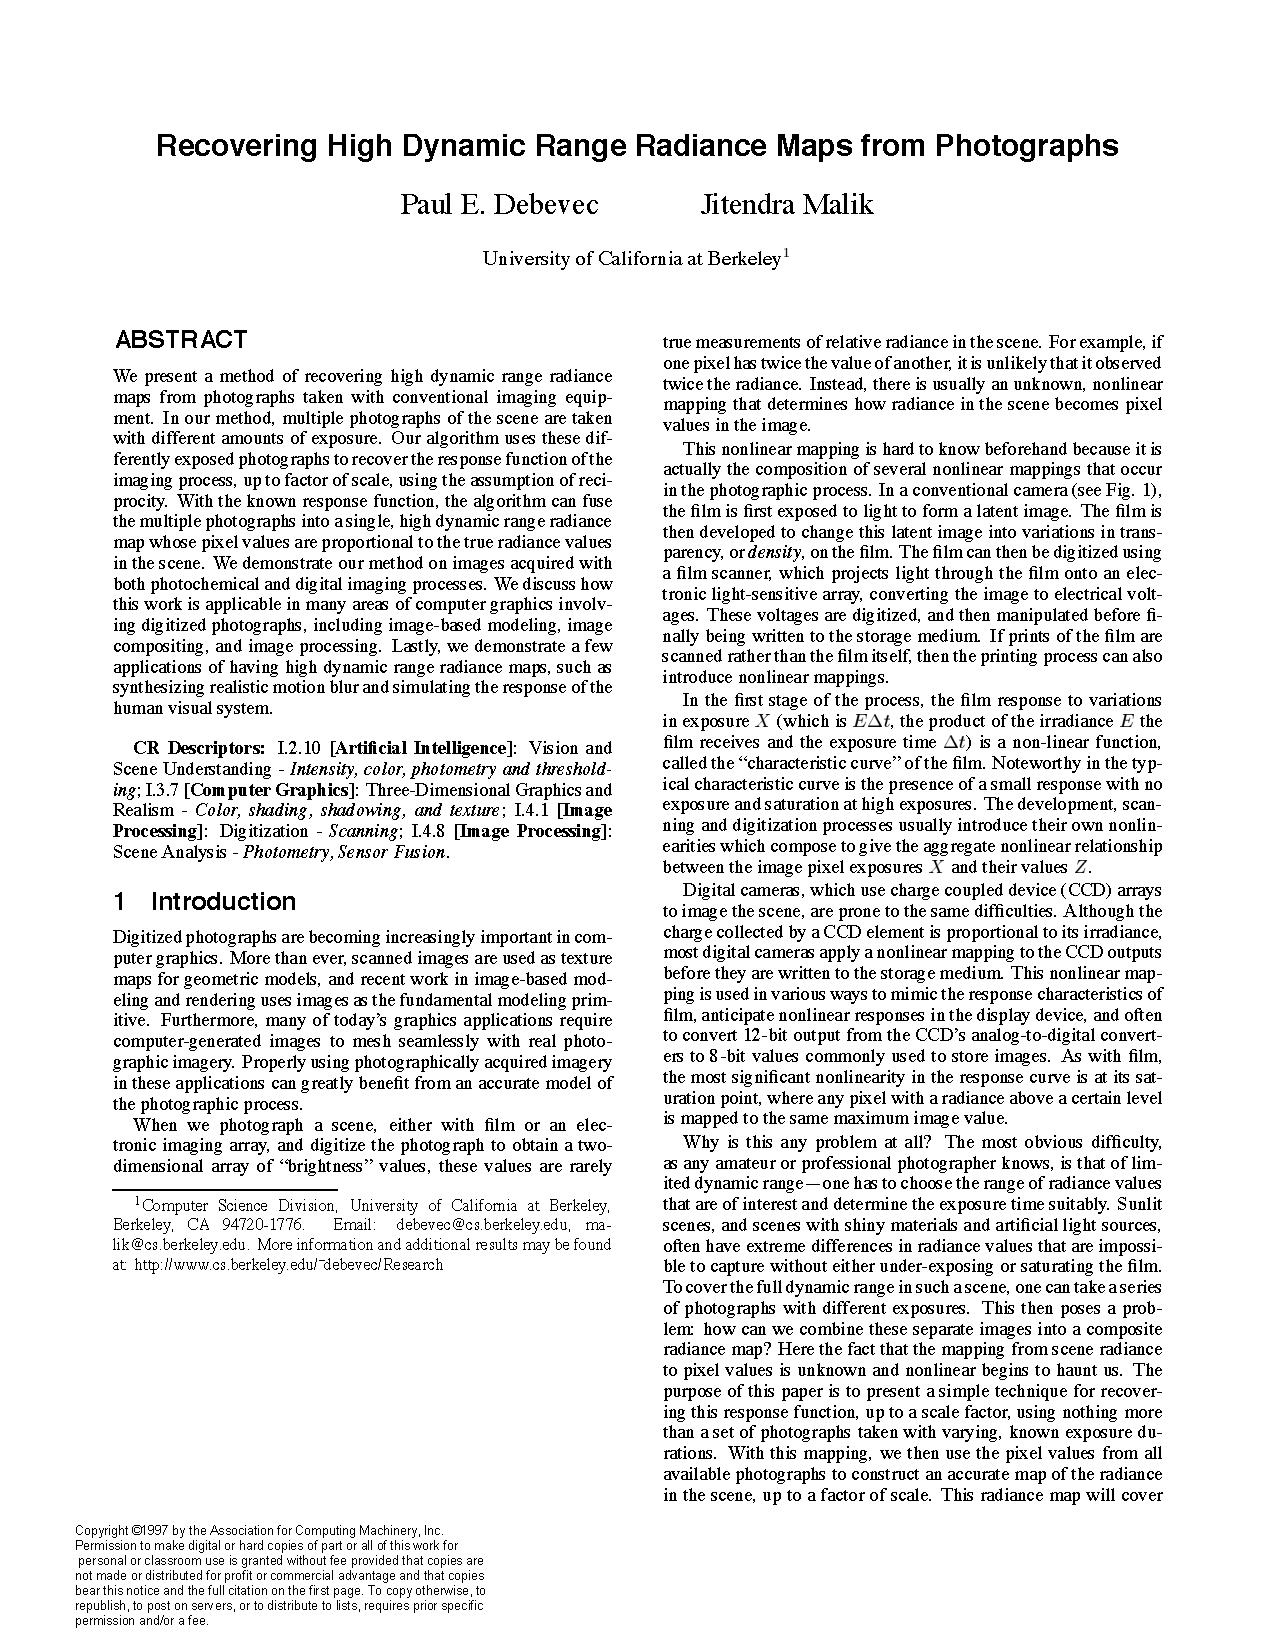
\includepdf[pagecommand={},pages=-,scale=0.8]{content/attachment/00_Artikel.pdf} 
\section{Verwendete Algorithmen}

\subsection{MTB-Algorithmus, vgl. \cite[S.9 f]{Ward03fast}}
\label{subsec:MTB}
Dem \gls{MTB} Verfahren (vgl. \cite{Ward03fast}) wird eine Serie von $N$ Bildern als Eingabe geliefert. Diese werden zunächst in ein Grauwert-Bild umgerechnet. Aus diesen Bildern wird der Algorithmus dann ausgehend von einem gewähltem Bild $N-1$ Offsets $(x,y)$ ausgeben, sodass die Bilder exakt übereinander gelegt werden können (vgl. \cite[S. 123f]{Reinhard}). Eine Alignierung von rotierten Bildern ist somit mit diesem Verfahren nicht möglich. 

Das Verfahren arbeitet dabei im Gegensatz zu vielen konventionellen Algorithmen nicht mit Kanten-Detektion im Bild um die Alignierung durchzuführen, da diese sehr anfällig auf unterschiedliche Belichtungswerte in Bildern sind. Es kommt hingegen ein Schwellwert-Verfahren auf einer Bilderpyramide zum Einsatz, dass dann mit schnellen Bit-Operationen die Verschiebung der Bilder berechnet (vgl. \cite{Ward03fast}). Der Code dazu befindet sich im Anhang (siehe \autoref{lst:MTB:core}).

\begin{Listing}[H]
\label{lst:MTB:helpers}
\begin{lstlisting}[language=c]
/** Subsample the image img by a factor of two in each dimension 
 *  and put the result into a newly allocated image img_ret.*/
ImageShrink2(const Image *img, Image *img_ret)

/** Allocate and compute the threshold bitmap tb and the exclusion bitmap eb for the image img. 
 *  (The threshold and tolerance to use are included in the Image struct.)*/
ComputeBitmaps(const Image *img, Bitmap *tb, Bitmap *eb)

/** Shift a bitmap by (xo,yo) and put the result into the preallocated 
 *  bitmap bm_ret, clearing exposed border areas to zero. */
BitmapShift(const Bitmap *bm, int xo, int yo, Bitmap *bm_ret)

/** Compute the exclusive-or of bm1 and bm2 and put the result into bm_ret. */
BitmapXOR(const Bitmap *bm1, const Bitmap *bm2, Bitmap *bm_ret)

/** Compute the sum of all 1 bits in the bitmap. */
BitmapTotal(const Bitmap *bm)
\end{lstlisting}
\caption{Hilfsfunktionen in C Funktion zur Berechnung der Alignierung}

\end{Listing}

\begin{Listing}[H]
\label{lst:MTB:core}
\begin{lstlisting}[language=c]
/** Computes the shift between two images img1 and img2.**/
GetExpShift(const Image *img1, const Image *img2, int shift_bits, int shift_ret[2])
{
    int min_err;
    int cur_shift[2]; Bitmap tb1, tb2; Bitmap eb1, eb2;
    int i, j;
    if (shift_bits > 0) {
        Image sml_img1, sml_img2;
        ImageShrink2(img1, &sml_img1);
        ImageShrink2(img2, &sml_img2);
        GetExpShift(&sml_img1, &sml_img2, shift_bits-1, cur_shift); ImageFree(&sml_img1);
        ImageFree(&sml_img2);
        cur_shift[0] *= 2;
        cur_shift[1] *= 2;
    } else
    cur_shift[0] = cur_shift[1] = 0;
    ComputeBitmaps(img1, &tb1, &eb1);
    ComputeBitmaps(img2, &tb2, &eb2);
    min_err = img1->xres * img1->yres;
    for (i = -1; i < = 1; i++)
    for (j = -1; j <= 1; j++) {
        int xs = cur_shift[0] + i;
        int ys = cur_shift[1] + j;
        Bitmap shifted_tb2;
        Bitmap shifted_eb2;
        Bitmap diff_b;
        int err;
        BitmapNew(img1->xres, img1->yres, &shifted_tb2); BitmapNew(img1->xres, img1->yres, &shifted_eb2); BitmapNew(img1->xres, img1->yres, &diff_b); BitmapShift(&tb2, xs, ys, &shifted_tb2); BitmapShift(&eb2, xs, ys, &shifted_eb2); BitmapXOR(&tb1, &shifted_tb2, &diff_b); BitmapAND(&diff_b, &eb1, &diff_b); BitmapAND(&diff_b, &shifted_eb2, &diff_b);
        err = BitmapTotal(&diff_b);
        if (err < min_err) {
            shift_ret[0] = xs;
            shift_ret[1] = ys;
            min_err = err;
        }
        BitmapFree(&shifted_tb2);
        BitmapFree(&shifted_eb2);
    }
    BitmapFree(&tb1); BitmapFree(&eb1);
    BitmapFree(&tb2); BitmapFree(&eb2);
}
\end{lstlisting}
\caption{Rekursive C Funktion zur Berechnung der notwendigen Verschiebung zwischen den Bildern um diese zu alignieren}
\end{Listing}

\subsection{LU-Zerlegung}
\begin{Algorithmus}[H]
\caption{Lösen von $A\cdot x = b$ mittels LU-Zerlegung (A ist pentadiagonal)}
\label{alg:LU}
\begin{algorithmic}
\Function{LUDecomposition}{$A$}
	\If{!\Call{isPentadiagonale}{$A$}}
	    \State \Return error
	\EndIf
    \State $m_0 \gets A_{0,0}$, $\qquad r_0 \gets A_{0,1}$, $\qquad l_0 \gets A_{1,0}/m_0$, $ \qquad m_1 \gets A_{1,1}- l_1r_0$
    \ForAll{$i \in [2,n]$}
        \State $p_i \gets A_{i-2,i}$
        \State $k_i \gets A_{i,i-2}/m_{i-2}$
        \State $r_{i-1} \gets A_{i-1,i} - l_{i-1}  p_{i-2}$
        \State $m_i \gets A_{i,i} - k_i p_{i-2} - l_i  r_{i-1}$
        \State $l_i \gets (A_{i,i-1}-k_i r_{i-2})/m_{i-1}$
    \EndFor
    \State $L \gets $\Call{generateL}{$l$, $k$}         \Comment{Generiert die Matrix L und U }
    \State $U \gets $\Call{generateU}{$m$, $r$, $p$}    \Comment{nach obigem Schema (siehe \autoref{eq:lu:structure})}
    \State \Return [L, U]
\EndFunction

\Function{forwardElimination}{b,L}
        \State $y_0 \gets b_0$
        \State $y_1 \gets b_1 - L_{1,0} y_0$
        \For{$i = 2 \mbox{ to } size(b)$}
            \State $y_i \gets b_i - L_{i,i-2} y_{i-2} - L_{i,i-1} y_{i-1}$
        \EndFor
        \Return $y$
\EndFunction


\Function{backwardSubstitution}{U,y}
        \State $x_{n-1} \gets y_{n-1}/U_{n-1,n-2}$
        \State $x_{n-2} \gets (y_{n-2} - U_{n-2,n-1} x_{n-1})/U_{n-2,n-2}$
        \State $y_1 \gets b_1 - L_{1,0} y_0$
        \For{$i = size(b)-3 \mbox{ to } 0$}
            \State $x_i \gets (U_{i,i+1} x_{i+1}- U_{i,i+2} x_{i+2} - y_i) / U_{i,i}$
        \EndFor
        \Return $x$
\EndFunction




\Function{Solve}{$A$, $b$}
	\If{\Call{size}{$A$} != \Call{size}{b}}
	    \State \Return error
	\EndIf
	\State [L,U] = \Call{LUDecomposition}{A};

    \State $y \gets $\Call{forwardElimination}{b, L} \Comment{forward elimination L*y = b}
    \State $x \gets $\Call{backwardSubstitution}{U,y} \Comment{backward substitution U*x = y}
    \State \Return $x$
\EndFunction
\end{algorithmic}
\end{Algorithmus}



\section{Programmcode}

%\printindex
%\bibliographystyle{alphadin}

\addcontentsline{toc}{chapter}{Glossar}
\glossarystyle{altlist}
\printglossary % if no option is supplied the default glossary is printed.


\ifdeutsch
\bibliographystyle{bibliography/IAASde} %f"ur deutsche Texte
\else
\bibliographystyle{bibliography/IAAS} %f"ur englische Texte
\fi
\bibliography{bibliography/bibliography}
Alle URLs wurden zuletzt am 27.\,11.\,2013 geprüft.
\backmatter 
\pagestyle{empty}
\renewcommand*{\chapterpagestyle}{empty}
\Versicherung
\end{document}
